%
% This program is free software: you can redistribute it and/or modify
% it under the terms of the GNU General Public License as published by
% the Free Software Foundation, either version 3 of the License, or
% (at your option) any later version.

% This program is distributed in the hope that it will be useful,
% but WITHOUT ANY WARRANTY; without even the implied warranty of
% MERCHANTABILITY or FITNESS FOR A PARTICULAR PURPOSE.  See the
% GNU General Public License for more details.

% You should have received a copy of the GNU General Public License
% along with this program.  If not, see <http://www.gnu.org/licenses/>.

\documentclass{book}

\usepackage{/home/gnustats/Documents/R-Project/ihelp/tutorial-dev/mystyle}

\title{R 스터디 가이드 \\
   - 도움이 되길 바랍니다 - 
   }
\author{iHELP Working Group \\ Chel Hee Lee \& Eugene Jung } 
\date{\today}

\begin{document}
\maketitle
\tableofcontents 

% %
% Author: Chel Hee Lee 
% Created on 2013-APR-10
% Modified on 2013-MAY-10
%

%  File tutorial-dev/Parts/part1-ch02.tex
%  Part of the iHELP project at http://ihelp.r-forge.r-project.org
%
%  Copyright (C) 2013- The iHELP Working Group 
%                                in the Korean R Translation Team
%
%  This program is free software; you can redistribute it and/or modify
%  it under the terms of the GNU General Public License as published by
%  the Free Software Foundation; either version 2 of the License, or
%  (at your option) any later version.
%
%  This program is distributed in the hope that it will be useful,
%  but WITHOUT ANY WARRANTY; without even the implied warranty of
%  MERCHANTABILITY or FITNESS FOR A PARTICULAR PURPOSE.  See the
%  GNU General Public License for more details.
%
%  A copy of the GNU General Public License is available at
%  http://www.r-project.org/Licenses/
%


% 정우준의 서두 -- 문서 보다는 개인적 블로그에 적합할 것 같아 넣지 않음. 
%
% 이런 느낌은 특히 최소한 내가 알기로는 경영학과 경제학 분야(거의 확실함) 및 사회학, 심리학 분야가 특히 심하다. 
% 그리고 이들 분야에서는 R의 다양한 기능(특히 visualization) 또는 packages를 필요로 하지 않을 가능성이 높다. 
% 왜냐하면 분석 방법이 단순하기 때문이다.
% 여기에서 분석 방법이 단순하다는 것은 그 이론적 배경이 쉽다는 것을 의미하는 것이 아니라 절차상의 얘기이다.
%
% 언급한 분야에서 학술연구에서 실행되는 분석의 양을 보면 대부분 [기술통계 - 상관관계 - 차이분석, 회귀분석, 구조방정식분석] 정도로 분석이 마무리 되기 때문이다. 
% 대부분 표(table)로 결과를 보고하는 형식을 따르고 있다.
% 분석 모형 자체를 다루는 연구가 거의 없는 것이다. 
% 따라서 R의 작업 방식은 그들에게는 불필요할 지도 모른다.

% 그러나 여전히 R의 다양한 source를 필요로 하는 아주 작은 규모의 학술연구 분야는 존재한다. 
% 따라서 여기의 tips에는 이들을 고려하여 R 사용에 도움이 될 만한 사항들을 정리하고자 한다.
% 개인적으로는 통계학 및 다른 분야의 연구 과정이 어떻게 진행되는지 잘 모르는 것도 한 몫하여 이에 해당하는 부분은 다른 이의 도움이 절실하다.

% 덧붙여 나는 윈도우 환경에서의 R tip에 주목하고자 한다(Mac이나 유닉스/리눅스 환경에서의 R 사용에 관한 tip도 다른 이의 도움이 필요한 부분이다). 
% 그 이유는 내가 윈도우에서 SPSS와 SAS를 숙련시켜 왔기 때문에 대부분의 통계분석 초심자들도 윈도우 환경에서 R 을 접하게 될 것이라는 막연한 억측 때문이다. 
% 시간이 지나면서 여러 사람들을 만나보게 꼭 그렇지만은 않다는 것을 알게 되었지만 최소한 경영학과 경제학 분야에 속한 사람들은 그럴 것이라는 확신 때문이다. 이것은 다른 분야의 사람들을 홀대하는 것이 아니라 나의 능력의 한계 때문이다.

% 실제로 나의 경우에도 최근에 C 언어, CentOS, 그리고 MySQL도 공부하기 시작했으니 오해는 하지 말기 바란다 
% (누군가는 포기하라고도 했다.
% 왜냐하면 지금 그것들을 공부하기에는 분량이 너무 많고 난이도가 낮지 않기 때문이다). 
% 그런데 결국에는 내 전공분야에서의 R 사용은 그 분량이 많지 않고 리눅스/유닉스 기반의 R 사용에 보다 많은 시간과 지면을 할애하게 될 것이라는 생각이 든다.

% R은 최근의 빅데이터라는 화두와 함께 큰 주목을 받고 있다. 
% 하지만 대부분의 사람들, 특히 사회과학 전공자들은 이 개념적 정의도 제대로 알지 못하며 들어보지 못한  전문용어(SQL, Hadoop, 그리고 Mapreduce 등)에 혹하고 있는 실정이다.
% 나의 경우 R을 구글링(googling)으로 공부하였다. 
% 왜냐하면 내가 재학하던 대학에서는 R 교육 프로그램이 없었기 때문이다. 
% 처음 접하게 된 것은 미시경제분석 수업이었다. 
% 그 수업에서 교수님이 수업을 진행하시는데 R을 사용한 것이다(SAS도 조금 사용했었으나 SPSS 는 잡동사니 취급을 하셨던 것으로 기억한다). 
% 누군가에게 강의를 받는 식의 교육은 그것이 전부였다. 
% 이후의 학습은 모두 맨땅에 해딩과 계란으로 바위깨기 식이었다. 
% 이 R tips 과정은 이러한 어려움을 덜어주기 위한 방안이 될 수도 있을 것이다.
% 그러기를 한참 후 어느 정도 익숙해지고 나니, 또 연구자로서의 건방이 살아나 R 교육이 어떻게 이루어지고 있는 지가 궁금해졌다.

% 이 부분은 나중에 다시 써 볼라오,,,


\documentclass[tutorial.tex]{subfiles}
\begin{document}
	
\part{R을 처음 접하는 분들을 위하여}

\section*{문서의 기본원칙} 

지은이는 통계소프트웨어 \texttt{R}을 사용하는데 이 문서가 도움이 되길 바라며, 아래와 같은 내용에 중점을 두고자 하였습니다. 

\begin{itemize}
\item 원리중심의 문제해결 방법을 설명하기 위하여 다양한 패키지들로부터 제공되는 함수들에 대해서는 가급적 설명을 하지 않고자 하였습니다. 
따라서, 이 문서에서는 특정 패키지가 아니면 해결할 수 있는 경우를 제외하고는 표준과 추천 패키지로만 이루어진 기본 배포판만의 기능들을 다루고자 노력하였습니다.
% (무수한 사용자에 의하여 개발되어지는 다양한 종류의 패키지들에 대한 활용사례는 다른 문서를 통하여 이루어지게 될 것입니다).

\item \texttt{R}이라는 언어의 특징을 살린 설명을 하고자 노력하였습니다. 
예를들면, \texttt{R}의 가장 큰 특징 중 한가지인 벡터라이제이션을 통한 프로그램의 가독성을 보여주고자 하였습니다. 

\item 어떤 특정영역에서 해당영역을 전공한 분들만이 이해할 수 있는 전문용어들은 쉽게 풀어쓰거나, 용어에 대한 이해를 도울 수 있는 참고자료를 제공하고자 하였습니다. 
\end{itemize}

또한, 본 문서에는 GPL 라이센스를 부여함으로서 독자가 지은이의 허가없이 복사 및 개작의 자유가 허용됨을 미리 알려드립니다.  

\section*{읽기전에 알아주세요}

본 문서는 2005년 이래로 R을 사용해온 작성자 개인의 경험, 영문 R Documentation, 그리고 도움말에 있는 내용만을 토대로 작성되고 있습니다.
문서의 지은이는 통계학에 대한 
%  B.Sc. (Statistics), M.Sc. (Statistics), 그리고 PhD. Biostatistics Candidate 의 
배경지식만을 가지고 있기 때문에 문서의 내용이 통계 및 수학 분야에 치중하였을 수 있으며, 
전산분야에 대한 설명이 미흡할 수 있습니다. 
또한, 지은이 자신이 경험하지 못하여 다루지 못하는 부분이 있다는 한계를 꼭 알아두시길 부탁드립니다. 

\section*{도움을 부탁합니다}

본 작업은 지은이 개인의 지식을 정리하는 일종의 개인적 작업이기도 하면서, 
하루에 할애하는 나의 30분이 R을 사용하고자 하는 초보자들에게 도움이 될 것이라는 긍정적인 사고를 바탕으로 진행되고 있습니다. 
따라서, 보다 좋은 문서를 작성하기 위해 노력하고자, 이 문서는 특정기간을 두고 완성되지 않으며 오로지 업데이트 된 버전만이 존재합니다.
 
만약, 이 문서를 읽고 있는 독자가 문서의 내용이 도움이 된다고 생각하신다면 더 좋은 문서로 발전시키기 위하여 추가 및 수정에 대한 제안 및 공동작업에 대한 참여의 제안을 \href{mailto:gnustats@gmail.com}{gnustats@gmail.com} 또는 \href{mailto:ihelp-urquestion@lists.r-forge.r-project.org}{ihelp-urquestion@lists.r-forge.r-project.org} 의 주소로 이메일을 보내주시길 부탁드립니다. 

\section*{감사드립니다}

아래에 기재된 분들 (가나다 순)의 관심과 제안이 없었다면 이 문서가 발전될 수 없었기에 감사의 말씀을 올리고 싶습니다. 

\begin{itemize}
\item \href{mailto:jhshin@assist.ac.kr}{신종화 교수님} (서울종합과학대학원 사회학과)
\item \href{mailto:buillee@hanmail.net}{이부일 박사님} (충남대학교 정보통계학과)
\item \href{mailto:muoe78@gmail.com}{정우준 박사님} (홍익대학교 경영학과)
\item \href{mailto:christ00@hanmail.net}{이성윤님} (Unknown)
\end{itemize}

\section{문서의 구성}

문서를 아래와 같은 순서로 읽으신다면 도움이 될 것으로 생각합니다. 

\begin{itemize}
\item 파트 1은 초보자가 R을 배우면서 반드시 알아야 할 내용을 담고 있다고 생각합니다. 
꼭, ``완전초보에요''라는 챕터를 제일 먼저 읽어주세요.
\item 파트 2는 그래픽스 
\item 파트 3은 통계모형의 선택과 적용, 그리고 한계
\item 파트 4는 패키지 작성과 배포
\end{itemize}

\end{document}


\chapter{완전 초보에요}
%  File tutorial-dev/Parts/part1-ch02.tex
%  Part of the iHELP project at http://ihelp.r-forge.r-project.org
%
%  Copyright (C) 2013- The iHELP Working Group 
%                                in the Korean R Translation Team
%
%  This program is free software; you can redistribute it and/or modify
%  it under the terms of the GNU General Public License as published by
%  the Free Software Foundation; either version 2 of the License, or
%  (at your option) any later version.
%
%  This program is distributed in the hope that it will be useful,
%  but WITHOUT ANY WARRANTY; without even the implied warranty of
%  MERCHANTABILITY or FITNESS FOR A PARTICULAR PURPOSE.  See the
%  GNU General Public License for more details.
%
%  A copy of the GNU General Public License is available at
%  http://www.r-project.org/Licenses/
%

% AUTHORS: CHEL HEE LEE & EUGENE JUNG 
% MODIFIED ON 2013-MAY-14
% 

\documentclass[tutorial.tex]{subfiles}
\begin{document}
	
\chapter{완전 초보에요}

지은이가 이 문서에서 독자를 ``초보''라고 생각할 때는 아래에 나열된 사항들 중 두가지 이상에 해당하시는 분이라고 가정하였습니다. 

\begin{itemize}
\item \texttt{R}이라는 프로그래밍 언어 이전에 다른 종류의 프로그래밍 언어를 경험한 적이 없으신 분, 
\item 유닉스와 같은 사용환경에 익숙하지 않은 분, 그리고 
\item 기초 통계 분석을 수행하는데 어려움을 많이 느끼시는 분. 
\end{itemize}


%%%%% SECTION START 
\section{사용전 알아야 할 숙지사항들}

독자 스스로가 초보라고 생각하신다면 본 섹션의 내용을 꼭 읽어보시길 부탁드립니다.
그리고, 아래의 설명들에 대해서 ``왜 그렇게 하는 것이지?'' 라고 의구심을 가지기 보다는 ``하늘을 하늘이라고 부른다''라는 식으로 받아들여주시길 부탁드립니다.
그 이유는 현재 이러한 내용들을 설명하고 이해하기에는 보다 많은 배경지식들이 필요하기 때문입니다.
따라서, 지금은 아래의 내용의 내용들에 대해서 ``그냥 이런 전제조건을 알고 가야하는구나'' 라고 생각해주시면 좋을 것 같습니다.

\paragraph{데이터를 읽고 조작하는 것에 대해서:} 

\texttt{R}에서 입력되고 사용되며 조작이 되는 모든 데이터들은 열방향으로 나열된 후 이루어지게 됩니다.
여기에서 ``열방향''이라는 말의 뜻을 이해하기 위해 아래의 예를 보세요.
수학적으로 1부터 12까지 12개의 정수로 이루어진 수열 (즉, $\{ 1, 2, \ldots, 11, 12 \}$)이 있다고 가정합니다.
이것은 1차원 데이터라고 하고, 벡터라고 합니다.
이제 이 벡터를 아래와 같이 4행 3열로 이루어진 2차원상 공간의 수학적 개념으로 머릿속에 생각해봅니다. 
어떤 독자는 이 수열을 행방향으로 나열해 보려고 하실 수 있고, 어떤 독자는 열방향으로 나열해 보려고 할 수 도 있습니다. 
\texttt{R}은 아래와 같이 열방향으로 이 벡터를 나열합니다. 

\begin{Schunk}
\begin{Soutput}
1  5   9
2  6  10
3  7  11
4  8  12
\end{Soutput}
\end{Schunk}

따라서, 이 행렬에서 5 라는 행렬의 구성요소는 1행 2열에 위치하고 있다고 할 수 있으며, 벡터의 5번째의 값이라고도 할 수 있습니다. 
(만약 어떤 프로그램이 행으로 데이터를 나열하는 방식을 택하여 디자인되었다면 이 행렬의 5번째의 값은 6이 될 것입니다).

\texttt{R}에서 이렇게 데이터를 열방향으로 나열하는데에는 일반적인 통계적 요약이 변수별로 이루어지는 통계적 실무가 설계의 바탕이 되기 때문입니다.
그리고, 이러한 처리는 벡터를 기반으로 이루어지게 됩니다.  
이 벡터를 얼마나 효과적으로 잘 다루는가는 \texttt{R}을 이용한 데이터 조작과 처리를 얼마나 \texttt{R}의 특징을 살려 프로그래밍할 수 있는가와 직결됩니다. 
따라서, \texttt{R}을 시작하기 위해서는 벡터와 관련된 챕터를 제일 먼저 읽어주시길 부탁드립니다. 


\paragraph{사용환경에 익숙해진다는 것에 대해서:} 

어떤 주어진 작업을 수행함에 있어서, 자신이 상상한 대로 원하는 작업결과를 만들어 내고자 하는 것은 도구를 이용하는 사용자로서 기본적인 욕구입니다. 
그리고, 도구를 얼마나 잘 사용하는가에 따라서 욕구는 충족이 될 수 있고 그렇지 않을 수도 있습니다.

\texttt{R}은 유닉스와 같은 환경에서 영어사용자를 그 토대로 만들어졌기 때문에 많은 명령어들이 영어의 약자이거나, 유닉스 명령어들과 매우 유사하게 되어 있습니다.
따라서, 윈도우즈 사용자에게는 예상치 못한 작동이 발생할 수도 있으며 한글로 되지 않은 사용자 환경에 부담감을 줄 것입니다.
대표적인 예로 한국어 사용자환경, 한글데이터, 그리고 시간과 날짜 데이터는 로케일(locale)이라고 불리는 운영체제가 사용되는 지역설정과 관계가 있습니다. 
이러한 것들과 관련된 문제들은 \texttt{R}과는 무관하며 무관한 운영체제의 작동방식을 따르는 것이므로, 이를 스스로 해결해 나가면서 \texttt{R}를 사용하는 것은 아마도 큰 시간적 낭비가 될 수도 있습니다.
그럼에도 불구하고 \texttt{R}을 써야 하는 독자가 있다면 \texttt{시간과 날짜 데이터 다루기} 챕터의 로케일에 대한 부분과 \texttt{환경설정과 유틸리티} 챕터에서 인코딩과 한글이라는 부분을 읽어보면 도움이 될 것이라는 것을 기억하시길 부탁드립니다.


\paragraph{알고리즘, 객체, 그리고 분석결과의 확인에 대해서:} 

\texttt{R}은 사용자가 주어지는 업무를 시키는 대로만 수행하는 수많은 컴퓨터 응용프로그램들 중 하나입니다.
어떤 주어진 문제를 어떻게 풀어나가야 한다는 알고리즘의 정립은 사용자의 머릿속에서 일하는 일이므로, 사용자에게 어떤 주어진 분석이 있다면 사용자는 반드시 분석을 수행하는 프로세스에 대해서 잘 알고 있어야 합니다.
그리고, 이러한 프로세스를 자동화 하거나 혹은 결과의 재생산을 위하여 \texttt{R}은 분석 프로세스의 과정을 컴퓨터가 이해할 수 있도록 해주는 프로그래밍의 언어로서 쓰이는 것입니다.
이러한 알고리즘의 작성에 꼭 필요한 논리적인 설계는 \texttt{R}이 하는 것이 아니라 사용자의 머릿속에서 이루어지기 때문에 사용자에게 꼭 필요한 기능은 프로세스 각 단계의 중간결과를 확인해 보는 것입니다. 
이러한 중간결과의 단계로부터 생성되어지는 모든 것들을 ``객체''라고 합니다.
(객체에 대한 이해는 추후에 프로그래밍의 관점에서 객체지향프로그래밍이라고 불리는 전산분야의 배경지식이 요구되지만, 여기에서는 단순히 \texttt{R}에서 생성되고 다루어지는 그 모든 것을 객체라고 합니다.  
가장 단순한 예로 위에서 설명한 입력된 벡터와 행렬 모두 객체의 일종입니다.
그 이유는 입력되어 \texttt{R}이 인식한 어떠한 종류의 결과물이라고 말할 수있기 때문입니다).
올바른 중간단계의 결과를 바탕으로 다음 단계의 프로세스를 올바르게 진행할 수 있기 때문에 \texttt{R}은 분석되어 생성된 모든 결과를 한 번에 미리 다 보여주기 보다는 이렇게 중간에 작업된 결과를 확인해 볼 수 있도록 합니다. 
%

\paragraph{데이터 분석을 위한 \texttt{R}의 사용에 대해서:} 

데이터 분석을 일반적으로 얘기하면 데이터가 가진 특징을 수학적 표현으로서 설명함으로서 동일한 상황속에서 결과를 재생산함을 의미하기도 합니다. 
이는 아래와 같은 일반적인 수행절차를 밟게 됩니다. 
% 이러한 분석활동은 아래와 같은 절차를 밟게 됩니다. 
% 시각화 작업과 통계모형을 통하여 이루어지게 되며, 이들을 수행하기 위해서 특정한 데이터 형식을 갖추는 전처리라는 과정이 요구되게 됩니다. 
%
	\begin{enumerate}
	\item 데이터 입출력과 클리닝, 그리고 전처리
	\item 분석전 탐색적 시각화 작업 
	\item 통계모형의 결정 및 적용 
	\item 모형 적용 후의 보고서 생성 및 시각화 작업
	\item 통계 모형 자체의 개발 또는 자동화 시스템 구축.
	\end{enumerate}
	
이 문서는 위에서 설명한 과정에 해당하는 순서대로 챕터들을 구성하고자 합니다.
%
%

\paragraph{안전하게 사용하는 방법에 대해서:}

\texttt{R}을 안전하게 사용한다는 의미는 사용을 하면서 접하게 되는 에러를 최소화한다는 의미입니다.
에러는 일반적으로  잘못된 문법적 사용과 논리적 오류로 인하여 발생되게 됩니다.
전자는 주로 \texttt{R}에서 주어진 방식대로 사용하지 않음을 의미하지만, 후자는 보통 알고리즘을 논리적 작성에 기인하게 됩니다.
논리적 오류는 해당 분야의 전문적인 지식과 경험을 통해 좌지우지되기 때문에 여기에서는 다루기 곤란한 합니다. 
그러나, 최소한 문법적 오류를 방지하기 위해서는 아래와 같은 점을 미리 아시면 도움이 될 것이라고 생각합니다. 

첫번째 예로, \texttt{R}은 대소문자를 구분하여 사용합니다.
이는 대문자 A라고 입력한 것은 소문자 a 라고 입력한 것과 서로 다른 것으로 인식하게 된다는 의미입니다.

두번째 예로, 어떤 함수를 사용할 때 입력인자의 순서에 민감합니다.
함수란 어떤 입력인자를 가지고 특정한 프로세스를 수행하여 결과를 얻는 블랙박스로 생각할 수 있습니다. 
만약, \texttt{fn}이라는 함수가 존재하는데 이 함수는  \texttt{a}와 \texttt{b}라는 입력인자를 가지며 \texttt{fn(a,b)}로 사용되어져야 한다고 미리 정의가 되어있다고 가정합니다.
이때 \texttt{fn(b,a)} 또는 \texttt{fn(a)} 라고 함수를 사용하게 되면 \texttt{R}은 에러를 보여주거나 예상하지 못한 결과를 가져오게 됩니다. 
이러한 실수를 최소화 하기 위해서 지시된 인자(named argument)를 함께 활용해야 합니다.
여기에서 지시된 인자란 함수 \texttt{fn}은 \texttt{a}와 \texttt{b}라는 입력인자를 사용하여 정의되었으니, 사용자가 실제적으로 \texttt{a}와 \texttt{b}에 이용하는 값 \texttt{val1}과 \texttt{val2} 을 \texttt{fn(a=val1, b=val2)}라는 방식으로 미리 정의된 인자명을 함께 사용하라는 의미입니다. 
따라서, 어떤 함수를 사용하기 전에는 반드시 \texttt{args()}라는 함수를 사용하여 사용하고자 하는 함수의 인자명을 반드시 확인하는 것이 좋습니다. 

세번째 예로, \texttt{R}은 애드온(add-on) 패키지 시스템이라는 것을 사용합니다.
이것은 \texttt{R}에서 기본적으로 제공하는 표준 배포판 외의 기능을 사용하고자 한다면 추가적인 패키지를 붙여 쓴다는 것을 의미합니다. 
따라서, 사용자가 필요한 함수를 인터넷 검색을 통해 알게 되었을지라도 만약 그 함수가 표준배포판에 포함되어 있지 않다면 해당 함수를 가지고 있는 패키지를 설치전까지는 쓸 수 없다는 의미입니다. 
따라서, 이를 모르는 상태에서 초보자가 가장 많이 겪는 실수는 어떤 함수를 사용하고자 할 때 ``xxx 함수가 없습니다'' 또는 ``xxx 함수를 찾을 수 없습니다'' 라는 것일 것입니다. 

그러나, 꼭 아셔야 할 점은 패키지 설치가 아닌 사용자가 수행하고자 하는 분석에 적합한 패키지를 선택하는 방법입니다. 
이는 해당분야의 지식이 요구되며, 제공되는 패키지는 주로 개발자 자신만의 연구에 특화되어 있다는 점입니다. 
따라서, 이 문서는 패키지의 설치와 관리라는 부분을 통계 모형의 선택과 적용 그리고 장단점이라는 부분에 위치시켰습니다. 
또한, 대다수의 패키지는 \texttt{R}의 표준 배포판을 이용하여 작성되는 것이므로, 본 문서는 가장 처음에 언급한 바와 같이 다양한 종류의 패키지를 어떻게 사용하는가 보다는 표준배포판만을 이용하여 관련문제를 해결하는 알고리즘 위주의 설명을 전개하도록 노력할 것입니다. 


\begin{comment}
\paragraph{한글 표현과 인코딩에 관련하여:}   
\texttt{R}은 한국어 사용자를 위한 한국어 인터페이스를 지원하고 있습니다. 
그러나, 사용자는 이러한 한국어 지원이 단순히 사용자의 편의를 위한 선택적 사항이라는 점을 반드시 알고 있어야 합니다.
또한, 분석시 본래의 정교한 표현은 번역된 한국어 보다는 원래의 영문이라는 점도 잊지 마셔야 합니다. 
%
현재 한국어에 관련된 작업은 UTF-8이라는 인코딩에 기반하여 한국어 품질관리 프로그램 (\url{http://ihelp.r-forge.r-project.org/lang_msg.html})을 통하여 이루어 지고 있으나, \texttt{R}을 한국어가 아닌 영문으로 설정하기 위해서는 다음의 주소를 눌러 그 내용을 확인해주시길 부탁드립니다. 
이 내용은 버전에 관계없이 일반적으로 통용되는 방법이나 윈도우즈 사용자에게 맞추어 작성되었습니다. 

\url{http://lists.r-forge.r-project.org/pipermail/ihelp-urquestion/2013-April/000003.html}

본래 데이터를 자국의 언어로 표현하는 방법은 UTF-8 이라는 인코딩을 이용하므로, 간혹 데이터가 올바르게 보이지 않을 경우가 있습니다. 
이러한 문제를 해결하기 위해서는 ``R을 지원하는 인코딩 중 올바르게 한국어를 표현해주는 코드를 찾는 방법'' (\url{http://lists.r-forge.r-project.org/pipermail/ihelp-urquestion/2013-April/000017.html}) 를 읽어보시길 바랍니다.

간혹, 잘못된 한글처리가 시스템 에러를 야기하는 경우가 있으므로, 이러한 경우에 한국어로 R을 사용하시는 분들께서는 다소 번거로우실지라도 보다 안정적이고 나은 R을 제공하기 위하여 그 내용을 \href{mailto:ihelp-urquestion@lists.r-forge.r-project.org}{ihelp-urquestion@lists.r-forge.r-project.org} 주소로 이메일을 보내주신다면 감사하겠습니다. 

단, 이러한 한글처리는 분석에 연관된 수치연산과는 아무런 관계가 없음을 반드시 알아주시길 부탁드립니다.
%
\end{comment}





%%%%% SECTION START 



\section{왜 R을 사용하나요?}

R을 사용하는 이유는 아마도 아래와 같은 이유이기 때문입니다. 
(R Documentation에는 없는 이 문서의 지은이 개인의 생각임을 명심하시길 바랍니다)

\begin{enumerate}
	\item R은 매우 다양한 분야에서 개발되고 적용되는 최신 통계기법을 적용할 수 있는 자유소프트웨어이기 때문입니다.
	\item 행렬기반의 객체지향적 프로그래밍 언어이기 때문입니다.
	\item 다른 소프트웨어들에 비교하여 문법적 사용의 자유롭기 때문일 것입니다.
\end{enumerate}


\section{통계소프트웨어의 종류}

R이라는 통계소프트웨어를 대체할 수 있는 다른 소프트웨어들은 다음과 같습니다. 

\begin{itemize}
\item S-PLUS (상업용 버전의 S 언어 소프트웨어)
\item MATLAB (R과 같은 행렬기반의 언어)
\item SPSS
\item Octave (MATLAB의 GNU 버전)
\item Python (프로그래밍 언어)
\item SAS
\item STATA
\end{itemize}
% Gretl

\end{document}


\chapter{사용환경에 익숙해지기}
%  File tutorial-dev/Parts/part1-ch02.tex
%  Part of the iHELP project at http://ihelp.r-forge.r-project.org
%
%  Copyright (C) 2013- The iHELP Working Group 
%                                in the Korean R Translation Team
%
%  This program is free software; you can redistribute it and/or modify
%  it under the terms of the GNU General Public License as published by
%  the Free Software Foundation; either version 2 of the License, or
%  (at your option) any later version.
%
%  This program is distributed in the hope that it will be useful,
%  but WITHOUT ANY WARRANTY; without even the implied warranty of
%  MERCHANTABILITY or FITNESS FOR A PARTICULAR PURPOSE.  See the
%  GNU General Public License for more details.
%
%  A copy of the GNU General Public License is available at
%  http://www.r-project.org/Licenses/
%

\documentclass[tutorial.tex]{subfiles}
\begin{document}
\chapter{벡터/행렬/배열}

% MODIFIED ON 2013-MAY-12
% AUTHORS: CHEL HEE LEE & EUGENE JUNG 
% 

R은 분석가가 어떠한 분석활동을 진행하는데 도움을 주는 도구이므로, 이를 잘 다룬다면 분석활동을 빠르게 진행할 수도 있고 효율적으로 관리할수도 있다는 의미를 내포하고 있기도 합니다. 
사용자 측면에서 본다면 이러한 도구를 잘 활용하는 것은 주어진 사용자 환경에 익숙해져 있다는 의미와도 같습니다. 
따라서, 본 챕터에서는 R을 처음 접하는 사용자들이 R이라는 도구에 익숙해지는 것을 주 목적으로 제일먼저 계산기능으로의 활용을 먼저 다루도록 하겠습니다.

독자가 R이라는 도구에 다소 익숙해져있다는 전제하에 우리는 벡터, 행렬, 그리고 배열이라는 데이터형에 대해서 자세히 알아볼 것입니다.
그 이유는 추후에 다루어질 모든 내용들이 이것들의 활용에 매우 깊은 관계가 있기 때문입니다. 

따라서, 독자는 이 부분의 내용이 어렵고 지루하더라도 꼭 다 익히고 다른 챕터들을 살펴보시길 부탁드립니다.
이 문서의 지은이 역시 독자가 최대한 쉽게 이해할 수 있도록 그 내용을 자세히 기술하도록 하겠습니다. 

\section{R의 시작과 종료}

먼저 R을 시작하면 아래와 같은 화면을 볼 수 있으며, 커서가 우측화살표 ($>$) 바로 뒤쪽에서 깜빡깜빡 거리는 것을 볼 수 있습니다.
이 우측 화살표를 \texttt{프롬프트} (prompt)라고 부르며, 우리는 이 프롬프트라는 기호 뒤에 명령어를 작성함으로서 R에게 ``내가 이러한 명령을 줄테니 수행해 줄래?'' 라고 하는 것입니다. 
이렇게 내가 명령을 주고, R이 그 결과를 돌려받는 형식으로 사용하는 것을 ``\texttt{대화식 사용}'' (interactive mode)한다고 합니다. 
물론 명령어 입력이 끝났으면 엔터를 치면 됩니다. 
또한, 이렇게 R과 사용자간의 대화가 이루어지는 공간을 \texttt{콘솔}이라고 합니다. 

\begin{Schunk}
\begin{Soutput}
gnustats@CHL072:~ R

R version 2.15.1 (2012-06-22) -- "Roasted Marshmallows"
Copyright (C) 2012 The R Foundation for Statistical Computing
ISBN 3-900051-07-0
Platform: i686-pc-linux-gnu (32-bit)

R is free software and comes with ABSOLUTELY NO WARRANTY.
You are welcome to redistribute it under certain conditions.
Type 'license()' or 'licence()' for distribution details.

  Natural language support but running in an English locale

R is a collaborative project with many contributors.
Type 'contributors()' for more information and
'citation()' on how to cite R or R packages in publications.

Type 'demo()' for some demos, 'help()' for on-line help, or
'help.start()' for an HTML browser interface to help.
Type 'q()' to quit R.

> 
\end{Soutput}
\end{Schunk}


R이 입력된 명령어를 처리하여 사용자에게 명령어의 수행 결과를 보여주는 것을 아래와 같음을 확인하기 위해서 숫자 1 을 넣어보고 2 도 넣어봅니다. 
아래와 같이 R은 $[1]$ 이라는 기호 뒤에 사용자가 입력한 숫자를 보여줍니다.
($[1]$이라는 기호는 실제로 R을 사용하는데 있어 특정한 의미를 가지고 있습니다. 이것에 대한 설명은 잠시 뒤에 나올 벡터를 다룰때 설명할 것입니다).
이러한 결과는 R이 ``사용자님께서 1을 입력하셨으니까 내가 1이라는 것을 입력받았다는 것을 알려드립니다'' 라고 생각하시면 됩니다. 

\begin{Schunk}
\begin{Soutput}
> 1
[1] 1
> 1+1
[1] 2
\end{Soutput}
\end{Schunk}

이렇게 사용자가 입력하는 것과 R이 돌려주는 것들을 일반적으로 \texttt{객체}라는 개념으로 지칭합니다. 
(객체라는 개념은 R을 사용함에 있어 객체지향 프로그래밍과 관계된 매우 중요한 개념입니다. 그러나, 현재 여러분은 객체와 객체지향 프로그래밍의 의미를 모르셔도 괜찮습니다.  그 이유는 우리는 이러한 개념들에 대해서 추후에 다룰 것이기 때문입니다.  현재로서는 콘솔내에서 다루어지는 모든 것들을 객체라고 생각하시면 됩니다.  즉, 사용자가 입력하는 숫자 1을 R은 객체로 인식합니다.  만약 사용자가 객체가 무엇인지 지금 당장 알아야겠다면 \ref{}를 참고하시길 바랍니다).

이제 R을 이용하여 필요한 작업을 다 했다고 가정한 뒤에 R을 종료해야 한다고 가정합니다. 
이를 위해서는 아래와 같이 \texttt{q()}라는 함수를 이용하면 됩니다.
여기에서 q는 quit의 약자입니다. 

\begin{Schunk}
\begin{Soutput}
> q()
Save workspace image? [y/n/c]: n
\end{Soutput}
\end{Schunk}

이 명령어가 입력되면 작업공간 (workspace)의 이미지를 저장하겠는가는 메시지를 보게 됩니다.
이 메시지의 의미는 콘솔내 현재세션에서 작업하면서 사용한 명령어들과 데이터들, 그리고 작업을 하면서 발생하고 다루었던 모든 객체들에 대한 저장유무입니다.  
경우에 따라서 다르겠으나, 데이터가 크고 계산시간이 오래 걸리는 작업을 수행했을 경우 작업공간의 이미지를 저장하는 것을 고려해 볼 수 있습니다. 

%% 이철희 >> 여기까지 검토 했음 - 2013-MAY-12

\section{1차원 벡터와 벡터라이제이션}

R의 가장 큰 특징은 아마도 객체들을 다룸에 있어 벡터를 기반으로 작동하는 것이 것입니다.
(아마도 독자는 이 말이 무슨 뜻인지 현재는 모를 것입니다. 
그러나, 본 섹션을 읽어가면서 벡터방식의 객체조작과 관리라는 것을 알게 될 것이므로 너무 염려하지 않으셔도 됩니다).

벡터란 어떤 객체가 1차원 공간에서 동일한 형식을 가진 구성요소들이 순차적으로 나열되어 있는 것을 의미합니다.
\sout{벡터라는 개념은 컴퓨터가 어떠한 임의의 것을 1차원에서 다루는 것을 의미합니다.}
예를들어, 수학에서 1이라고 표시하는 것을 컴퓨터가 알아듣게 입력을 한다면 단순히 1 이라는 값만을 입력하면 됩니다. 
%% 이철희 >> 여기까지 검토 했음 - 2013-MAY-14
그러나, 실제 작업에서 우리는 동일한 연산을 반복해야 하는 경우가 있습니다. 
따라서, 숫자 1이 아닌 1, 3, 5, 7, 9 와 같은 여러개의 숫자들을 나열한 수열의 형태를 만듭니다. 
이제, 1,3,5,7,9는 수열의 구성요소가 되는 것입니다. 
이러한 수열의 표현방식을 R이 알아듣도록 하는 것을 우리는 벡터라는 개념이라고 이야기 합니다. 

벡터방식이란 개념을 이해하기 위해서 계산기로서 R은 어떤 기능을 가지고 있는지 먼저 이해해야 합니다.

\subsection{산술연산}

먼저 R은 아래와 같이 마치 간단한 전자계산기와 같이 사용하는 것도 가능합니다.

\begin{Schunk}
	\begin{Soutput}
# 사칙연산 (더하기, 빼기, 곱하기, 나누기)
	\end{Soutput}
\end{Schunk}

\begin{equation}
1 + 2 - 3 + 4*5 - 6/3
\end{equation}

이를 R로 수행하기 위해서는 다음과 같이 입력합니다. 

\begin{Schunk}
\begin{Soutput}
> 1 + 2 - 3 + 4*5 - 6/3
[1] 18
\end{Soutput}
\end{Schunk}

연산자라는 것은 어떤 특정 역할을 수행하는 기호이며, 산술연산에 대한  연산자 우선순위는 수학적 연산순서와 동일합니다. 

다음과 같은 다양한 수학적인 연산이 가능합니다. 

\begin{Schunk}
\begin{Soutput}
# 제곱 
> 3^2
[1] 9

# 자승
> 3^4
[1] 81

# 지수 
> exp(3)
[1] 20.08554
 
# 로그 
> log(3)
[1] 1.098612
 
# 파이상수 값 
> pi
[1] 3.141593

# 삼각함수 사인, 코사인, 탄젠트  
> sin(0)
[1] 0

> cos(0)
[1] 1

> tan(45)
[1] 1.619775
 
# 나누기
> 15/4
[1] 3.75

# 몫 
> 15 %/% 4
[1] 3

# 나머지 
> 15 %% 4
[1] 3
> 15 %% 2
[1] 1
 
\end{Soutput}
\end{Schunk}

이제 R의 벡터단위의 연산이라 것을 알아보도록 합니다. 

먼저 아래와 같이 1, 2, 3, 4 라는 각각의 숫자들을 하나로 묶어 하나의 벡터 (즉, 수열)을 생성해보도록 합니다. 
이때, 이렇게 숫자들을 하나로 묶어 주는 것은 \texttt{c()}라는 함수를 통하여 이루어지게 됩니다.
여기에서 \texttt{c}는 ``합치다''라는 의미의 \texttt{combine}의 약자입니다.

\begin{Schunk}
\begin{Soutput}
> c(1,2,3,4)
[1] 1 2 3 4
\end{Soutput}
\end{Schunk}

어떤 작업을 하기 위해서 위와 같이 일련의 숫자들을 일일이 손가락으로 매번 입력을 해야한다면 매우 번거로울 것입니다.
따라서, R은 이렇게 입력된 내용을 어떤 이름을 주어 저장해주도록 하는 변수라는 기능을 제공합니다. 
이러한 변수를 사용하기 위해서 특별한 선언을 필요로 하지는 않으며, 아래와 같은 방법으로 사용합니다. 

\begin{Schunk}
\begin{Soutput}
> x <- c(1,2,3,4)
> x
[1] 1 2 3 4
\end{Soutput}
\end{Schunk}

이것은 1,2,3,4라는 일련의 숫자들을 한데 합친 것을 x 라고 이름을 붙인 변수에 저장을 한다는 의미입니다.
그리고, 이것을 \texttt{c(1,2,3,4)}라는 벡터 객체를 변수 x에 대입 또는 할당했다고 하며, 이제부터는 x라는 변수명을 사용하기만 하면 위에서 입력한 벡터 객체를 다시 불러와 활용할 수 있습니다.

위에서 할당을 $<-$ 기호를 사용하였으나, 이러한 할당은 아래와 같은 방법으로도 가능합니다. 

\begin{Schunk}
	\begin{Soutput}
> x <- c(1,2,3,4)
> x
[1] 1 2 3 4
> c(1,2,3,4) -> x
> x
[1] 1 2 3 4
> x = c(1,2,3,4)		
> x
[1] 1 2 3 4
\end{Soutput}
\end{Schunk}

이는 단순히 사용자의 편의를 위한 것뿐이니 마음에 들어하는 방식을 골라서 사용하시면 됩니다. 

이제 R이 정말로 x라는 것을 벡터로 인식하는지 \texttt{is.vector()}라는 함수를 사용하여 알아보도록 합니다. 

\begin{Schunk}
\begin{Soutput}
> is.vector(x)
[1] TRUE
\end{Soutput}
\end{Schunk}

한개의 숫자와 하나의 벡터를 구분짓는 특징은 몇개의 숫자들이 한데 묶였는가 이므로 이를 확인하기 위해서는 length()라는 함수를 사용합니다. 

\begin{Schunk}
\begin{Soutput}
> length(x)
[1] 4
\end{Soutput}
\end{Schunk}

\paragraph{벡터단위의 연산}  이제 벡터단위의 연산이 무엇인가 알아보도록 합니다. 
위에서 생성한 x 라는 변수에 3 을 더해봅니다. 
이때, 우리는 상식적으로 x라는 변수에 있는 벡터를 구성하는 모든 구성요소에 3이 더해진 결과를 볼 수 있기를 기대합니다. 

\begin{Schunk}
\begin{Soutput}
> x+3
[1] 4 5 6 7	
\end{Soutput}
\end{Schunk}

이제 x라는 벡터에 제곱을 해봅니다. 
여러분들은 벡터의 각 구성요소의 값들이 제곱이 되었음을 알 수 있습니다. 
\begin{Schunk}
\begin{Soutput}
> x^2
[1]  1  4  9 16
\end{Soutput}
\end{Schunk}

이번에는 10으로 나누어 보겠습니다.

\begin{Schunk}
\begin{Soutput}
> x/10
[1] 0.1 0.2 0.3 0.4
> 
\end{Soutput}
\end{Schunk}

이렇게 어떤 벡터에 특정 주어진 연산을 수행하고자 할때 벡터의 각 구성요소에 주어진 연산이 한 번에 모두 수행되는 것을 바로 벡터단위의 연산이라고 합니다. 
이를 좀 더 멋있게 부르는 말이 어떤 연산에 대한 벡터라이징이라고 하는 것입니다. 


\subsection{벡터를 생성하는 다양한 방법들}

위에서는 단순히 c()라는 함수를 이용하여 벡터를 생성하였으나, R은 다양한 보다 다양한 방법을 제공하고 있습니다. 

\paragraph{seq()함수의 사용} 먼저 아래와 같이 사용되는 seq()라는 함수가 있습니다. 

\begin{Schunk}
\begin{Soutput}
> seq(0, 1, 0.1)
 [1] 0.0 0.1 0.2 0.3 0.4 0.5 0.6 0.7 0.8 0.9 1.0
\end{Soutput}
\end{Schunk}

위에서 사용한 명령어는 0과 1 사이에 0.1 을 단위로 하는 시퀀스(즉, 수열)을 생성하라는 명령어입니다. 

여기에서 R을 사용하는 한가지 팁을 알려주고자 합니다.
seq() 함수의 예제와 같이 사용하고자 하는 함수에는 여러가지 입력받는 인자들이 있습니다. 
입력되는 인자들의 순서가 틀리면 R은 잘 못된 결과를 보여줍니다. 
따라서, 이러한 실수를 줄이고자 함수를 사용할때 가급적이면 인자명과 함께 사용하는 것이 좋습니다.  
인자명을 영문으로는 argument name 이라고도 할 수 있으나, R Documentation에서 이를 설명하거나 시스템 메시지에서 사용되는 경우는 주로 named argument(지시된 인자) 이라고 합니다. 
따라서, 영문 메시지를 읽을때 named argument 란 단어가 보인다면 이는 함수에 사용된 인자명을 말하는 것입니다. 

\begin{Schunk}
\begin{Soutput}
> seq(from=0, to=1, by=0.1)
 [1] 0.0 0.1 0.2 0.3 0.4 0.5 0.6 0.7 0.8 0.9 1.0
\end{Soutput}
\end{Schunk}

by 라는 인자명을 사용하지 않고, length.out 이라는 인자명을 이용한다면 아래와 같은 결과를 얻을 수 있습니다. 
이는 0 부터 1 사이에서 균등한 길이를 가지는 5개의 숫자를 생성한다는 의미입니다. 

\begin{Schunk}
\begin{Soutput}
> seq(from=0, to=1, length.out=5)
[1] 0.00 0.25 0.50 0.75 1.00
\end{Soutput}
\end{Schunk}


만약 by 라는 인자를 넣지 않는다면 seq()함수의 기본작동원리는 by=1이라고 가정하며, 이를 우리는 디폴트 (기본값)이라고 합니다. 

\begin{Schunk}
\begin{Soutput}
> seq(0, 10)
 [1]  0  1  2  3  4  5  6  7  8  9 10	
\end{Soutput}
\end{Schunk}

\paragraph{콜론 연산자의 사용} 

seq()라는 함수외에도 이러한 수열은 콜론 연산자를 이용하여 생성할 수도 있습니다. 
먼저 seq(0,5,1)과 같은 결과를 콜론을 이용하여  생성해보도록 합니다. 

\begin{Schunk}
\begin{Soutput}
> 0:5
[1] 0 1 2 3 4 5
\end{Soutput}
\end{Schunk}

이 수열을 거꾸로도 생성할 수 있습니다. 

\begin{Schunk}
\begin{Soutput}
> 5:0
[1] 5 4 3 2 1 0	
\end{Soutput}
\end{Schunk}

콜론의 경우 수의 증감은 1로 고정됩니다.

\paragraph{rep() 함수의 사용} 

수열을 생성하는 또 다른 방법은 rep() 함수를 활용하는 것인데, 이는 replicates (반복)이라는 의미입니다.
따라서, 1이라는 숫자를 5 번 반복하고자 한다면 아래와 같이 합니다. 

\begin{Schunk}
\begin{Soutput}
> rep(1,5)
[1] 1 1 1 1 1
\end{Soutput}
\end{Schunk}

이제 살짝 응용해봅니다.  
먼저 1,2,3 이라는 수열을 만든뒤 이 수열자체를 세번 반복하고자 한다면 아래와 같이 할 수 있습니다. 

\begin{Schunk}
\begin{Soutput}
> rep(1:3, 3)
[1] 1 2 3 1 2 3 1 2 3	
\end{Soutput}
\end{Schunk}
>rep(1:3, each=3)
[1] 1 1 1 2 2 2 3 3 3

조금 더 응용해 봅니다. 
0을 1번 반복하고, 1을 2번 반복하고, 2를 3번 반복한 수열을 생성해 봅니다. 

\begin{Schunk}
\begin{Soutput}
> c(rep(0,1), rep(1,2), rep(2,3))
[1] 0 1 1 2 2 2
\end{Soutput}
\end{Schunk}

이제 c(), seq(), 그리고 rep()를 모두 사용하여 벡터를 생성해 보겠습니다.

\begin{Schunk}
\begin{Soutput}
> a <- c(1, 2, 3, 4)
> b <- seq(1,4)
> c <- 1:4
>
> a
[1] 1 2 3 4
> b
[1] 1 2 3 4
> c
[1] 1 2 3 4
>
> d <- rep(seq(from=1, to=4), 3)
> d
[1] 1 2 3 4 1 2 3 4 1 2 3 4
>
> e <- rep(a, each=3)
> e
[1] 1 1 1 2 2 2 3 3 3 4 4 4
>
\end{Soutput}
\end{Schunk}

rep()에서 each의 사용에 따른 결과 차이를 발견하시기 바랍니다.


%%%%%%%%%%%%%%%%%%%%%%%%%%%%%%%%%%%%%%%%%%%%%%%%%%%%%%%%%%%%%%%%%%%%%%%%
%
%
%
%%%%%%%%%%%%%%%%%%%%%%%%%%%%%%%%%%%%%%%%%%%%%%%%%%%%%%%%%%%%%%%%%%%%%%%%

\section{행렬연산과 2차원}

여기까지 우리는 벡터라는 1차원 수열에 대해서 이야기를 했습니다. 
그러나, 지금부터는 행과 열이라는 개념을 이용하여 1차원에서 2차원의 숫자들의 배치에 대해서 이야기 할 것입니다. 
이러한 숫자들의 나열을 행렬(matrix)이라고 하며, R에서는 아래와 같은 다양한 연산기능을 제공하고 있습니다. 

먼저 행렬 연산에 대한 이해를 돕기 위해서 아래와 같은 간단한 행렬을 생각해 봅니다. 

\begin{equation}
A = 
\begin{bmatrix}
1 & 4 \\
2 & 5 \\
3 & 6
\end{bmatrix}
\end{equation}

여기에서 행렬의 구성요소는 $1,2,3,4, 5, 6$ 이며, 크기는 3행 2열입니다.

\paragraph{행렬의 생성:} 위에서 수학적으로 표현된 A 라는 행렬을 R에 입력하기 위해서는 아래와 같이 합니다. 

\begin{Schunk}
\begin{Soutput}
> M <- matrix(c(1,2,3,4, 5, 6), ncol=2)
> M
     [,1] [,2]
[1,]    1    4
[2,]    2    5
[3,]    3    6
>
\end{Soutput}
\end{Schunk}

그러나, 사용자는 때때로 행렬의 요소들을 행방향으로 나열하고자 할 수도 있습니다. 
\begin{Schunk}
\begin{Soutput}
> M1 <- matrix(c(1,2,3,4, 5, 6), ncol=2, byrow=TRUE)
> M1
     [,1] [,2]
[1,]    1    2
[2,]    3    4
[3,]    5    6

\end{Soutput}
\end{Schunk}

ncol은 열의 수를 지정해 주는 역할을 하는 것이고 byrow가 수가 입력되는 순서를 결정합니다.

그런데, 여기에서 반드시 알고 넘어가야 할 부분이 바로 벡터와 행렬간의 관계입니다. 
행렬을 생성하기 위해서는 첫번째 인자에 벡터를 사용합니다. 
이는 바로 R이 행렬을 어떻게 처리해 주는지 알게 되는 부분입니다. 

먼저, 컴퓨터는 벡터와 행렬이 무엇인지 구분을 하지 못합니다. 
단순히 숫자의 나열이라고만 알고 있습니다. 
따라서, 위에서 \texttt{c(1,2,3,4, 5, 6)}라는 벡터를 행렬임을 알게 해주기 위해서는 행과 열이라는 속성을 부여함으로서 
R이 행렬임을 알게 하는 것입니다.
다음과 같이 \texttt{attributes()}라는 함수를 이용하여 M이라는 행렬이 어떤 속성을 가지고 있는지 확인해 봅니다. 

\begin{Schunk}
\begin{Soutput}
> attributes(M)
$dim
[1] 3 2
\end{Soutput}
\end{Schunk}


행과 열이라는 속성은 행렬을 생성시 인자명을 통해서 생성된 것이므로, attributes()로 확인했을 때 이들의 정보가 dim 에 저장되어 있음을 알 수 있습니다. 
그런데, 행과 열의 속성은 행렬의 크기를 나타내기도 하기 때문에 이들의 값을 따로 빼내어 사용하고 싶다면 dim() 이라는 함수를 이용하면 됩니다. 

\begin{Schunk}
\begin{Soutput}
> dim(M)
[1] 3 2
>
\end{Soutput}
\end{Schunk}

첫번째 요소는 행의 개수이고, 두번째 요소는 열의 개수입니다. 

또다른 예제는 아래와 같습니다. 

\begin{Schunk}
\begin{Soutput}

> M2 <- matrix(1:15, ncol=5, nrow=3)
> M2
     [,1] [,2] [,3] [,4] [,5]
[1,]    1    4    7   10   13
[2,]    2    5    8   11   14
[3,]    3    6    9   12   15
> attributes(M2)
$dim
[1] 3 5
\end{Soutput}
\end{Schunk}

이제 행렬을 생성하였으니, 간단한 행렬의 연산에 대해서 살펴보도록 하겠습니다. 

\paragraph{행렬의 전치: }
2행 2열인 정방행렬을 열방향으로 나열하는 것을 행방향으로 나열하게 된다면, 이는 행렬의 전치를 의미하게 됩니다. 
따라서, 행렬의 전치를 수행했을대 동일한 결과를 가지게 될 것입니다. 

\begin{Schunk}
\begin{Soutput}
> M <- matrix(1:4, ncol=2)
> M
     [,1] [,2]
[1,]    1    3
[2,]    2    4
> t(M)
     [,1] [,2]
[1,]    1    2
[2,]    3    4
> 
\end{Soutput}
\end{Schunk}

t()는 전치(transpose)의 약어입니다.

\paragraph{행렬을 다시 벡터로 전환하기:}
어떤 경우는 다시 행렬을 벡터의 형식으로 불러와야 할 경우도 있습니다. 

\begin{Schunk}
\begin{Soutput}
> c(M)
[1] 1 2 3 4
> 
\end{Soutput}
\end{Schunk}


\paragraph{대각행렬 기능활용: } 행렬 A의 대각행렬의 원소들은 $1$과 $4$인데, 이를 얻는 방법은 아래와 같이 \texttt{diag()} 함수를 사용하는 것입니다. 

\begin{Schunk}
\begin{Soutput}
> diag(M)
[1] 1 4
\end{Soutput}
\end{Schunk}

만약, 대각행렬의 원소가 \texttt{c(3,4)}를 가지는 정방대각행렬을 생성하고자 한다면 아래와 같이 사용할 수 있습니다 .

\begin{Schunk}
\begin{Soutput}
> diag(c(3,4))
     [,1] [,2]
[1,]    3    0
[2,]    0    4
> 
\end{Soutput}
\end{Schunk}

또한, I 행렬을 생성하는데 사용할 수 있습니다. 

\begin{Schunk}
\begin{Soutput}
> diag(2)
     [,1] [,2]
[1,]    1    0
[2,]    0    1
>
\end{Soutput}
\end{Schunk}

본 챕터에서의 목적은 R의 기초적 사용에 익숙해지는 것이므로, 아래의 주제에 대해서는 ``수학/확률/수치해석'' 이라는 챕터를 살펴보아 주시길 바랍니다.
\begin{itemize}
	\item 행렬값 (determinant) 구하기 
	\item 역행렬 (inverse matri) 구하기 
	\item 역행렬을 이용하여 선형 연립방정식의 해를 구하기
	\item 크로넥터 프로덕트 (Kronecker product) 계산하기 
	\item 행렬의 분해 1 - singular value decomposition 
	\item 행렬의 분해 2 - cholesky decomposition 
	\item 행렬의 분해 3 - spectral decomposition
	\item 고유값 (eigen value)와 고유벡터 (eigen vector) 구하기  
\end{itemize}

여기까지 1개의 행렬을 이용한 기초 행렬 연산을 살펴보았습니다. 

\paragraph{행렬의 사칙연산} 이제 2개의 이상의 행렬을 이용한 사칙연산을 살펴봅니다.

\begin{Schunk}
\begin{Soutput}
> A <- matrix(c(1,2,3,4), ncol=2)
> B <- matrix(c(5,6,7,8), ncol=2)

# 행렬의 덧셈
> A + B 
     [,1] [,2]
[1,]    6   10
[2,]    8   12

# 행렬의 뺄셈
> A - B
     [,1] [,2]
[1,]   -4   -4
[2,]   -4   -4

# 행렬의 곱셈  
> A %*% B 
     [,1] [,2]
[1,]   23   31
[2,]   34   46

# 행렬의 구성요소 단위의 곱셈 
> A * B
     [,1] [,2]
[1,]    5   21
[2,]   12   32
> 

# 나머지 구하기
> B %% A
     [,1] [,2]
[1,]    0    1
[2,]    0    0

# 나누기 
> B / A
     [,1]     [,2]
[1,]    5 2.333333
[2,]    3 2.000000
 
\end{Soutput}
\end{Schunk}

위에서 살펴본 바와 같이 행렬은 모두 구성요소 단위의 연산을 수행하게 됩니다. 

\paragraph{행렬의 결합}  간혹 두 개 이상의 행렬들을 결합할 경우가 있습니다.
이런 경우에는 행방향 혹은 열방향의 결합이 아래와 같은 방법으로 가능합니다.

만약, 아래와 같이 A와 B 라는 행렬이 존재한다면, 

\begin{Schunk}
\begin{Soutput}
> A
     [,1] [,2]
[1,]    1    3
[2,]    2    4
> B
     [,1] [,2]
[1,]    5    7
[2,]    6    8
\end{Soutput}
\end{Schunk}

이 두개의 행렬을 행방향으로 결합하고자 한다면 rbind()라는 함수를 이용합니다.

\begin{Schunk}
\begin{Soutput}
> R <- rbind(A, B)
> R
     [,1] [,2]
[1,]    1    3
[2,]    2    4
[3,]    5    7
[4,]    6    8
\end{Soutput}
\end{Schunk}

열방향으로 결합을 하고자 한다면 cbind()함수를 이용합니다. 

\begin{Schunk}
\begin{Soutput}
> C <- cbind(A, B)
> C
     [,1] [,2] [,3] [,4]
[1,]    1    3    5    7
[2,]    2    4    6    8
> 
\end{Soutput}
\end{Schunk}

\paragraph{TODO:}
\begin{itemize}
	\item \texttt{is.matrix()} 에 대한 설명 필요
	\item 연습문제가 제공되어지면 좋을 것 같음. 
\end{itemize}

%%%%%%%%%%%%%%%%%%%%%%%%%%%%%%%%%%%%%%%%%%%%%%%%%%%%%%%%%%%%%%%%%%%%%%%%
%
%
%
%%%%%%%%%%%%%%%%%%%%%%%%%%%%%%%%%%%%%%%%%%%%%%%%%%%%%%%%%%%%%%%%%%%%%%%%

\section{배열과 다차원} 

여기까지 벡터와 행렬이라는 1차원과 2차원에 숫자들을 나열하는 방법을 살펴보았습니다.
이제 3차원에 숫자들을 나열하려면 어떻게 해야할까요? 
보다 더 나아가서 n 차원에 숫자를 나열하는 것은 어떻게 할까요?
이러한 방법을 제공하는 것이 바로 배열입니다. 

배열의 생성원리는 배열의 원리와 동일하게 벡터의 값을 입력한 뒤 차원이라는 속성을 이용하여 표현하는 것입니다.
아래의 예에서 8개의 원소로 구성된 a 라는 벡터를 각 차원이 2행 2열인 행렬을 가지는 2개의 차원으로 표시한 것입니다. 

\begin{Schunk}
\begin{Soutput}
> a <- 1:8
> A <- array(a, dim=c(2,2,2))
> A 
, , 1

     [,1] [,2]
[1,]    1    3
[2,]    2    4

, , 2

     [,1] [,2]
[1,]    5    7
[2,]    6    8
>
\end{Soutput}
\end{Schunk}

여기에서 dim=c(2,2,2)라고 입력된 차원정보는 (열의개수, 행의개수, 차원의 개수) 라는 형식을 가지고 있습니다. 
그런데 다음의 예제와 같이 만약 1에서 20까지의 정수를 3차원 배열에 입력할 때 차원과 열의 순서에 따라 차례대로 숫자가 입력되고 나머지 공간에는 다시 1부터 시작하여 숫자가 채워지는 것에 주의해야 합니다.

% 근데 비워두고 싶으면 어케 하지?
% (답변) 비워두는 방식은 없어. 그러나, NA 로 채워둘 수는 있어. 

\begin{Schunk}
\begin{Soutput}

> a <- c(1:20)
> A <- array(a, dim=c(3, 3, 3))
> A
, , 1

     [,1] [,2] [,3]
[1,]    1    4    7
[2,]    2    5    8
[3,]    3    6    9

, , 2

     [,1] [,2] [,3]
[1,]   10   13   16
[2,]   11   14   17
[3,]   12   15   18

, , 3

     [,1] [,2] [,3]
[1,]   19    2    5
[2,]   20    3    6
[3,]    1    4    7
\end{Soutput}
\end{Schunk}

\paragraph{TODO:}
\begin{itemize}
	\item 연습문제가 제공되어지면 좋을 것 같음. 
\end{itemize}


%%%%%%%%%%%%%%%%%%%%%%%%%%%%%%%%%%%%%%%%%%%%%%%%%%%%%%%%%%%%%%%%%%%%%%%%
%
%
%
%%%%%%%%%%%%%%%%%%%%%%%%%%%%%%%%%%%%%%%%%%%%%%%%%%%%%%%%%%%%%%%%%%%%%%%%


\section{인덱싱과 라벨링}

여기까지는 아주 작은 크기의 벡터, 행렬, 그리고 배열을 예를 들어 설명했습니다.
그러나, 실제적으로는 매우 다양한 크기의 벡터, 행렬, 그리고 배열을 다루게 될 것이며, 이들을 구성하는 요소들중 특수한 구성요소들만을 사용해야 할 경우도 있을 것입니다.  

\subsection{인덱싱 하기}

위에서 언급한 바와 같이 벡터, 행렬, 배열은 모두 벡터를 기초로 하되, 그 속성의 지정만이 다른것입니다.
그리고, 속성에 따라 구성원소들이 배치가 될때 이들은 기본적으로 열방향으로 나열됩니다. 
왜 기본적으로 열방향으로 나열하는가에 대한 답변은 일반적인 통계처리는 변수를 중심으로 이루어지고, 이 변수는 일반적인 데이터 나열시 열방향으로 존재하기 때문입니다. 
즉, 개별 관측치는 여러개의 변수들을 1행에 나열하는 반면, 각 변수는 여러개들의 관측치를 1개의 열에 넣기 때문입니다.

\paragraph{벡터기반 인덱싱} 벡터의 구성요소를 선택하는 것을 인덱싱이라고 합니다. 
이 인덱싱은 구성요소가 주어진 벡터안에 몇 번째에 놓여있는가에 대한 위치에 대한 정보입니다.
그리고, 이렇게 파악된 위치 정보를 이용하여 구성요소를 선택한 값을 보여주는 것은 열린 중괄호 `['와 닫힌 중괄호 `]'를 이용하여 표시합니다. 
아래의 예를 살펴봅니다. 

먼저 101, 102, 103, 104, 105, 106, 107, 108, 109, 110, 111, 112 의 수열을 가진 x 라는 벡터를 생각합니다. 
 
\begin{Schunk}
\begin{Soutput}
> x <- 101:112
> x
 [1] 101 102 103 104 105 106 107 108 109 110 111 112
\end{Soutput}
\end{Schunk}

이제 x 벡터의 세번째 값을 알고 싶습니다. 

\begin{Schunk}
\begin{Soutput}
> x[3]
[1] 103
\end{Soutput}
\end{Schunk}

여기에서 x의 세번째 라는 것이 위치정보라는 인덱스이고, 세번째에 해당하는 x의 값인 103을 불러오는 것은 x 벡터를 인덱싱했다고 합니다. 
인덱싱은 벡터형식의 인덱스를 활용할 수도 있습니다.
만약, 3번째부터 7번째까지의 x의 값들을 가져오고 싶다면 아래와 같이 합니다. 

\begin{Schunk}
\begin{Soutput}
> x[3:7]
[1] 103 104 105 106 107
\end{Soutput}
\end{Schunk}

조금 더 자유롭게 인덱싱을 해보겠습니다. 
x의 홀수번째에 해당하는 값들만 뽑아봅니다. 

\begin{Schunk}
\begin{Soutput}
> x[c(1,3,5,7,9,11)]
[1] 101 103 105 107 109 111
\end{Soutput}
\end{Schunk}

위에서 보는 것과 같이 R은 벡터식 연산이라는 특징을 이용하여 활용할 수 있습니다.

\paragraph{벡터의 라벨을 이용한 인덱싱} 
인덱스를 이용하여 벡터의 구성요소를 인덱싱할 수 있으나, 벡터 구성요소 자체에 이름을 붙여 이들의 값을 불러올 수 도 있습니다. 
먼저 x 벡터의 구성요소들에 이름을 붙이기 위해서 names()라는 함수를 사용합니다. 

\begin{Schunk}
\begin{Soutput}
> names(x) <- c("a", "b", "c", "d", "e", "f", "g", "h", "i", "j", "k", "l")
> x
  a   b   c   d   e   f   g   h   i   j   k   l 
101 102 103 104 105 106 107 108 109 110 111 112 
\end{Soutput}
\end{Schunk}

이제 "a"와 "i" 라는 이름에 해당하는 x의 값을 불러옵니다. 

\begin{Schunk}
\begin{Soutput}
> x[c("a", "i")]
  a   i 
101 109 
\end{Soutput}
\end{Schunk}

\paragraph{행렬의 인덱싱} 
위에서는 1차원 벡터의 경우를 살펴보았으므로, 이제 2차원 행렬의 인덱싱을 살펴 봅니다. 
먼저, xm이라는 4행 3열인 행렬을 생각해 봅니다. 

\begin{Schunk}
\begin{Soutput}
> x <- 101:112
> xm <- matrix(x, ncol=3)
> xm
     [,1] [,2] [,3]
[1,]  101  105  109
[2,]  102  106  110
[3,]  103  107  111
[4,]  104  108  112
> 
\end{Soutput}
\end{Schunk}

위에서 설명한대로 행렬이 벡터라는 것을 이해하기 위해서는 아래를 살펴봅니다. 
먼저 xm 이라는 행렬의 2행 3열에 위치한 값은 110 임을 알 수 있습니다. 
만약 열방향 벡터대로 이를 처리한다면 110 이라는 값은 이 행렬이 가진 벡터의 위치가 10번째일 것입니다.

\begin{Schunk}
\begin{Soutput}
> xm[2,3]
[1] 110
> xm[10]
[1] 110
\end{Soutput}
\end{Schunk}

이제, 하나의 구성요소말고 본 행렬의 부분집합에 대해서 알아봅니다. 
먼저, 행렬 xm의 3번째 열에 해당하는 값들만 뽑습니다. 

\begin{Schunk}
\begin{Soutput}
> xm[,3]
[1] 109 110 111 112
\end{Soutput}
\end{Schunk}

이제는 2번째 행에 해당하는 값들만 뽑습니다. 

\begin{Schunk}
\begin{Soutput}
> xm[2,]
[1] 102 106 110
\end{Soutput}
\end{Schunk}

좀 더 나아가서, 1번째와 2번째 행에 해당하되 3번째 열에 해당하는 구성요소만 뽑고 싶습니다. 
\begin{Schunk}
\begin{Soutput}
> xm[1:2, 3]
[1] 109 110
\end{Soutput}
\end{Schunk}

좀 더 확장해봅니다. 1과 2행에 있으며 2와 3열에 있는 구성요소를 뽑고 싶습니다.

\begin{Schunk}
\begin{Soutput}
> xm[1:2, 2:3]
     [,1] [,2]
[1,]  105  109
[2,]  106  110
\end{Soutput}
\end{Schunk}

한 번 더 연습합니다.

\begin{Schunk}
\begin{Soutput}
> xm[c(1,4), c(1,3)]
     [,1] [,2]
[1,]  101  109
[2,]  104  112
> 
\end{Soutput}
\end{Schunk}

이제 이러한 구성요소들을 행렬의 행과 열의 이름을 활용해 보도록 합니다. 
이를 위해서 먼저, 행렬의 행과 열에 각각 이름을 붙여줘야 합니다. 
함수 \texttt{rownames()}와 \texttt{colnames()}는 이를 가능하게 해줍니다.

\begin{Schunk}
\begin{Soutput}
> rownames(xm) <- c("R1", "R2", "R3", "R4")
> colnames(xm) <- c("C1", "C2", "C3")
> xm
    C1  C2  C3
R1 101 105 109
R2 102 106 110
R3 103 107 111
R4 104 108 112
\end{Soutput}
\end{Schunk}

이제 2번째와 3번재 열에 해당하며 2번째와 4번째 행에 해당하는 구성요소를 행과 열의 이름을 이용하여 선택해 봅니다. 

\begin{Schunk}
\begin{Soutput}
> xm[c("R2", "R4"), c("C2", "C3")]
    C2  C3
R2 106 110
R4 108 112
\end{Soutput}
\end{Schunk}


\paragraph{배열의 인덱싱} 이제 배열의 경우를 살펴보도록 하겠습니다. 
먼저 2행 2열이 3차원이 놓은 구성요소를 가진 배열 A 을 생성합니다.

\begin{Schunk}
\begin{Soutput}
> a <- 101:112
> A <- array(a, dim=c(2,2,3))
> A
, , 1

     [,1] [,2]
[1,]  101  103
[2,]  102  104

, , 2

     [,1] [,2]
[1,]  105  107
[2,]  106  108

, , 3

     [,1] [,2]
[1,]  109  111
[2,]  110  112

\end{Soutput}
\end{Schunk}

이 배열을 잘 살펴보면 각 차원 내의 행렬이 모두 열의 방향으로 구성요소들의 값이 나열됨을 알 수 있습니다. 
따라서 7번째의 값은 2차원내의 1행 2열에 존재할 것입니다. 

\begin{Schunk}
\begin{Soutput}
> A[7]
[1] 107
> A[1,2,2]
[1] 107
\end{Soutput}
\end{Schunk}


이제부터 2차원에 있는 값들만 뽑아봅니다. 

\begin{Schunk}
\begin{Soutput}
> A[,,2]
     [,1] [,2]
[1,]  105  107
[2,]  106  108
\end{Soutput}
\end{Schunk}


그럼 차원에 관계없이 1행에 해당하는 값들만 뽑아봅니다.
\begin{Schunk}
\begin{Soutput}
> A[1,,]
     [,1] [,2] [,3]
[1,]  101  105  109
[2,]  103  107  111
\end{Soutput}
\end{Schunk}


마지막으로 차원에 관계없이 2행 1열에 해당하는 값들만 뽑아보겠습니다. 

\begin{Schunk}
\begin{Soutput}
> A[2,1,]
[1] 102 106 110
> 
\end{Soutput}
\end{Schunk}


\paragraph{TODO:}
\begin{itemize}
	\item \texttt{is.matrix()} 에 대한 설명 필요
	\item 연습문제가 제공되어지면 좋을 것 같음. 
\end{itemize}

%%%%%%%%%%%%%%%%%%%%%%%%%%%%%%%%%%%%%%%%%%%%%%%%%%%%%%%%%%%%%%%%%%%%%%%%
%
%
%
%%%%%%%%%%%%%%%%%%%%%%%%%%%%%%%%%%%%%%%%%%%%%%%%%%%%%%%%%%%%%%%%%%%%%%%%

\section{숫자말고 문자형, 그리고 모드}

여기까지 우리는 기초사용에 익숙해지기 위해서 숫자값들만을 이용하여 벡터, 행렬, 그리고 배열의 기초적인 조작법을 살펴보았습니다. 
R은 통계분석에 필요한 프로그래밍을 위한 보다 다양한 형태의 데이터 형식을 가지고 있습니다.
이들은 요인(factor), 데이터 프레임(data frame), 리스트(list) 라는 것이 있는데 이들에 대해서는 ``데이터형과 조작'' 이라는 챕터를 살펴보시길 바랍니다. 

여기에서는 ``데이터형과 조작'' 이라는 챕터에서 다루어질 데이터들의 종류에 대해서 한가지만 더 알고 넘어가도록 하겠습니다.
그것은 바로 문자형입니다. 
문자형이란 1,2,3,...과 같은 숫자들이 아닌 a,b,c, ... 와 같은 기호를 의미합니다.

R은 숫자와 문자라는 것을 사용자가 직접 알려주기 전까지는 알 수 없습니다. 
따라서, 문자형인 데이터를 사용할 때에는 꼭 큰따옴표를 이용하여 "a", "b", "c", ... 와 같은 형식으로 사용해야 합니다. 

문자형 구성요소 "a" "b" "c" "A" "B" "C"로 이루어진 벡터를 한 번 만들어 봅니다.

\begin{Schunk}
\begin{Soutput}
> a <- c("a", "b", "c", "A", "B", "C")
> a
[1] "a" "b" "c" "A" "B" "C"
\end{Soutput}
\end{Schunk}

이렇게 벡터로 잘 입력이 되었다면 이들의 값을 얻는 방법은 숫자형으로 이루어진 벡터에서 인덱싱하는 방법과 동일합니다. 
세번째 문자를 뽑으려면 아래와 같이 합니다. 

\begin{Schunk}
\begin{Soutput}
> a[3]
[1] "c"
\end{Soutput}
\end{Schunk}

간혹 대문자 "A"부터 "Z"까지 생성해보고 싶다면 아래와 같이 LETTERS라는 이미 주어진 벡터를 활용하세요.
이와 같이 이미 주어진 것들에 대한 것을 내장되어 있다고 합니다. 

% 내장 벡터 또는 데이터의 목록은 어떻게 확인하더라...

\begin{Schunk}
\begin{Soutput}
> a <- LETTERS
> a
 [1] "A" "B" "C" "D" "E" "F" "G" "H" "I" "J" "K" "L" "M" "N" "O" "P" "Q" "R" "S"
[20] "T" "U" "V" "W" "X" "Y" "Z"
> a[21:25]
[1] "U" "V" "W" "X" "Y"
> 
\end{Soutput}
\end{Schunk}

지금 본 섹션에서는 숫자형 데이터를 다루지 않고 문자형 데이터를 다룹니다. 
그럼 만약 어떤 객체가 주어졌을때 이 객체가 숫자형인지 문자형인지 어떻게 알 수가 있는 것일까요?
아래와 같이 is 계열의 함수를 통하여 확인할 수 있습니다. 

\begin{Schunk}
\begin{Soutput}
> is.numeric(a)
[1] FALSE

> is.numeric(x)
[1] TRUE

> is.character(a)
[1] TRUE
\end{Soutput}
\end{Schunk}

그럼, 실제로 이 데이터들은 어떻게 저장되는 것인가요? x 라는 것은 숫자형이므로 numeric 이고, a는 문자형이므로 character 라고 합니다. 
즉, 객체의 유형을 mode()라는 함수를 통하여 알 수 있습니다.  

\begin{Schunk}
\begin{Soutput}
> mode(x)
[1] "numeric"

> mode(a)
[1] "character"

\end{Soutput}
\end{Schunk}

문자형의 경우에는 그 유형은 character 라는 형식으로 저장할 수 있으나, 수치형일 경우에는 조금 더 세분화 됩니다. 
위에서 우리는 x라는 벡터가 1부터 8까지 이루어진 정수형 벡터를 활용했습니다.
따라서, x는 numeric 이라는 수치형을 가지고 있으며 정수라는 특별한 형식을 사용합니다. 
이를 확인할때 typeof() 라는 함수를 사용합니다. 

\begin{Schunk}
\begin{Soutput}
> x <- 1:8
> mode(x)
[1] "numeric"
> typeof(x)
[1] "integer"
\end{Soutput}
\end{Schunk}

이제 0부터 1사이에 0.1을 단위로 하는 수열을 생성해 본 뒤 이를 확인합니다. 

\begin{Schunk}
\begin{Soutput}
> x1 <- seq(from=0, to=1, by=0.1)
> x1
 [1] 0.0 0.1 0.2 0.3 0.4 0.5 0.6 0.7 0.8 0.9 1.0
> mode(x1)
[1] "numeric"
> typeof(x1)
[1] "double"
 
\end{Soutput}
\end{Schunk}

이렇게 R은 정수형과 부동소수형에 대한 형식을 수치형이라는 클래스 내에 가지고 있습니다. 
이러한 구분은 수치연산과 관련된 부분이므로 설명하지 않습니다. 


\paragraph{TODO:}
\begin{itemize}
	\item 연습문제가 제공되어지면 좋을 것 같음. 
\end{itemize}

%%%%%%%%%%%%%%%%%%%%%%%%%%%%%%%%%%%%%%%%%%%%%%%%%%%%%%%%%%%%%%%%%%%%%%%%
%
%
%
%%%%%%%%%%%%%%%%%%%%%%%%%%%%%%%%%%%%%%%%%%%%%%%%%%%%%%%%%%%%%%%%%%%%%%%%

\section{결측값과 변수초기화} 

다음 챕터로 넘어가기전에 숫자형과 문자형 데이터를 다룰 때 반드시 알아두어야 할 결측치에 대한 설명을 한 뒤에 본 챕터를 마무리 합니다.

결측치라는 것은 아래와 같은 경우에 발생합니다. 

벡터를 생성하려고 하는데, 사용자가 무슨 값을 생성해야 할지 모릅니다. 
예를들어 1,2, 그리고... 값을 몰라서 입력을 못해서 머릿속에 ???? 인데, 그 다음의 값은 4 라는 것을 알고 있습니다. 
이런 경우에 R에 값을 입력하기 위해서는 아래와 같이 합니다. 

\begin{Schunk}
\begin{Soutput}
> x <- c(1,2,NA,4)
> x
[1]  1  2 NA  4
\end{Soutput}
\end{Schunk}

이처럼, R에서는 존재하지 않는 어떤 값 (즉, 결측치)를 NA 이라는 예약어를 이용하여 표시합니다. 
여기에서 NA란 Not Available 의 약자입니다. 

그렇다면 어떤 주어진 객체 x 라는 것이 있을 때 그 구성요소가 결측이라는 것을 알기 위해서는 is.na()이라는 함수를 사용하면 될 것입니다. 

\begin{Schunk}
\begin{Soutput}
> is.na(x)
[1] FALSE FALSE  TRUE FALSE
\end{Soutput}
\end{Schunk}


문자형의 경우에도 동일합니다. 

\begin{Schunk}
\begin{Soutput}
> a <- c("a", "b", NA, "d")
> a
[1] "a" "b" NA  "d"
> is.na(a)
[1] FALSE FALSE  TRUE FALSE
> 
\end{Soutput}
\end{Schunk}

결측값이 있더라도 입력한 값이 수치형이라면 \texttt{is.numeric()}은 \texttt{TRUE}를 반환합니다. 
이것은 입력한 값이 문자형이라도 마찬가지 입니다.

\begin{Schunk}
\begin{Soutput}
> is.numeric(x)
[1] TRUE

> is.character(a)
[1] TRUE
\end{Soutput}
\end{Schunk}

어떤 경우 (특히 수치연산시)에는 어떠한 연산의 결과를 저장해야 할 빈공간을 만들어야 할 경우가 있습니다.
이런 경우에는 상식적으로 어떤 값이 어떻게 입력될지 모르니까 NA로 만들어 넣어야겠군 이라고 생각할 수 있습니다. 
그런데, 이러한 경우 R에서는 수치형인지 문자형인지에 따라 해당 공간을 만들어 주는 기능이 있습니다. 

\begin{Schunk}
\begin{Soutput}
> x <- numeric(10)
> x
 [1] 0 0 0 0 0 0 0 0 0 0
> a <- character(10)
> a
 [1] "" "" "" "" "" "" "" "" "" ""
\end{Soutput}
\end{Schunk}


\paragraph{TODO:}
\begin{itemize}
	\item 강제형변환(coere)이라는 개념이 빠져있음. 
	\item as 와 is 계열의 함수들을 알아두는 것은 추후에 사용자 정의함수를 작성시에 매우 유용함 
	\item 논리연산자를 다룰때 꼭 알려줘야 할 것. (언제 \& 를 쓰고 \&\& 를 쓰는가?)
	\item 논리연산 프로그래밍 팁 -- 많은 경우 == 이라는 기호를 이용해서 같은가를 물어보지만, R에서는 identical()이라는 함수를 더 많이 사용함 -- 왜냐하면 가독성때문에.  
	\item 추후에 다룰 데이터프레임이 곧 행렬에 추가적인 속성을 붙인것 뿐이므로, 행렬을 잘 다루는것이 데이터 조작에 유리하다는 것을 알려줘야 함.
	\item TRUE와 FALSE의 약자 쓰지 말것.
	\item 1:5 와 같은 벡터 생성시 seq(1,5)라고 할 수도 있는데, 이것보다는 seq\_len()이라는 것이 실제로 더 많이 쓰임 - 가독성 때문에.
	\item 수치연산 파트에서 integer, double 형 구분하는 법과 .Machine 값 찾는 내용 작성해주기. 
	\item rownames(), colnames()에 대해서 알려줄 것 -- 추후에 데이터프레임에서는 row.names()와 col.names() -- 두가지 엄청 헷갈리니 조심해야 함. 
	\item 이와 유사하게 dim()과 dimnames()에 대해서도 반드시 설명할 것. 
\end{itemize}

\end{document}


\chapter{기초 프로그래밍과 운영체제}
\input{./Parts/part1-ch03.tex}

\chapter{데이터 조작과 관련하여}
%  File tutorial-dev/Parts/part1-ch02.tex
%  Part of the iHELP project at http://ihelp.r-forge.r-project.org
%
%  Copyright (C) 2013- The iHELP Working Group 
%                                in the Korean R Translation Team
%
%  This program is free software; you can redistribute it and/or modify
%  it under the terms of the GNU General Public License as published by
%  the Free Software Foundation; either version 2 of the License, or
%  (at your option) any later version.
%
%  This program is distributed in the hope that it will be useful,
%  but WITHOUT ANY WARRANTY; without even the implied warranty of
%  MERCHANTABILITY or FITNESS FOR A PARTICULAR PURPOSE.  See the
%  GNU General Public License for more details.
%
%  A copy of the GNU General Public License is available at
%  http://www.r-project.org/Licenses/
%

이번 챕터부터는 실질적으로 데이터를 다루게되는 경우를 집중적으로 살펴보도록 하겠습니다.
데이터를 다루는 데 있어서 이전 챕터에서 다루었던, 벡터, 행렬, 그리고 배열이라는 데이터형 외에 요인, 데이터프레임과 리스트라는 형식을 반드시 알고 있어야 합니다.
이러한 형식의 제공은 통계적 프로그래밍의 관점에서 제공되어지는 것입니다. 
따라서, 데이터 프레임과 리스트에 대한 내용을 먼저 설명한 뒤에 데이터 클리닝에 필요한 다양한 조작법들에 대해서 알아보도록 합니다.

\section{리스트}
데이터 프레임을 설명하기 전에 리스트라는 데이터형을 먼저 설명합니다.
그 이유는 데이터 프레임은 리스트의 특수한 경우이기 때문입니다.
리스트는 벡터와 같은 방식으로 생성되고 사용되지만, 한가지 다른 점이 있습니다.
벡터의 경우에는 해당 벡터의 모든 구성요소는 모두 같은 데이터형을 가지고 있어야 합니다.
예를들어, 구성요소가 숫자라면 수치형 벡터라고 특징지을 수 있는데, 이는 해당벡터의 모든 구성요소가 예외없이 숫자형만을 가져야 하기 때문입니다.
문자형 벡터의 경우에도 마찬가지 입니다. 
벡터의 구성요소 각각이 모두 문자형만을 가져야만 합니다.
\begin{Schunk}
\begin{Soutput}
> x <- 1:5
> x
[1] 1 2 3 4 5
> y <- LETTERS[1:5]
> y
[1] "A" "B" "C" "D" "E"
> mode(x)
[1] "numeric"
> mode(y)
[1] "character"
\end{Soutput}
\end{Schunk}

그러나, 리스트는 구성요소의 데이터형에 구애받지 않습니다.
예를들면, 리스트의 첫번째 구성요소가 문자형 값을 가질때 두번째 구성요소는 숫자형 값을 가질 수 있습니다.
좀 더 나아가 리스트의 첫번째 구성요소가 문자형 벡터를 가질 때, 두번째 구성요소는 수치형 행렬을 가지고, 세번째 구성요소는 숫자형 배열을 가질 수도 있습니다.
그리고, 네번째 구성요소는 우리가 다음 섹션에서 다루게 될 데이터 프레임이라는 형식을 가질 수도 있으며, 다섯번째 구성요소가 현재 설명하고 있는 리스트형을 가질 수도 있습니다.

이러한 리스트는 list()함수를 이용하여 아래와 같은 방법으로 생성하게 됩니다.

\begin{Schunk}
\begin{Soutput}
> x <- 1:5
> y <- LETTERS[1:5]
> z <- matrix(c(1,2,3,4,5,6), ncol=3)
> xyz <- list(x,y,z)
> xyz
[[1]]
[1] 1 2 3 4 5

[[2]]
[1] "A" "B" "C" "D" "E"

[[3]]
     [,1] [,2] [,3]
[1,]    1    3    5
[2,]    2    4    6
 
\end{Soutput}
\end{Schunk}

이렇게 생성된 리스트의 구성요소들은 $[[$ 와 $]]$ 를 이용하여 가져올 수 있습니다.

\begin{Schunk}
\begin{Soutput}
> xyz[[1]]
[1] 1 2 3 4 5
> xyz[[2]]
[1] "A" "B" "C" "D" "E"
> xyz[[3]]
     [,1] [,2] [,3]
[1,]    1    3    5
[2,]    2    4    6

\end{Soutput}
\end{Schunk}

또한, 리스트의 구성요소를 구성하는 구성요소들을 아래와 같은 방법으로 가져올 수 있습니다.
\begin{Schunk}
\begin{Soutput}
> xyz[[1]][3]
[1] 3
> xyz[[3]][2,3]
[1] 6
> xyz[[2]][3]
[1] "C"

\end{Soutput}
\end{Schunk}

이렇게 주어진 리스트는 아래와 같이 mode()를 이용하여 확인된 것과 같이 list라는 형식을 가지고 있으며, is.list()라는 함수를 통하여 확인이 가능합니다.

\begin{Schunk}
\begin{Soutput}
> mode(xyz)
[1] "list"
> is.list(xyz)
[1] TRUE
\end{Soutput}
\end{Schunk}

그런데, 만약 리스트의 구성요소의 개수들이 많아진다면 이 리스트의 구조를 살펴보는 것이 리스트라는 데이터형을 다루는데 도움이 될 것이며, 이를 위해서는 str()이라는 함수를 사용합니다.

\begin{Schunk}
\begin{Soutput}
> str(xyz)
List of 3
 $ : int [1:5] 1 2 3 4 5
 $ : chr [1:5] "A" "B" "C" "D" ...
 $ : num [1:2, 1:3] 1 2 3 4 5 6

\end{Soutput}
\end{Schunk}
%$ 

이러한 리스트에 이름을 붙이는 방법은 아래와 같습니다.

\begin{Schunk}
\begin{Soutput}
> mylist <- list(x=x, y=y, z=z)
> mylist
$x
[1] 1 2 3 4 5

$y
[1] "A" "B" "C" "D" "E"

$z
     [,1] [,2] [,3]
[1,]    1    3    5
[2,]    2    4    6
\end{Soutput}
\end{Schunk}
%$

이렇게 이름이 붙여진 리스트 mylist 라는 것은 아래와 같이 names()라는 함수를 이용하여 확인이 가능합니다.

\begin{Schunk}
\begin{Soutput}
> names(mylist)
[1] "x" "y" "z"
\end{Soutput}
\end{Schunk}

이렇게 이름이 부여된 이후에는 리스트 구성요소의 이름을 이용하여 불러올 수 있습니다.

\begin{Schunk}
\begin{Soutput}
> mylist$x
[1] 1 2 3 4 5
> mylist$y
[1] "A" "B" "C" "D" "E"
> mylist$z
     [,1] [,2] [,3]
[1,]    1    3    5
[2,]    2    4    6
> 
\end{Soutput}
\end{Schunk}
%$

R에서 제공하는 많은 통계관련 함수들은 이러한 리스트의 특징을 활용합니다.
list()는 이후에 설명하겠지만, 사용자 함수의 작성시에 여러개의 값들을 한번에 반환하고자 할때 return() 대신 이용됩니다.

\section{데이터 프레임}

이제 데이터 프레임이라는 데이터형에 대해서 살펴보도록 합니다.
위에서 언급한 바와 같이 데이터 프레임이란 리스트의 특수한 경우입니다.
데이터의 생성과 활용방법은 리스트와 동일하지만 두 가지 부분에서 다릅니다.
하나는 리스트의 구성요소들이 벡터형이어야 합니다. 
이때 벡터가 숫자형인지 문자형인지에 대한 종류에는 관계가 없습니다.
또 다른 하나는 모든 리스트의 구성요소들이 같은 길이를 가져야 합니다.
이와 같은 두개의 조건이 성립할때 리스트를 데이터 프레임이라고도 합니다.
이 데이터프레임은 통계분석에 있어서 데이터가 저장되어 있는 스프레드 형식을 가지기 때문에 매우 유용하게 활용될 수 있습니다.

%결측치가 있으면?
%상관없는 걸 알려주어야..

다음은 데이터 프레임을 생성하는 방법인데, 리스트를 생성하는 방법과 동일하다는 것을 알 것입니다.
\begin{Schunk}
\begin{Soutput}
> v1 <- c(163, 178, 170, 167, 169)
> v2 <- c("f", "m", "m", "f", "m")
> mydata <- data.frame(v1,v2)
> mydata
   v1 v2
1 163  f
2 178  m
3 170  m
4 167  f
5 169  m
\end{Soutput}
\end{Schunk}

이 데이터프레임의 이름을 변경할 수 있으며, 이 또한 리스트의 이름을 변경하는 것과 동일하다는 것을 알 수 있습니다.

\begin{Schunk}
\begin{Soutput}
> names(mydata)
[1] "v1" "v2"
> names(mydata) <- c("Height", "Gender")
> mydata
  Height Gender
1    163      f
2    178      m
3    170      m
4    167      f
5    169      m
> 	
\end{Soutput}
\end{Schunk}

이 데이터프레임은 어떤 속성이 있는지 attributes() 함수를 이용하여 확인해 봅니다. 
\begin{Schunk}
\begin{Soutput}
> attributes(mydata)
$names
[1] "Height" "Gender"

$row.names
[1] 1 2 3 4 5

$class
[1] "data.frame"
>
\end{Soutput}
\end{Schunk}
%$

행의 이름 또한 아래와 같은 방법으로 변경이 가능합니다. 

\begin{Schunk}
\begin{Soutput}
> row.names(mydata)
[1] "1" "2" "3" "4" "5"
> row.names(mydata) <- c("ID-1", "ID-2", "ID-3", "ID-4", "ID-5")
> mydata
     Height Gender
ID-1    163      f
ID-2    178      m
ID-3    170      m
ID-4    167      f
ID-5    169      m
>
\end{Soutput}
\end{Schunk}

데이터 프레임은 리스트의 특수한 경우이기도 하지만, 행렬에 변수명이라는 속성을 붙인 것으로도 볼 수 있습니다.
따라서, 행렬에서 사용되는 함수들을 이용하여 차원, 열의 개수, 행의 개수들을 확인할 수 있습니다.

\begin{Schunk}
\begin{Soutput}
> dim(mydata)
[1] 5 2
> nrow(mydata)
[1] 5
> ncol(mydata)
[1] 2
> 
\end{Soutput}
\end{Schunk}


\section{요인}

위의 데이터 프레임에서 여러가지 속성들을 덧붙인 mydata의 구조를 str()을 이용하여 살펴보면 다음과 같습니다.

\begin{Schunk}
\begin{Soutput}
> str(mydata)
'data.frame':	5 obs. of  2 variables:
 $ Height: num  163 178 170 167 169
 $ Gender: Factor w/ 2 levels "f","m": 1 2 2 1 2
> 
\end{Soutput}
\end{Schunk}

그런데, Gender 라는 변수에 대해서 한가지 새로운 사실을 알게 됩니다. 
분명히 v2라는 벡터를 이용했는데, str()를 이용하여 구조를 확인한 결과로는 2개의 수준들을 가진 요인 (Factor w/ 2 levels)라고 정보가 나타납니다.
이는 R이 통계분석적인 측면에서 디자인되었기 때문에 가지는 특징입니다.
모든 문자형 벡터들은 요인으로 간주되어지며, 해당 벡터가 가지는 값의 범위를 수준으로 인식하게 됩니다.
이러한 요인은 주로 범주형 데이터를 표시할때 이용됩니다.

% 해당 벡터가 가지는 값의 범위를 수준으로 인식하게 됩니다. <- factor에 대한 추가적 설명을 해주는 게 좋겠다.

% http://www.statmethods.net/input/datatypes.html

%%%%%%%%%%%%%%%%%%%%%%%%%%%%%%%%%%%%%%%%%%%%%%%%%%%%%%%%%%%%%%%%%%%%%%%%
%
% SECTION
%
%%%%%%%%%%%%%%%%%%%%%%%%%%%%%%%%%%%%%%%%%%%%%%%%%%%%%%%%%%%%%%%%%%%%%%%%

\section{데이터 조작 실무예제}

이전 섹션까지 R에서 다루는 다양한 종류의 데이터형들에 대해서 알아보았습니다.
통계분석 실무에서는 분석자가 보통 얻게 되는 데이터는 분석에 사용되는 통계모형의 적용요건에 부합하는 경우는 드물기 때문에 분석자 스스로가 이러한 데이터를 형성하는 것은 필요한 기술중에 하나라고 할 수 있습니다.

서울종합과학대학원 사회학과의 신종화 교수님께서 본 섹션을 위해서 dart8.xls 이라는 데이터를 제공해 주셨습니다. 
실무에서 접할 수 있는 다양한 점들을 부각하고자, 신종화 교수님으로부터 전달받은 데이터에는 그 어떠한 수정도 이루어지지 않았습니다.
분석을 위한 데이터들을 만들기 위해서 R은 이 데이터를 어떻게 받아들이고 처리했는지 상세히 기록하고자 하였습니다.

\paragraph{데이터셋에 대한 간단한 설명:}  
제공된 데이터셋은 8개의 여행사들의 ``광고선전비'', ``교육훈련비'', ``매출액''을 2000년 12월부터 2011년 9월까지 월별로 기록한 내용이 dart8.xls 이라는 엑셀파일에 저장되어 있습니다. 
이 자료는 여행사별 자료는 개별 워크시트에 따로 저장이 되어 있으며, 변수명은 한글이 사용되어 있습니다.

본 데이터는 \href{http://korea.gnu.org/gnustats/dataset/dart8.xls}{여기 다운로드 링크}를 눌러 다운받을 수 있습니다.

\paragraph{엑셀 데이터 불러오기:}  
R을 이용하여 분석을 준비하고자 한다면 데이터를 R로 불러오는 것이 그 첫번째 작업일 것입니다.
이 데이터는 한 개의 엑셀파일에 있는 8개의 워크시트에 분산되어 있기 때문에 먼저 하나로 모두 모아야 합니다.
다행이도 각 워크시트에 정리되어 있는 데이터는 동일한 개수의 변수들이 있고, 변수들의 순서도 일치합니다.
이를 수행하기 위해서 gdata이라는 패키지를 먼저 불러옵니다.

\begin{Schunk}
\begin{Soutput}
> library(gdata)
\end{Soutput}
\end{Schunk}

\subparagraph{예상치 못한 문제의 발생과 원인:} 
먼저 엑셀 파일에 제대로 읽힐 수 있는가를 확인하기 위해서 하나의 워크시트를 테스트용으로 읽어봅니다.

\begin{Schunk}
\begin{Soutput}
> tmp <- read.xls(xls="dart8.xls", sheet=1)
Wide character in print at /usr/lib/R/site-library/gdata/perl/xls2csv.pl line 211.
Wide character in print at /usr/lib/R/site-library/gdata/perl/xls2csv.pl line 270.
> 
\end{Soutput}
\end{Schunk}

예상하지 않았던 문제가 발생했습니다. 
``wide character in print''라는 메시지는 R의 버그가 아니라, 엑셀데이터를 파싱하는데 사용되는 Perl이라는  언어가 데이터내에 유니코드문자가 있을때 발생시키는 메시지 입니다.
즉, 한글을 표현하는 멀티바이트 인코딩 때문에 발생하는 것입니다.
이러한 메시지가 나왔을지라도 실제로 데이터를 홖인해보시면 데이터에는 아무런 손상이 없음을 알 수 있습니다.

\subparagraph{XLConnect 패키지의 활용:}
그런데, 이러한 메시지를 보게되면 웬지 모르게 꺼림칙합니다. 
아니면 원본데이터의 변수명 자체를 없애거나 변경하거나 해야할 것입니다.
그러나, 데이터클리닝시에는 원본 데이터에는 절대로 손을 대어서는 안됩니다.
모든 클리닝 작업은 기록화 되어 추후에도 자동적으로 처리가 될 수있도록 해야합니다.
이것은 추후에 제3자에 의한 reproducible research 가 가능하도록 하여 분석의 객관성을 유지할 수 있습니다.

따라서, XLConnect 라는 운영체제에 관계없이 사용될 수 있는 또 다른 종류의 패키지를 아래와 같이 불러왔습니다.

\begin{Schunk}
\begin{Soutput}
> library(XLConnect)
\end{Soutput}
\end{Schunk}

그리고 아래와 같이 데이터를 읽어왔더니, 어떠한 메시지 없이 잘 수행되었음을 볼 수 있었습니다. 

\begin{Schunk}
\begin{Soutput}
> library(XLConnect)
> tmp <- readWorksheetFromFile(file="dart8.xls", sheet=1)
> 
\end{Soutput}
\end{Schunk}

\paragraph{데이터의 처음과 마지막 부분을 확인:} 
정말로 잘 수행되었는지를 확인하기 위해서 데이터의 처음과 마지막을 살펴볼 수 있는 head()와 tail()함수를 이용해 봅니다.

\begin{Schunk}
\begin{Soutput}
> head(tmp)
  구....분 광고선전비 교육훈련비      매출액
1  2000.12  161702806   18002000  5616224889
2  2001.03   80485618   28146500  7188763335
3  2001.06  170827271   12965900  7948588645
4  2001.09   65667863   26468000 11509839298
5  2001.12   27804868   16838062  7799015935
6  2002.03   81945640   12752112 10491229385
> tail(tmp)
   구....분 광고선전비 교육훈련비      매출액
39  2010.06 2611994098   34151731 48451368536
40  2010.09 1723098483          0 66245202818
41  2010.12 2930265435   98244331 54941857566
42  2011.03 2449466000   36710000 63509496808
43  2011.06 2818383000   58809000 47554958058
44  2011.09 2357446000   27714000 66186330843
> 
\end{Soutput}
\end{Schunk}

원본데이터 dart8.xls와 비교를 해보니 불러온 데이터에 아무런 오류가 없음을 확인할 수 있었습니다.

%%% To 정우준님,
%%% head()와 tail()은 옵션 n을 조정하여 출력하는 레코드의 개수를 조정할 수 있습니다.
%%% 그 내용을 넣어주세요.

\paragraph{엑셀 파일내 모든 워크시트 다 불러오기:} 
그러나, 이것은 하나의 워크시트만을 불러온 것으로 전체 워크시트를 불러오고자 하는 우리의 목적을 달성한 것은 아닙니다.
따라서 아래와 같이 워크시트를 모두 불러오는 오도록 합니다.

\begin{Schunk}
\begin{Soutput}
> wb <- loadWorkbook("dart8.xls")
> wb
[1] "dart8.xls"
> tmp <- readWorksheet(wb, sheet=getSheets(wb))
>
\end{Soutput}
\end{Schunk}

각각의 워크시트가 리스트 tmp의 각 구성요소에 성공적으로 불러들여졌습니다. 
실제로 이것은 아래와 같이 반복문의 개념을 통해 이루어진 것입니다.

\subparagraph{모든 워크시트의 이름 확인:} 
각각의 워크시트를 읽어오기 위해서는 먼저 어떤 이름을 가진 워크시트가 몇개가 있는지 알아야 할 것입니다.

\begin{Schunk}
\begin{Soutput}
> wid <- getSheets(wb)
> wid
[1] "하나투어"     "레드캡투어"   "모두투어"     "세중"         "참좋은레져"  
[6] "롯데관광개발" "자유투어"     "비티앤아이"  
> 
\end{Soutput}
\end{Schunk}

이 이름의 목록이 이미 불러들어온 목록과 일치함을 알 수 있습니다.

\begin{Schunk}
\begin{Soutput}
> names(tmp)
[1] "하나투어"     "레드캡투어"   "모두투어"     "세중"         "참좋은레져"  
[6] "롯데관광개발" "자유투어"     "비티앤아이"  
> 
\end{Soutput}
\end{Schunk}

워크시트를 순차적으로 불러오는 반복문을 수행해 봅니다.

\begin{Schunk}
\begin{Soutput}
> tmp <- list()
> for(idx in getSheets(wb)) tmp[[idx]] <- readWorksheetFromFile(file="dart8.xls", sheet=idx)
> tmp
$하나투어
   구....분 광고선전비 교육훈련비      매출액
1   2000.12  161702806   18002000  5616224889
2   2001.03   80485618   28146500  7188763335
3   2001.06  170827271   12965900  7948588645
4   2001.09   65667863   26468000 11509839298
5   2001.12   27804868   16838062  7799015935
6   2002.03   81945640   12752112 10491229385
7   2002.06  303080492    8428100 10962473266
8   2002.09  438342395    3475560 18635461755
9   2002.12  528533759    8138020 12683418184
10  2003.03  429523269   14535990 14859884927
11  2003.06   64015168    5109500  7029384084
12  2003.09  336786062   11394917 20892617700
13  2003.12  438942853   14812754 15647266644
14  2004.03  315572853   10338300 17635564925
15  2004.06  758663210   21191288 15474196887
16  2004.09 1153100003    5783080 26788322244
17  2004.12 1034522413   54309865 19861453701
18  2005.03  641446421    5388960 23268279482
19  2005.06 1165252715   45028986 22965942213
20  2005.09  992627324   11348510 37673171188
21  2005.12 1372387152   62163640 27122123547
22  2006.03  920580625   13672836 39746045641
23  2006.06 2123930825  132961683 31913477123
24  2006.09 1928612977    2985880 48605117233
25  2006.12 2393203854  102367110 46035346970
26  2007.03 1239215427   35432682 49819661853
27  2007.06 2058854025   94954440 42425180001
28  2007.09 1741477478          0 60634299844
29  2007.12 1771196490   40011868 46418905817
30  2008.03 1432606264   10453124 57624282255
31  2008.06 2098126845   65203394 43908392041
32  2008.09 1398280115   15837118 43516939794
33  2008.12  727493963   -3735654 27729106510
34  2009.03  528828105   10678454 30625278205
35  2009.06 1005134062    4777258 29636267486
36  2009.09  679725152    5375226 34845539027
37  2009.12  528153534  -20830938 28792370983
38  2010.03 1055742790   44554342 48480421492
39  2010.06 2611994098   34151731 48451368536
40  2010.09 1723098483          0 66245202818
41  2010.12 2930265435   98244331 54941857566
42  2011.03 2449466000   36710000 63509496808
43  2011.06 2818383000   58809000 47554958058
44  2011.09 2357446000   27714000 66186330843

$레드캡투어
   구....분  광고선전비 교육훈련비      매출액
1   2000.03     1840000          0  1093168868
2   2000.06     1134000          0  1515376363
3   2000.09      930000    1246020  2130147815
4   2000.12    10009090          0  3973329930
5   2001.03     5440000     100000  1261010772
6   2001.06     4180000     110000  3054480728
7   2001.09      644372          0  1695942024
8   2001.12          NA          0  4096816401
9   2002.03       80000      50000  1843152110
10  2002.06     5863845      80000  1434683008
11  2002.09      160000     400000   767838212
12  2002.12           0    1320000  2202840022
13  2003.03      840000     180000  1018896498
14  2003.06      100000      80000   817451869
15  2003.09           0     130000   302535025
16  2003.12        9000      44000   204728129
17  2004.03     2000000          0   552025936
18  2004.06     3578412     240000   953800877
19  2004.09           0     892430  1187171653
20  2004.12           0     -97570   673807053
21  2005.03      840000     160000  1281797282
22  2005.06           0          0  1637418175
23  2005.09      550000          0  1219981048
24  2005.12           0      80000   604751948
25  2006.03      840000      80000   568053703
26  2006.06      550000     240000   605465938
27  2006.09     1980000          0   938502536
28  2006.12     1625000     120000  1270813542
29  2007.03   767663233   27479356 13912283508
30  2007.06  1043098560   62698927 14327194117
31  2007.09  1479171609   43398756 16370510221
32  2007.12   525165387   57918044 26673357429
33  2008.03           0          0 19926326125
34  2008.06  1826496649   96007272 20911613216
35  2008.09  2748341000  145562000 19269912551
36  2008.12 -1432312659  -59481092 18218384709
37  2009.03   215422000    5027000 20855159928
38  2009.06   181660000   54300000 20806465770
39  2009.09   503662000   30857000 20201843391
40  2009.12    22083000   52101000 21278162428
41  2010.03   285347000    3554000 26266456633
42  2010.06   349981000   30268000 33396639702
43  2010.09   377363000   50701000 28589391364
44  2010.12   279352000   94395000 29306664228
45  2011.03   396275000   34736000 35928440908
46  2011.06   385406000   47663000 35180189334
47  2011.09   279924000  101540000 33937697440

$모두투어
   구....분 광고선전비 교육훈련비      매출액
1   2005.03  240939162          0  8144659648
2   2005.06  463698765          0  8548149085
3   2005.09  548353360          0 12789229280
4   2005.12   55201184          0  9392450163
5   2006.03  720601983          0 14671603224
6   2006.06  868056093          0 12358657708
7   2006.09  986967530    2075000 19989393935
8   2006.12 1944355509   19036000 19364220706
9   2007.03 1603949325   21327441 22693131593
10  2007.06 1486981449   13137318 19369500867
11  2007.09 3423372271   53335300 29525164926
12  2007.12 1260295463   28193029 22763656306
13  2008.03 1204193071   13200204 26530405258
14  2008.06 2679972645   66144746 20939237126
15  2008.09 1460678899   34482480 23136419134
16  2008.12  701137900   12212590 12659502899
17  2009.03  544481614    4611600 13037790654
18  2009.06  420150066   18224856 14039046595
19  2009.09  586547017    6552350 17831640182
20  2009.12  461808648    5522500 16466995715
21  2010.03  627109367   11581130 25003802066
22  2010.06  896659514   29407378 26329123344
23  2010.09 1265995826   20890280 36466418562
24  2010.12 1176649774   16647180 29286304144
25  2011.03 1119329000   21106000 33856914381
26  2011.06 1262617000   23868000 25788504600
27  2011.09 1066938000   16640000 36339683324

$세중
   구....분 광고선전비 교육훈련비      매출액
1   2000.09  -14386068    3890650   910409285
2   2000.12  993896486     159218  2817571796
3   2001.03  127116000    6420000  1883837000
4   2001.06  469787614    4204553  1674407342
5   2001.09  405677848    9285253  2043272736
6   2001.12  120953120   19780923  1992872884
7   2002.03   86683346   10914207  1454849568
8   2002.06  206628774   24193922  1404032357
9   2002.09   60978586    4247382  1178532818
10  2002.12   78896343    1647320  1499189369
11  2003.03   32975680    1100000  1072460156
12  2003.06   44874732     860000  1584639526
13  2003.09   31769502    1365000  1219759186
14  2003.12  756978698   61904440  3380350787
15  2004.03   44584722    2977870   756603288
16  2004.06  163037461    4677680  1959745267
17  2004.09  166148967    2033485  1276020776
18  2004.12  635019271    2850530  3146868792
19  2005.03   53200074     900000  1096624195
20  2005.06  163908857     412000  1446127886
21  2005.09   70423589     589500   900739681
22  2005.12  105881433     819320  1724624667
23  2006.03   72483619     500208  3086832585
24  2006.06   95598931     680000  3699008908
25  2006.09 1061239746    5708314 18492449432
26  2006.12 2606931469   60229861 35565924672
27  2007.03  685084202   16190280 16958575156
28  2007.06 1279207876   29395300 19918091583
29  2007.09 1152432010   17369340 19269681940
30  2007.12 1349318078   -7782930 16195353771
31  2008.03  930137416   29007679 16463319852
32  2008.06 1006599592    1090739 18276554526
33  2008.09  267514376    9583390 19159107089
34  2008.12  131415228   24538080 18050882379
35  2009.03  128959936    1252642 13597706178
36  2009.06  164430118    5023976 15680114832
37  2009.09   56881950    6980850 16130093114
38  2009.12   76691949    7046329 15292534175
39  2010.03   92244120   15798800 14808015873
40  2010.06  190779700   23429324 19124988108
41  2010.09   48997402   -4759221 20282845926
42  2010.12  102439249    4092070 20409449651
43  2011.03          0          0 19384007562
44  2011.06  341933000          0 22377775711
45  2011.09   19735000          0 21832230367

$참좋은레져
   구....분 광고선전비 교육훈련비      매출액
1   2007.03     500000          0  2915134989
2   2007.06    2836412          0  6782580656
3   2007.09   67680500         NA  4926211503
4   2007.12   24490909         NA  3857238621
5   2008.03   70500000         NA  5790815204
6   2008.06   15638356         NA 11098677865
7   2008.09  332926664         NA 11705620840
8   2008.12  401777158         NA  6093075622
9   2009.03  505167621         NA 11135171990
10  2009.06  672752955         NA 14040480647
11  2009.09  563375028         NA 14608039919
12  2009.12  754611174         NA  7019677299
13  2010.03  663249619         NA  8464425371
14  2010.06  670122403         NA 13644390979
15  2010.09  734878924         NA 14717211161
16  2010.12  694355548         NA  7595046012
17  2011.03  773227000         NA 14640171827
18  2011.06  743366000         NA 17297683586
19  2011.09  610507000         NA 14351258818

$롯데관광개발
   구....분 광고선전비 교육훈련비      매출액
1   2006.03 1036504876    6881040  8989686669
2   2006.06 2045872542    5399250 10486867068
3   2006.09 2739658080   15348250 14941497865
4   2006.12 1254813126   21589250 12175786065
5   2007.03 1195205643   27700180 12366948305
6   2007.06 1309156992   26722010 11500679409
7   2007.09 1062194930   32002591 16877064858
8   2007.12  986694351   19226091 10845317936
9   2008.03  977711617   23188682 12954724212
10  2008.06  984506080   24090040 11001911869
11  2008.09 1158096243   36495000 10797072664
12  2008.12  486885406   25375633  6545406791
13  2009.03  477624164   19607350  5582468824
14  2009.06  569612024   20698260  7088618820
15  2009.09  600097366   28783950  7726065331
16  2009.12  546760303   18322830  5515137791
17  2010.03  660158348   28187000  7761111255
18  2010.06  613649450   17553344  8633822363
19  2010.09  609214711   30269450 12561340891
20  2010.12  665034444   18269420  9821126136
21  2011.03  607102000          0  9707491187
22  2011.06  670256000   58419000 11048769593
23  2011.09  796352000   27963000 13488179269

$자유투어
   구....분 광고선전비 교육훈련비      매출액
1   2001.09    3360000    5544980  4696875020
2   2001.12    1620000    2584050  8194414929
3   2002.03   27836700   24824070  2846210082
4   2002.06    7883500    5848337  5351832866
5   2002.09   -2487500    1392550  3061660200
6   2002.12   20300000    3866420  1726503925
7   2003.03   16939000   10214408  1189291101
8   2003.06    7540000    3859000  2233223000
9   2003.09    7364000    1955000  1014622000
10  2003.12    1799636    2518441  3207216649
11  2004.03    8724000    3903000  1802926000
12  2004.06    7234000     540000  1986166000
13  2004.09    4484000     581000  1066335000
14  2004.12    8747995     459883  5431549827
15  2005.03    3140000     160000   203880000
16  2005.06          0    2974000   464884000
17  2005.09    1035000     500000   357113000
18  2005.12  594003623     489750  2622344849
19  2006.03  844918000     400000  3761433000
20  2006.06 1159472000     184000  3316223000
21  2006.09 1640866000     720000  4112823000
22  2006.12 1147109888     914990  3657119429
23  2007.03 1167079621     180000  4505787439
24  2007.06 1193941000     100000  3820233000
25  2007.09 1105316438          0  5894269520
26  2007.12 1007781948     620000  4010276376
27  2008.03  975582113     100000  4803096281
28  2008.06 1043178000    2090000  4483386000
29  2008.09 1310815272    2480800  4250004693
30  2008.12  510565418    1347200  2469971423
31  2009.03  653303451    1066590  4823797414
32  2009.06  565423497          0  2740884428
33  2009.09  650179780    -706010  7022767720
34  2009.12  740856031     514920 11683666130
35  2010.03  817154204     516680 11317681906
36  2010.06  914617215     364020  6840916664
37  2010.09  932169708     852300 10455493093
38  2010.12 1020382617    1204920  5568666350
39  2011.03 1025380000     796000  8350833119
40  2011.06  906785000     820000  6310593776
41  2011.09 2857454000    1669000  5680437873

$비티앤아이
   구....분 광고선전비 교육훈련비     매출액
1   2001.03  119792000    8233359 2955754046
2   2001.06  271838219   12481915 2717441792
3   2001.09  113744005   13981556 2192595823
4   2001.12  125040916    8300270 2639250179
5   2002.03   92779137   13502440 1742604837
6   2002.06  253821435    8046800 2489897462
7   2002.09  114540480   10029658 2086142031
8   2002.12  115121935    5321615 2830037688
9   2003.03  106609957   11754857 1786877110
10  2003.06  160728146   14233740 2135968443
11  2003.09   86676615   17696670 1846643602
12  2003.12  180364176   14576780 2711030930
13  2004.03  107319947    7782450 1483498874
14  2004.06  178475843   16184590 2240846626
15  2004.09   92313337   19306137 2600847541
16  2004.12  209758381   14388830 2531327791
17  2005.03  184206999    6283925 2201535575
18  2005.06  220888403   12288850 2747664546
19  2005.09  145568323   13268710 2346511534
20  2005.12  263592370   15133596 2804331806
21  2006.03  130276877    8108340 1482134189
22  2006.06  193554491   11101620 1893886573
23  2006.09  119956546    6036140 1791486824
24  2006.12  286486447    3967950 2406356544
25  2007.03   65900692    3990710 1180081629
26  2007.06  207270104    6455710 1411557360
27  2007.09  133377642    8215550 1185888133
28  2007.12  206995961    5550920 1450245912
29  2008.03  106548846    2848200 1012965573
30  2008.06  230633746    6965970 1274014295
31  2008.09  205953497   13846645 3704152805
32  2008.12  375688451    3531000 3474731068
33  2009.03   81561788   13427260 2542768350
34  2009.06  122025637     260000 2489723263
35  2009.09  120160963     720000 2677270912
36  2009.12  173144605          0 3465555998
37  2010.03  116821788    2240000 2270390985
38  2010.06  209095000   25614000 3770621023
39  2010.09  148188000    6260000 4986588998
40  2010.12  165032212    5740000 1431440795
41  2011.03  180268000    1300000 5490062976
42  2011.06  198959000     598000 3262398180
43  2011.09  144049000     500000 1392998665

> 
\end{Soutput}
\end{Schunk}

\paragraph{리스트로 불러들인 데이터를 하나로 합치기:}
모든 데이터가 성공적으로 불러들여왔음을 확인할 수 있었습니다.
또한 모든 워크시트는 동일한 개수의 변수명 목록을 가지고 있으며, 이들은 모두 같은 변수명을 가집니다.
그런데, 이 데이터는 현재 리스트라는 데이터형식에 들어있습니다.
분석을 위해서는 데이터프레임에 하나로 통합된 데이터가 좋을 것입니다.

따라서, 아래와 같이 수행합니다. 

\begin{Schunk}
\begin{Soutput}
> mydata <- do.call(rbind, tmp)
> head(mydata)
           구....분 광고선전비 교육훈련비      매출액
하나투어.1  2000.12  161702806   18002000  5616224889
하나투어.2  2001.03   80485618   28146500  7188763335
하나투어.3  2001.06  170827271   12965900  7948588645
하나투어.4  2001.09   65667863   26468000 11509839298
하나투어.5  2001.12   27804868   16838062  7799015935
하나투어.6  2002.03   81945640   12752112 10491229385
> 
> tail(mydata)
              구....분 광고선전비 교육훈련비     매출액
비티앤아이.38  2010.06  209095000   25614000 3770621023
비티앤아이.39  2010.09  148188000    6260000 4986588998
비티앤아이.40  2010.12  165032212    5740000 1431440795
비티앤아이.41  2011.03  180268000    1300000 5490062976
비티앤아이.42  2011.06  198959000     598000 3262398180
비티앤아이.43  2011.09  144049000     500000 1392998665
> 
\end{Soutput}
\end{Schunk}

이제서야 하나로 잘 정리된 데이터로 만들어졌습니다.

\paragraph{변수명 바꾸기}
그런데, 첫번째 변수명이 원본데이터에서는 ``구    분'' 이라고 되어 있으나,  불러들인 데이터에서는 ``구....분''이라고 되어 있습니다. 
이는 XLConnect 패키지에서 변수명을 처리할때 빈공간 (화이트 스페이스)를 ... 으로 대체했기 때문입니다.
점 하나가 스페이스 하나입니다.
그런데, 생각을 해보니 ``구분'' 이라는 변수명이 데이터를 표현하는데 적절하지 않은 것 같습니다.
이 변수의 값들은 날짜를 의미하기 때문에 ``분기'' 라고 변경하는 것이 더욱 적절할 것입니다.

그래서, 아래와 같이 변수명을 변경합니다.

\begin{Schunk}
\begin{Soutput}
> names(mydata)[1] <- c("년도별분기")
> names(mydata)
[1] "년도별분기" "광고선전비" "교육훈련비" "매출액"    
> 
\end{Soutput}
\end{Schunk}

\paragraph{데이터 구조확인:}
이제 데이터의 구조를 살펴봅니다.

\begin{Schunk}
\begin{Soutput}
> str(mydata)
'data.frame':	289 obs. of  4 variables:
 $ 년도별분기: num  2000 2001 2001 2001 2001 ...
 $ 광고선전비: num  1.62e+08 8.05e+07 1.71e+08 6.57e+07 2.78e+07 ...
 $ 교육훈련비: num  18002000 28146500 12965900 26468000 16838062 ...
 $ 매출액    : num  5.62e+09 7.19e+09 7.95e+09 1.15e+10 7.80e+09 ...
> 
\end{Soutput}
\end{Schunk}

총 289개의 관측치가 4개의 변수로부터 측정되었음을 확인할 수 있었습니다. 
그런데, 데이터형이 data.frame입니다.  
그 이유는 이전에  do.call()를 이용하여 한데 묶었기 때문입니다.
정말 데이터프레임일까요?  이전에 설명했듯이 데이터프레임은 리스트의 특수한 경우이기 때문입니다.

\begin{Schunk}
\begin{Soutput}
> is.data.frame(mydata)
[1] TRUE
> is.list(mydata)
[1] TRUE
\end{Soutput}
\end{Schunk}

\paragraph{중복을 확인하기:}
그런데, 합쳐진 데이터 mydata를 다시 살펴보니 데이터가 어떤 워크시트로부터 몇 번째 데이터인지를 구분해주는 지시자가 없습니다.
이 지시자의 특징은 각 행별로 절대로 중복이 없는 유일한 값이어야 한다는 점입니다.
이것을 우리는 프라이머리키(primary key)라고 합니다. 
그런데, mydata의 행이름을 보니, 이 정보를 포함하고 있습니다.
먼저, mydata의 행의 이름이 어떠한 중복이 있는지 확인해 봅니다.

\begin{Schunk}
\begin{Soutput}
> rownames(mydata)
  [1] "하나투어.1"      "하나투어.2"      "하나투어.3"      "하나투어.4"     
  [5] "하나투어.5"      "하나투어.6"      "하나투어.7"      "하나투어.8"     
  [9] "하나투어.9"      "하나투어.10"     "하나투어.11"     "하나투어.12"    
 [13] "하나투어.13"     "하나투어.14"     "하나투어.15"     "하나투어.16"    
 [17] "하나투어.17"     "하나투어.18"     "하나투어.19"     "하나투어.20"    
 [21] "하나투어.21"     "하나투어.22"     "하나투어.23"     "하나투어.24"    
 [25] "하나투어.25"     "하나투어.26"     "하나투어.27"     "하나투어.28"    
 [29] "하나투어.29"     "하나투어.30"     "하나투어.31"     "하나투어.32"    
 [33] "하나투어.33"     "하나투어.34"     "하나투어.35"     "하나투어.36"    
 [37] "하나투어.37"     "하나투어.38"     "하나투어.39"     "하나투어.40"    
 [41] "하나투어.41"     "하나투어.42"     "하나투어.43"     "하나투어.44"    
 [45] "레드캡투어.1"    "레드캡투어.2"    "레드캡투어.3"    "레드캡투어.4"   
 [49] "레드캡투어.5"    "레드캡투어.6"    "레드캡투어.7"    "레드캡투어.8"   
 [53] "레드캡투어.9"    "레드캡투어.10"   "레드캡투어.11"   "레드캡투어.12"  
 [57] "레드캡투어.13"   "레드캡투어.14"   "레드캡투어.15"   "레드캡투어.16"  
 [61] "레드캡투어.17"   "레드캡투어.18"   "레드캡투어.19"   "레드캡투어.20"  
 [65] "레드캡투어.21"   "레드캡투어.22"   "레드캡투어.23"   "레드캡투어.24"  
 [69] "레드캡투어.25"   "레드캡투어.26"   "레드캡투어.27"   "레드캡투어.28"  
 [73] "레드캡투어.29"   "레드캡투어.30"   "레드캡투어.31"   "레드캡투어.32"  
 [77] "레드캡투어.33"   "레드캡투어.34"   "레드캡투어.35"   "레드캡투어.36"  
 [81] "레드캡투어.37"   "레드캡투어.38"   "레드캡투어.39"   "레드캡투어.40"  
 [85] "레드캡투어.41"   "레드캡투어.42"   "레드캡투어.43"   "레드캡투어.44"  
 [89] "레드캡투어.45"   "레드캡투어.46"   "레드캡투어.47"   "모두투어.1"     
 [93] "모두투어.2"      "모두투어.3"      "모두투어.4"      "모두투어.5"     
 [97] "모두투어.6"      "모두투어.7"      "모두투어.8"      "모두투어.9"     
[101] "모두투어.10"     "모두투어.11"     "모두투어.12"     "모두투어.13"    
[105] "모두투어.14"     "모두투어.15"     "모두투어.16"     "모두투어.17"    
[109] "모두투어.18"     "모두투어.19"     "모두투어.20"     "모두투어.21"    
[113] "모두투어.22"     "모두투어.23"     "모두투어.24"     "모두투어.25"    
[117] "모두투어.26"     "모두투어.27"     "세중.1"          "세중.2"         
[121] "세중.3"          "세중.4"          "세중.5"          "세중.6"         
[125] "세중.7"          "세중.8"          "세중.9"          "세중.10"        
[129] "세중.11"         "세중.12"         "세중.13"         "세중.14"        
[133] "세중.15"         "세중.16"         "세중.17"         "세중.18"        
[137] "세중.19"         "세중.20"         "세중.21"         "세중.22"        
[141] "세중.23"         "세중.24"         "세중.25"         "세중.26"        
[145] "세중.27"         "세중.28"         "세중.29"         "세중.30"        
[149] "세중.31"         "세중.32"         "세중.33"         "세중.34"        
[153] "세중.35"         "세중.36"         "세중.37"         "세중.38"        
[157] "세중.39"         "세중.40"         "세중.41"         "세중.42"        
[161] "세중.43"         "세중.44"         "세중.45"         "참좋은레져.1"   
[165] "참좋은레져.2"    "참좋은레져.3"    "참좋은레져.4"    "참좋은레져.5"   
[169] "참좋은레져.6"    "참좋은레져.7"    "참좋은레져.8"    "참좋은레져.9"   
[173] "참좋은레져.10"   "참좋은레져.11"   "참좋은레져.12"   "참좋은레져.13"  
[177] "참좋은레져.14"   "참좋은레져.15"   "참좋은레져.16"   "참좋은레져.17"  
[181] "참좋은레져.18"   "참좋은레져.19"   "롯데관광개발.1"  "롯데관광개발.2" 
[185] "롯데관광개발.3"  "롯데관광개발.4"  "롯데관광개발.5"  "롯데관광개발.6" 
[189] "롯데관광개발.7"  "롯데관광개발.8"  "롯데관광개발.9"  "롯데관광개발.10"
[193] "롯데관광개발.11" "롯데관광개발.12" "롯데관광개발.13" "롯데관광개발.14"
[197] "롯데관광개발.15" "롯데관광개발.16" "롯데관광개발.17" "롯데관광개발.18"
[201] "롯데관광개발.19" "롯데관광개발.20" "롯데관광개발.21" "롯데관광개발.22"
[205] "롯데관광개발.23" "자유투어.1"      "자유투어.2"      "자유투어.3"     
[209] "자유투어.4"      "자유투어.5"      "자유투어.6"      "자유투어.7"     
[213] "자유투어.8"      "자유투어.9"      "자유투어.10"     "자유투어.11"    
[217] "자유투어.12"     "자유투어.13"     "자유투어.14"     "자유투어.15"    
[221] "자유투어.16"     "자유투어.17"     "자유투어.18"     "자유투어.19"    
[225] "자유투어.20"     "자유투어.21"     "자유투어.22"     "자유투어.23"    
[229] "자유투어.24"     "자유투어.25"     "자유투어.26"     "자유투어.27"    
[233] "자유투어.28"     "자유투어.29"     "자유투어.30"     "자유투어.31"    
[237] "자유투어.32"     "자유투어.33"     "자유투어.34"     "자유투어.35"    
[241] "자유투어.36"     "자유투어.37"     "자유투어.38"     "자유투어.39"    
[245] "자유투어.40"     "자유투어.41"     "비티앤아이.1"    "비티앤아이.2"   
[249] "비티앤아이.3"    "비티앤아이.4"    "비티앤아이.5"    "비티앤아이.6"   
[253] "비티앤아이.7"    "비티앤아이.8"    "비티앤아이.9"    "비티앤아이.10"  
[257] "비티앤아이.11"   "비티앤아이.12"   "비티앤아이.13"   "비티앤아이.14"  
[261] "비티앤아이.15"   "비티앤아이.16"   "비티앤아이.17"   "비티앤아이.18"  
[265] "비티앤아이.19"   "비티앤아이.20"   "비티앤아이.21"   "비티앤아이.22"  
[269] "비티앤아이.23"   "비티앤아이.24"   "비티앤아이.25"   "비티앤아이.26"  
[273] "비티앤아이.27"   "비티앤아이.28"   "비티앤아이.29"   "비티앤아이.30"  
[277] "비티앤아이.31"   "비티앤아이.32"   "비티앤아이.33"   "비티앤아이.34"  
[281] "비티앤아이.35"   "비티앤아이.36"   "비티앤아이.37"   "비티앤아이.38"  
[285] "비티앤아이.39"   "비티앤아이.40"   "비티앤아이.41"   "비티앤아이.42"  
[289] "비티앤아이.43"  
\end{Soutput}
\end{Schunk}

그런데 이렇게 일일이 눈으로는 확인할 수 없지 않겠나... 하는 생각이 불현듯 떠오릅니다.
그래서 중복이 있고 없고를 한번에 알 수 있는 길이 없을까 하는 생각을 합니다. 

\begin{Schunk}
\begin{Soutput}
> all(!duplicated(rownames(mydata)))
[1] TRUE
\end{Soutput}
\end{Schunk}

duplicated()라는 함수는 중복을 체크하여 TRUE 또는 FALSE를 알려줍니다.
!(느낌표)는 반대라는 의미를 나타내는 연산자입니다.
즉, !duplicated()란 중복이 없나요? 를 물어보는 것입니다.
그리고 all()이라는 함수는 벡터내에 있는 값이 모두 TRUE인지를 확인해줍니다.
이 결과가 TRUE이므로 행의 이름이 중복이 되지 않았음을 확인하였습니다.
따라서, 이 정보를 프라이머리 키로 사용해도 될 것 같습니다.

\paragraph{문자열를 주어진 문자를 이용하여 분리하기:} 
그런데 생각을 해보니 여행사별로 분석을 수행할 수 있는데 이를 구분해 줄 수 있는 변수가 없습니다.
따라서, ``여행사''라는 변수를 새로 만들어 mydata 데이터셋에 넣고자 합니다.
이를 수행하기 위해서는 strpsplit() 함수를 이용하여 아래와 같이 행이름의 문자열을 어떤 특수한 문자에 의해서 나누어 주는 것입니다.

\begin{Schunk}
\begin{Soutput}
> head(strsplit(rownames(mydata1), ".", fixed=TRUE))
[[1]]
[1] "하나투어" "1"       

[[2]]
[1] "하나투어" "2"       

[[3]]
[1] "하나투어" "3"       

[[4]]
[1] "하나투어" "4"       

[[5]]
[1] "하나투어" "5"       

[[6]]
[1] "하나투어" "6"       

>
\end{Soutput}
\end{Schunk}

그리고, 이렇게 리스트로 쪼개어진 변수명을 do.call()함수를 이용하여 행렬의 형태로 재조합한 것을 활용하는 것입니다. 

\begin{Schunk}
\begin{Soutput}
> head(do.call(rbind, strsplit(rownames(mydata), ".", fixed=TRUE)))
     [,1]       [,2]
[1,] "하나투어" "1" 
[2,] "하나투어" "2" 
[3,] "하나투어" "3" 
[4,] "하나투어" "4" 
[5,] "하나투어" "5" 
[6,] "하나투어" "6" 
> 
\end{Soutput}
\end{Schunk}

\paragraph{데이터프레임에 변수 추가하기}

그리고 여행사라는 변수를 생성합니다.
행이름은 더이상 필요하지 않으므로 삭제합니다.

\begin{Schunk}
\begin{Soutput}
> mydata$"여행사" <- do.call(rbind, strsplit(rownames(mydata), ".", fixed=TRUE))[,1]
> mydata$"번호" <- do.call(rbind, strsplit(rownames(mydata), ".", fixed=TRUE))[,2]
> rownames(mydata) <- NULL
> head(mydata)
  년도별분기 광고선전비 교육훈련비      매출액   여행사 번호
1    2000.12  161702806   18002000  5616224889 하나투어    1
2    2001.03   80485618   28146500  7188763335 하나투어    2
3    2001.06  170827271   12965900  7948588645 하나투어    3
4    2001.09   65667863   26468000 11509839298 하나투어    4
5    2001.12   27804868   16838062  7799015935 하나투어    5
6    2002.03   81945640   12752112 10491229385 하나투어    6
> 
\end{Soutput}
\end{Schunk}

이러한 방법으로 년도별 분기 변수를 좀 더 상세화 할 수 있을 것입니다.

\begin{Schunk}
\begin{Soutput}
> yrQ <- as.data.frame(do.call(rbind, strsplit(as.character(mydata$"년도별분기"), ".", fixed=TRUE)))
> names(yrQ) <- c("년도", "월")
> mydata <- data.frame(mydata, yrQ)
> head(mydata)
  년도별분기 광고선전비 교육훈련비      매출액   여행사 번호 년도 월
1    2000.12  161702806   18002000  5616224889 하나투어    1 2000 12
2    2001.03   80485618   28146500  7188763335 하나투어    2 2001 03
3    2001.06  170827271   12965900  7948588645 하나투어    3 2001 06
4    2001.09   65667863   26468000 11509839298 하나투어    4 2001 09
5    2001.12   27804868   16838062  7799015935 하나투어    5 2001 12
6    2002.03   81945640   12752112 10491229385 하나투어    6 2002 03
> 
\end{Soutput}
\end{Schunk}
% $

\paragraph{결측치 확인하고 제거하기}
그런데, 데이터에 결측치들이 얼마나 있는지 살펴보아야 할 것입니다.
만약 있다면 어디에서 어떤 변수에서 결측치가 있으며, 이들을 삭제할 것인지 결정해야 합니다. 
그래서 원본데이터 tmp를 살펴보았더니, 아래와 같이 NA 가 있습니다. 

\begin{Schunk}
\begin{Soutput}
> tmp$"참좋은레져"
   구....분 광고선전비 교육훈련비      매출액
1   2007.03     500000          0  2915134989
2   2007.06    2836412          0  6782580656
3   2007.09   67680500         NA  4926211503
4   2007.12   24490909         NA  3857238621
5   2008.03   70500000         NA  5790815204
6   2008.06   15638356         NA 11098677865
7   2008.09  332926664         NA 11705620840
8   2008.12  401777158         NA  6093075622
9   2009.03  505167621         NA 11135171990
10  2009.06  672752955         NA 14040480647
11  2009.09  563375028         NA 14608039919
12  2009.12  754611174         NA  7019677299
13  2010.03  663249619         NA  8464425371
14  2010.06  670122403         NA 13644390979
15  2010.09  734878924         NA 14717211161
16  2010.12  694355548         NA  7595046012
17  2011.03  773227000         NA 14640171827
18  2011.06  743366000         NA 17297683586
19  2011.09  610507000         NA 14351258818
> 
\end{Soutput}
\end{Schunk}
%$

그럼 하나로 뭉친 mydata 파일에서 어떻게 이러한 데이터를 찾아야 할까요?
is.na() 함수의 사용은 아래와 같은 결과를 줍니다. 

\begin{Schunk}
\begin{Soutput}
> head(is.na(mydata))
     년도별분기 광고선전비 교육훈련비 매출액 여행사  번호  년도    월
[1,]      FALSE      FALSE      FALSE  FALSE  FALSE FALSE FALSE FALSE
[2,]      FALSE      FALSE      FALSE  FALSE  FALSE FALSE FALSE FALSE
[3,]      FALSE      FALSE      FALSE  FALSE  FALSE FALSE FALSE FALSE
[4,]      FALSE      FALSE      FALSE  FALSE  FALSE FALSE FALSE FALSE
[5,]      FALSE      FALSE      FALSE  FALSE  FALSE FALSE FALSE FALSE
[6,]      FALSE      FALSE      FALSE  FALSE  FALSE FALSE FALSE FALSE
> 
\end{Soutput}
\end{Schunk}

그렇다면 TRUE 라고 된 부분이 결측일 것입니다.  
데이터를 한 눈에 살펴볼 수 없기 때문에 아래와 같이 합니다. 

\begin{Schunk}
\begin{Soutput}
> idx <- which(is.na(mydata))
> mydata[idx%%nrow(mydata), ]
    년도별분기 광고선전비 교육훈련비      매출액     여행사 번호 년도 월
52     2001.12         NA          0  4096816401 레드캡투어    8 2001 12
166    2007.09   67680500         NA  4926211503 참좋은레져    3 2007 09
167    2007.12   24490909         NA  3857238621 참좋은레져    4 2007 12
168    2008.03   70500000         NA  5790815204 참좋은레져    5 2008 03
169    2008.06   15638356         NA 11098677865 참좋은레져    6 2008 06
170    2008.09  332926664         NA 11705620840 참좋은레져    7 2008 09
171    2008.12  401777158         NA  6093075622 참좋은레져    8 2008 12
172    2009.03  505167621         NA 11135171990 참좋은레져    9 2009 03
173    2009.06  672752955         NA 14040480647 참좋은레져   10 2009 06
174    2009.09  563375028         NA 14608039919 참좋은레져   11 2009 09
175    2009.12  754611174         NA  7019677299 참좋은레져   12 2009 12
176    2010.03  663249619         NA  8464425371 참좋은레져   13 2010 03
177    2010.06  670122403         NA 13644390979 참좋은레져   14 2010 06
178    2010.09  734878924         NA 14717211161 참좋은레져   15 2010 09
179    2010.12  694355548         NA  7595046012 참좋은레져   16 2010 12
180    2011.03  773227000         NA 14640171827 참좋은레져   17 2011 03
181    2011.06  743366000         NA 17297683586 참좋은레져   18 2011 06
182    2011.09  610507000         NA 14351258818 참좋은레져   19 2011 09
\end{Soutput}
\end{Schunk}

이와 같은 논리를 이용하여 R은 결측치에 해당하는 레코드를 지워주는 na.exclude()라는 함수를 제공합니다. 

\begin{Schunk}
\begin{Soutput}
> mydatax <- na.exclude(mydata)
> mydatax[163:170, ]
    년도별분기 광고선전비 교육훈련비      매출액       여행사 번호 년도 월
164    2007.03     500000          0  2915134989   참좋은레져    1 2007 03
165    2007.06    2836412          0  6782580656   참좋은레져    2 2007 06
183    2006.03 1036504876    6881040  8989686669 롯데관광개발    1 2006 03
184    2006.06 2045872542    5399250 10486867068 롯데관광개발    2 2006 06
185    2006.09 2739658080   15348250 14941497865 롯데관광개발    3 2006 09
186    2006.12 1254813126   21589250 12175786065 롯데관광개발    4 2006 12
187    2007.03 1195205643   27700180 12366948305 롯데관광개발    5 2007 03
188    2007.06 1309156992   26722010 11500679409 롯데관광개발    6 2007 06
> 
\end{Soutput}
\end{Schunk}

\paragraph{데이터프레임에서 변수삭제하기:}
``년도''와 ``월''이라는 변수를 따로 생성하였기 때문에 이제 ``년도별분기''라는 변수는 불필요하므로 변수를 삭제하도록 합니다.

\begin{Schunk}
\begin{Soutput}
> mydatax <- mydatax[c(FALSE, rep(TRUE, 7))]
> head(mydatax)
  광고선전비 교육훈련비      매출액   여행사 번호 년도 월
1  161702806   18002000  5616224889 하나투어    1 2000 12
2   80485618   28146500  7188763335 하나투어    2 2001 03
3  170827271   12965900  7948588645 하나투어    3 2001 06
4   65667863   26468000 11509839298 하나투어    4 2001 09
5   27804868   16838062  7799015935 하나투어    5 2001 12
6   81945640   12752112 10491229385 하나투어    6 2002 03
> 
\end{Soutput}
\end{Schunk}
 
그러고 보니, ``월''이라는 변수는 분기별로 데이터를 모은 것이므로 ``분기''로 변형하는 것이 좋을 듯 합니다.
먼저, ``월''이라는 변수가 정말 3,6,9,12 월에 해당하는 값들만 가지고 있는지 확인을 해야할 것입니다.

\begin{Schunk}
\begin{Soutput}
> names(table(mydatax$"월"))
[1] "03" "06" "09" "12"
\end{Soutput}
\end{Schunk}
%$ 

따라서, ``월''이라는 변수를 ``분기''라는 변수로 변경합니다.
또한, 문자형을 요인형으로 변경하면서, 수준에 따라 라벨링을 함께 합니다.

\begin{Schunk}
\begin{Soutput}
> mydatax$"월" <- factor(mydatax$"월", levels=c("03", "06", "09", "12"), labels=c("1분기", "2분기", "3분기", "4분기"))
> names(mydatax)[7] <- c("분기")
> head(mydatax)
  광고선전비 교육훈련비      매출액   여행사 번호 년도  분기
1  161702806   18002000  5616224889 하나투어    1 2000 4분기
2   80485618   28146500  7188763335 하나투어    2 2001 1분기
3  170827271   12965900  7948588645 하나투어    3 2001 2분기
4   65667863   26468000 11509839298 하나투어    4 2001 3분기
5   27804868   16838062  7799015935 하나투어    5 2001 4분기
6   81945640   12752112 10491229385 하나투어    6 2002 1분기
> 
\end{Soutput}
\end{Schunk}

\paragraph{분할표 생성해보기:}
이제 간단한 분기와 년도에 따른 contingency table을 생성해봅니다.

\begin{Schunk}
\begin{Soutput}
> ftable(mydatax$"분기", mydatax$"년도")
       2000 2001 2002 2003 2004 2005 2006 2007 2008 2009 2010 2011
                                                                  
1분기     1    4    5    5    5    6    7    8    7    7    7    7
2분기     1    4    5    5    5    6    7    8    7    7    7    7
3분기     2    5    5    5    5    6    7    7    7    7    7    7
4분기     3    4    5    5    5    6    7    7    7    7    7    0
> 
\end{Soutput}
\end{Schunk}


이 분할표를 여행사별로 출력해봅니다.

\begin{Schunk}
\begin{Soutput}
> ftable(mydatax$"여행사", mydatax$"분기", mydatax$"년도")
                    2000 2001 2002 2003 2004 2005 2006 2007 2008 2009 2010 2011
                                                                               
세중         1분기     0    1    1    1    1    1    1    1    1    1    1    1
             2분기     0    1    1    1    1    1    1    1    1    1    1    1
             3분기     1    1    1    1    1    1    1    1    1    1    1    1
             4분기     1    1    1    1    1    1    1    1    1    1    1    0
하나투어     1분기     0    1    1    1    1    1    1    1    1    1    1    1
             2분기     0    1    1    1    1    1    1    1    1    1    1    1
             3분기     0    1    1    1    1    1    1    1    1    1    1    1
             4분기     1    1    1    1    1    1    1    1    1    1    1    0
모두투어     1분기     0    0    0    0    0    1    1    1    1    1    1    1
             2분기     0    0    0    0    0    1    1    1    1    1    1    1
             3분기     0    0    0    0    0    1    1    1    1    1    1    1
             4분기     0    0    0    0    0    1    1    1    1    1    1    0
자유투어     1분기     0    0    1    1    1    1    1    1    1    1    1    1
             2분기     0    0    1    1    1    1    1    1    1    1    1    1
             3분기     0    1    1    1    1    1    1    1    1    1    1    1
             4분기     0    1    1    1    1    1    1    1    1    1    1    0
레드캡투어   1분기     1    1    1    1    1    1    1    1    1    1    1    1
             2분기     1    1    1    1    1    1    1    1    1    1    1    1
             3분기     1    1    1    1    1    1    1    1    1    1    1    1
             4분기     1    0    1    1    1    1    1    1    1    1    1    0
참좋은레져   1분기     0    0    0    0    0    0    0    1    0    0    0    0
             2분기     0    0    0    0    0    0    0    1    0    0    0    0
             3분기     0    0    0    0    0    0    0    0    0    0    0    0
             4분기     0    0    0    0    0    0    0    0    0    0    0    0
비티앤아이   1분기     0    1    1    1    1    1    1    1    1    1    1    1
             2분기     0    1    1    1    1    1    1    1    1    1    1    1
             3분기     0    1    1    1    1    1    1    1    1    1    1    1
             4분기     0    1    1    1    1    1    1    1    1    1    1    0
롯데관광개발 1분기     0    0    0    0    0    0    1    1    1    1    1    1
             2분기     0    0    0    0    0    0    1    1    1    1    1    1
             3분기     0    0    0    0    0    0    1    1    1    1    1    1
             4분기     0    0    0    0    0    0    1    1    1    1    1    0
> 

\end{Soutput}
\end{Schunk}
%$


매번 데이터셋이름을 같이 쓰기가 너무 불편합니다.
따라서, 아래와 같이 with()를 사용해봅니다.

\begin{Schunk}
\begin{Soutput}
> with(mydatax, ftable(분기, 년도))
      년도 2000 2001 2002 2003 2004 2005 2006 2007 2008 2009 2010 2011
분기                                                                  
1분기         1    4    5    5    5    6    7    8    7    7    7    7
2분기         1    4    5    5    5    6    7    8    7    7    7    7
3분기         2    5    5    5    5    6    7    7    7    7    7    7
4분기         3    4    5    5    5    6    7    7    7    7    7    0
> 
\end{Soutput}
\end{Schunk}


\paragraph{데이터의 선택적 부분지정:}
이제 ``하나투어''에 해당하는 자료를 뽑고, 그 중에서도 ``4분기''에 해당하는 레코드를 뽑고자 합니다.

\begin{Schunk}
\begin{Soutput}
> subset(x=mydatax, subset=(여행사=="하나투어" & 분기=="4분기"))
   광고선전비 교육훈련비      매출액   여행사 번호 년도  분기
1   161702806   18002000  5616224889 하나투어    1 2000 4분기
5    27804868   16838062  7799015935 하나투어    5 2001 4분기
9   528533759    8138020 12683418184 하나투어    9 2002 4분기
13  438942853   14812754 15647266644 하나투어   13 2003 4분기
17 1034522413   54309865 19861453701 하나투어   17 2004 4분기
21 1372387152   62163640 27122123547 하나투어   21 2005 4분기
25 2393203854  102367110 46035346970 하나투어   25 2006 4분기
29 1771196490   40011868 46418905817 하나투어   29 2007 4분기
33  727493963   -3735654 27729106510 하나투어   33 2008 4분기
37  528153534  -20830938 28792370983 하나투어   37 2009 4분기
41 2930265435   98244331 54941857566 하나투어   41 2010 4분기
> 
\end{Soutput}
\end{Schunk}


위에서 조건에 맞는 레코드들을 추출했지만, 변수가 모두 필요한 것은 아닙니다.
따라서, 교육훈련비, 년도, 분기 세가지 변수만 뽑아봅니다.

\begin{Schunk}
\begin{Soutput}
> subset(x=mydatax, subset=(여행사=="하나투어" & 분기=="4분기"), select=c(교육훈련비, 년도, 분기))
   교육훈련비 년도  분기
1    18002000 2000 4분기
5    16838062 2001 4분기
9     8138020 2002 4분기
13   14812754 2003 4분기
17   54309865 2004 4분기
21   62163640 2005 4분기
25  102367110 2006 4분기
29   40011868 2007 4분기
33   -3735654 2008 4분기
37  -20830938 2009 4분기
41   98244331 2010 4분기
> 
\end{Soutput}
\end{Schunk}

\paragraph{그룹별 연산하기:}
평균교육훈련비를 연도별로 산출한 뒤, 연도별 분할표를 생성해봅니다.

\begin{Schunk}
\begin{Soutput}
> as.data.frame(as.table(with(mydatax, tapply(교육훈련비, 년도, mean))))
   Var1     Freq
1  2000  3328270
2  2001 10320313
3  2002  7423926
4  2003  9416275
5  2004  8417142
6  2005  7416239
7  2006 15046704
8  2007 22127430
9  2008 21516616
10 2009 10721259
11 2010 21786660
12 2011 21945286
> 
\end{Soutput}
\end{Schunk}

\paragraph{연산자 활용:}
여기에서부터는 2008, 2009, 2010 년에서 1분기와 3분기에 해당하는 ``다트8''이라는 데이터를 생성하여 작업하도록 하겠습니다.
그 이유는 단순히 결과를 효과적으로 보여주기 위해서입니다.

\begin{Schunk}
\begin{Soutput}
다트8 <- subset(mydata, subset=(년도 %in% c("2008", "2009", "2010") & 분기 %in% c("1분기", "3분기")))
다트8

> 다트8
    광고선전비 교육훈련비      매출액       여행사 번호 년도  분기
30  1432606264   10453124 57624282255     하나투어   30 2008 1분기
32  1398280115   15837118 43516939794     하나투어   32 2008 3분기
34   528828105   10678454 30625278205     하나투어   34 2009 1분기
36   679725152    5375226 34845539027     하나투어   36 2009 3분기
38  1055742790   44554342 48480421492     하나투어   38 2010 1분기
40  1723098483          0 66245202818     하나투어   40 2010 3분기
77           0          0 19926326125   레드캡투어   33 2008 1분기
79  2748341000  145562000 19269912551   레드캡투어   35 2008 3분기
81   215422000    5027000 20855159928   레드캡투어   37 2009 1분기
83   503662000   30857000 20201843391   레드캡투어   39 2009 3분기
85   285347000    3554000 26266456633   레드캡투어   41 2010 1분기
87   377363000   50701000 28589391364   레드캡투어   43 2010 3분기
104 1204193071   13200204 26530405258     모두투어   13 2008 1분기
106 1460678899   34482480 23136419134     모두투어   15 2008 3분기
108  544481614    4611600 13037790654     모두투어   17 2009 1분기
110  586547017    6552350 17831640182     모두투어   19 2009 3분기
112  627109367   11581130 25003802066     모두투어   21 2010 1분기
114 1265995826   20890280 36466418562     모두투어   23 2010 3분기
149  930137416   29007679 16463319852         세중   31 2008 1분기
151  267514376    9583390 19159107089         세중   33 2008 3분기
153  128959936    1252642 13597706178         세중   35 2009 1분기
155   56881950    6980850 16130093114         세중   37 2009 3분기
157   92244120   15798800 14808015873         세중   39 2010 1분기
159   48997402   -4759221 20282845926         세중   41 2010 3분기
168   70500000         NA  5790815204   참좋은레져    5 2008 1분기
170  332926664         NA 11705620840   참좋은레져    7 2008 3분기
172  505167621         NA 11135171990   참좋은레져    9 2009 1분기
174  563375028         NA 14608039919   참좋은레져   11 2009 3분기
176  663249619         NA  8464425371   참좋은레져   13 2010 1분기
178  734878924         NA 14717211161   참좋은레져   15 2010 3분기
191  977711617   23188682 12954724212 롯데관광개발    9 2008 1분기
193 1158096243   36495000 10797072664 롯데관광개발   11 2008 3분기
195  477624164   19607350  5582468824 롯데관광개발   13 2009 1분기
197  600097366   28783950  7726065331 롯데관광개발   15 2009 3분기
199  660158348   28187000  7761111255 롯데관광개발   17 2010 1분기
201  609214711   30269450 12561340891 롯데관광개발   19 2010 3분기
232  975582113     100000  4803096281     자유투어   27 2008 1분기
234 1310815272    2480800  4250004693     자유투어   29 2008 3분기
236  653303451    1066590  4823797414     자유투어   31 2009 1분기
238  650179780    -706010  7022767720     자유투어   33 2009 3분기
240  817154204     516680 11317681906     자유투어   35 2010 1분기
242  932169708     852300 10455493093     자유투어   37 2010 3분기
275  106548846    2848200  1012965573   비티앤아이   29 2008 1분기
277  205953497   13846645  3704152805   비티앤아이   31 2008 3분기
279   81561788   13427260  2542768350   비티앤아이   33 2009 1분기
281  120160963     720000  2677270912   비티앤아이   35 2009 3분기
283  116821788    2240000  2270390985   비티앤아이   37 2010 1분기
285  148188000    6260000  4986588998   비티앤아이   39 2010 3분기
> 
\end{Soutput}
\end{Schunk}

현재 여행사는 데이터를 그룹화 할 수 있는 고유한 키라고 할 수 있습니다. 

\paragraph{정렬하기:}
그런데, 이 데이터에 특징이 하나 있다면 그것은 동일한 여행사로부터 매년 분기별로 여러번 반복하여 얻은 데이터라는 것입니다. 
따라서, 간혹 데이터를 여행사별로 정렬하기보다는 년도별로 정렬하고 싶을 경우가 있습니다.
이런 경우는 아래와 같이 합니다. 

\begin{Schunk}
\begin{Soutput}
다트8[order(다트8$년도),]

    광고선전비 교육훈련비      매출액       여행사 번호 년도  분기
30  1432606264   10453124 57624282255     하나투어   30 2008 1분기
32  1398280115   15837118 43516939794     하나투어   32 2008 3분기
77           0          0 19926326125   레드캡투어   33 2008 1분기
79  2748341000  145562000 19269912551   레드캡투어   35 2008 3분기
104 1204193071   13200204 26530405258     모두투어   13 2008 1분기
106 1460678899   34482480 23136419134     모두투어   15 2008 3분기
149  930137416   29007679 16463319852         세중   31 2008 1분기
151  267514376    9583390 19159107089         세중   33 2008 3분기
168   70500000         NA  5790815204   참좋은레져    5 2008 1분기
170  332926664         NA 11705620840   참좋은레져    7 2008 3분기
191  977711617   23188682 12954724212 롯데관광개발    9 2008 1분기
193 1158096243   36495000 10797072664 롯데관광개발   11 2008 3분기
232  975582113     100000  4803096281     자유투어   27 2008 1분기
234 1310815272    2480800  4250004693     자유투어   29 2008 3분기
275  106548846    2848200  1012965573   비티앤아이   29 2008 1분기
277  205953497   13846645  3704152805   비티앤아이   31 2008 3분기
34   528828105   10678454 30625278205     하나투어   34 2009 1분기
36   679725152    5375226 34845539027     하나투어   36 2009 3분기
81   215422000    5027000 20855159928   레드캡투어   37 2009 1분기
83   503662000   30857000 20201843391   레드캡투어   39 2009 3분기
108  544481614    4611600 13037790654     모두투어   17 2009 1분기
110  586547017    6552350 17831640182     모두투어   19 2009 3분기
153  128959936    1252642 13597706178         세중   35 2009 1분기
155   56881950    6980850 16130093114         세중   37 2009 3분기
172  505167621         NA 11135171990   참좋은레져    9 2009 1분기
174  563375028         NA 14608039919   참좋은레져   11 2009 3분기
195  477624164   19607350  5582468824 롯데관광개발   13 2009 1분기
197  600097366   28783950  7726065331 롯데관광개발   15 2009 3분기
236  653303451    1066590  4823797414     자유투어   31 2009 1분기
238  650179780    -706010  7022767720     자유투어   33 2009 3분기
279   81561788   13427260  2542768350   비티앤아이   33 2009 1분기
281  120160963     720000  2677270912   비티앤아이   35 2009 3분기
38  1055742790   44554342 48480421492     하나투어   38 2010 1분기
40  1723098483          0 66245202818     하나투어   40 2010 3분기
85   285347000    3554000 26266456633   레드캡투어   41 2010 1분기
87   377363000   50701000 28589391364   레드캡투어   43 2010 3분기
112  627109367   11581130 25003802066     모두투어   21 2010 1분기
114 1265995826   20890280 36466418562     모두투어   23 2010 3분기
157   92244120   15798800 14808015873         세중   39 2010 1분기
159   48997402   -4759221 20282845926         세중   41 2010 3분기
176  663249619         NA  8464425371   참좋은레져   13 2010 1분기
178  734878924         NA 14717211161   참좋은레져   15 2010 3분기
199  660158348   28187000  7761111255 롯데관광개발   17 2010 1분기
201  609214711   30269450 12561340891 롯데관광개발   19 2010 3분기
240  817154204     516680 11317681906     자유투어   35 2010 1분기
242  932169708     852300 10455493093     자유투어   37 2010 3분기
283  116821788    2240000  2270390985   비티앤아이   37 2010 1분기
285  148188000    6260000  4986588998   비티앤아이   39 2010 3분기
> 
\end{Soutput}
\end{Schunk}
% $

\paragraph{중복되는 데이터의 처음과 끝 확인하기}
또 다른 경우는 각 년도별로 첫번째 레코드가 무엇인지 마지막 레코드가 무엇인지 알고 싶을 경우가 있습니다. 
이런 경우는 아래와 같이 할 수 있습니다. 

\begin{Schunk}
\begin{Soutput}
다트8.1 <- 다트8[order(다트8$년도),]
다트8.1$first <- !duplicated(다트8.1$년도)
다트8.1

    광고선전비 교육훈련비      매출액       여행사 번호 년도  분기 first
30  1432606264   10453124 57624282255     하나투어   30 2008 1분기  TRUE
32  1398280115   15837118 43516939794     하나투어   32 2008 3분기 FALSE
77           0          0 19926326125   레드캡투어   33 2008 1분기 FALSE
79  2748341000  145562000 19269912551   레드캡투어   35 2008 3분기 FALSE
104 1204193071   13200204 26530405258     모두투어   13 2008 1분기 FALSE
106 1460678899   34482480 23136419134     모두투어   15 2008 3분기 FALSE
149  930137416   29007679 16463319852         세중   31 2008 1분기 FALSE
151  267514376    9583390 19159107089         세중   33 2008 3분기 FALSE
168   70500000         NA  5790815204   참좋은레져    5 2008 1분기 FALSE
170  332926664         NA 11705620840   참좋은레져    7 2008 3분기 FALSE
191  977711617   23188682 12954724212 롯데관광개발    9 2008 1분기 FALSE
193 1158096243   36495000 10797072664 롯데관광개발   11 2008 3분기 FALSE
232  975582113     100000  4803096281     자유투어   27 2008 1분기 FALSE
234 1310815272    2480800  4250004693     자유투어   29 2008 3분기 FALSE
275  106548846    2848200  1012965573   비티앤아이   29 2008 1분기 FALSE
277  205953497   13846645  3704152805   비티앤아이   31 2008 3분기 FALSE
34   528828105   10678454 30625278205     하나투어   34 2009 1분기  TRUE
36   679725152    5375226 34845539027     하나투어   36 2009 3분기 FALSE
81   215422000    5027000 20855159928   레드캡투어   37 2009 1분기 FALSE
83   503662000   30857000 20201843391   레드캡투어   39 2009 3분기 FALSE
108  544481614    4611600 13037790654     모두투어   17 2009 1분기 FALSE
110  586547017    6552350 17831640182     모두투어   19 2009 3분기 FALSE
153  128959936    1252642 13597706178         세중   35 2009 1분기 FALSE
155   56881950    6980850 16130093114         세중   37 2009 3분기 FALSE
172  505167621         NA 11135171990   참좋은레져    9 2009 1분기 FALSE
174  563375028         NA 14608039919   참좋은레져   11 2009 3분기 FALSE
195  477624164   19607350  5582468824 롯데관광개발   13 2009 1분기 FALSE
197  600097366   28783950  7726065331 롯데관광개발   15 2009 3분기 FALSE
236  653303451    1066590  4823797414     자유투어   31 2009 1분기 FALSE
238  650179780    -706010  7022767720     자유투어   33 2009 3분기 FALSE
279   81561788   13427260  2542768350   비티앤아이   33 2009 1분기 FALSE
281  120160963     720000  2677270912   비티앤아이   35 2009 3분기 FALSE
38  1055742790   44554342 48480421492     하나투어   38 2010 1분기  TRUE
40  1723098483          0 66245202818     하나투어   40 2010 3분기 FALSE
85   285347000    3554000 26266456633   레드캡투어   41 2010 1분기 FALSE
87   377363000   50701000 28589391364   레드캡투어   43 2010 3분기 FALSE
112  627109367   11581130 25003802066     모두투어   21 2010 1분기 FALSE
114 1265995826   20890280 36466418562     모두투어   23 2010 3분기 FALSE
157   92244120   15798800 14808015873         세중   39 2010 1분기 FALSE
159   48997402   -4759221 20282845926         세중   41 2010 3분기 FALSE
176  663249619         NA  8464425371   참좋은레져   13 2010 1분기 FALSE
178  734878924         NA 14717211161   참좋은레져   15 2010 3분기 FALSE
199  660158348   28187000  7761111255 롯데관광개발   17 2010 1분기 FALSE
201  609214711   30269450 12561340891 롯데관광개발   19 2010 3분기 FALSE
240  817154204     516680 11317681906     자유투어   35 2010 1분기 FALSE
242  932169708     852300 10455493093     자유투어   37 2010 3분기 FALSE
283  116821788    2240000  2270390985   비티앤아이   37 2010 1분기 FALSE
285  148188000    6260000  4986588998   비티앤아이   39 2010 3분기 FALSE
> 
\end{Soutput}
\end{Schunk}
% $

이와 유사한 논리로 각 년도별 마지막 레코드를 활용하고자 하는 지시자를 생성할 수도 있습니다. 


\begin{Schunk}
\begin{Soutput}
다트8.1$last <- !duplicated(다트8.1$년도, fromLast=TRUE)
다트8.1

    광고선전비 교육훈련비      매출액       여행사 번호 년도  분기 first  last
30  1432606264   10453124 57624282255     하나투어   30 2008 1분기  TRUE FALSE
32  1398280115   15837118 43516939794     하나투어   32 2008 3분기 FALSE FALSE
77           0          0 19926326125   레드캡투어   33 2008 1분기 FALSE FALSE
79  2748341000  145562000 19269912551   레드캡투어   35 2008 3분기 FALSE FALSE
104 1204193071   13200204 26530405258     모두투어   13 2008 1분기 FALSE FALSE
106 1460678899   34482480 23136419134     모두투어   15 2008 3분기 FALSE FALSE
149  930137416   29007679 16463319852         세중   31 2008 1분기 FALSE FALSE
151  267514376    9583390 19159107089         세중   33 2008 3분기 FALSE FALSE
168   70500000         NA  5790815204   참좋은레져    5 2008 1분기 FALSE FALSE
170  332926664         NA 11705620840   참좋은레져    7 2008 3분기 FALSE FALSE
191  977711617   23188682 12954724212 롯데관광개발    9 2008 1분기 FALSE FALSE
193 1158096243   36495000 10797072664 롯데관광개발   11 2008 3분기 FALSE FALSE
232  975582113     100000  4803096281     자유투어   27 2008 1분기 FALSE FALSE
234 1310815272    2480800  4250004693     자유투어   29 2008 3분기 FALSE FALSE
275  106548846    2848200  1012965573   비티앤아이   29 2008 1분기 FALSE FALSE
277  205953497   13846645  3704152805   비티앤아이   31 2008 3분기 FALSE  TRUE
34   528828105   10678454 30625278205     하나투어   34 2009 1분기  TRUE FALSE
36   679725152    5375226 34845539027     하나투어   36 2009 3분기 FALSE FALSE
81   215422000    5027000 20855159928   레드캡투어   37 2009 1분기 FALSE FALSE
83   503662000   30857000 20201843391   레드캡투어   39 2009 3분기 FALSE FALSE
108  544481614    4611600 13037790654     모두투어   17 2009 1분기 FALSE FALSE
110  586547017    6552350 17831640182     모두투어   19 2009 3분기 FALSE FALSE
153  128959936    1252642 13597706178         세중   35 2009 1분기 FALSE FALSE
155   56881950    6980850 16130093114         세중   37 2009 3분기 FALSE FALSE
172  505167621         NA 11135171990   참좋은레져    9 2009 1분기 FALSE FALSE
174  563375028         NA 14608039919   참좋은레져   11 2009 3분기 FALSE FALSE
195  477624164   19607350  5582468824 롯데관광개발   13 2009 1분기 FALSE FALSE
197  600097366   28783950  7726065331 롯데관광개발   15 2009 3분기 FALSE FALSE
236  653303451    1066590  4823797414     자유투어   31 2009 1분기 FALSE FALSE
238  650179780    -706010  7022767720     자유투어   33 2009 3분기 FALSE FALSE
279   81561788   13427260  2542768350   비티앤아이   33 2009 1분기 FALSE FALSE
281  120160963     720000  2677270912   비티앤아이   35 2009 3분기 FALSE  TRUE
38  1055742790   44554342 48480421492     하나투어   38 2010 1분기  TRUE FALSE
40  1723098483          0 66245202818     하나투어   40 2010 3분기 FALSE FALSE
85   285347000    3554000 26266456633   레드캡투어   41 2010 1분기 FALSE FALSE
87   377363000   50701000 28589391364   레드캡투어   43 2010 3분기 FALSE FALSE
112  627109367   11581130 25003802066     모두투어   21 2010 1분기 FALSE FALSE
114 1265995826   20890280 36466418562     모두투어   23 2010 3분기 FALSE FALSE
157   92244120   15798800 14808015873         세중   39 2010 1분기 FALSE FALSE
159   48997402   -4759221 20282845926         세중   41 2010 3분기 FALSE FALSE
176  663249619         NA  8464425371   참좋은레져   13 2010 1분기 FALSE FALSE
178  734878924         NA 14717211161   참좋은레져   15 2010 3분기 FALSE FALSE
199  660158348   28187000  7761111255 롯데관광개발   17 2010 1분기 FALSE FALSE
201  609214711   30269450 12561340891 롯데관광개발   19 2010 3분기 FALSE FALSE
240  817154204     516680 11317681906     자유투어   35 2010 1분기 FALSE FALSE
242  932169708     852300 10455493093     자유투어   37 2010 3분기 FALSE FALSE
283  116821788    2240000  2270390985   비티앤아이   37 2010 1분기 FALSE FALSE
285  148188000    6260000  4986588998   비티앤아이   39 2010 3분기 FALSE  TRUE
> 
\end{Soutput}
\end{Schunk}

\paragraph{데이터를 종횡과 횡형으로 변형하기}
이렇게 처음과 마지막 레코드를 확인할 수 있는 지시자를 이용하여 어떤 분석자는 ``다트8.1''과 같은 데이터가 주어졌을때, 각 여행사별로 2008년 1분기 매출액과 2010년 4분기의 매출액을 비교하여 그 차이를 알아내기 위해서 아래와 같은 데이터를 조작할 수 있습니다.

\begin{Schunk}
\begin{Soutput}
다트8.2 <- 다트8.1[c(FALSE, FALSE, TRUE, TRUE, FALSE, TRUE, FALSE, FALSE, FALSE)]
다트8.3 <- 다트8.2[order(다트8.2$여행사, 다트8.2$년도), ]
다트8.3$first <- !duplicated(다트8.3$여행사)
다트8.3$last <- !duplicated(다트8.3$여행사, fromLast=TRUE)
다트8.4 <- subset(다트8.3, subset=(first == TRUE | last == TRUE))

> 다트8.4
         매출액       여행사 년도 first  last
149 16463319852         세중 2008  TRUE FALSE
159 20282845926         세중 2010 FALSE  TRUE
30  57624282255     하나투어 2008  TRUE FALSE
40  66245202818     하나투어 2010 FALSE  TRUE
104 26530405258     모두투어 2008  TRUE FALSE
114 36466418562     모두투어 2010 FALSE  TRUE
232  4803096281     자유투어 2008  TRUE FALSE
242 10455493093     자유투어 2010 FALSE  TRUE
77  19926326125   레드캡투어 2008  TRUE FALSE
87  28589391364   레드캡투어 2010 FALSE  TRUE
168  5790815204   참좋은레져 2008  TRUE FALSE
178 14717211161   참좋은레져 2010 FALSE  TRUE
275  1012965573   비티앤아이 2008  TRUE FALSE
285  4986588998   비티앤아이 2010 FALSE  TRUE
191 12954724212 롯데관광개발 2008  TRUE FALSE
201 12561340891 롯데관광개발 2010 FALSE  TRUE

\end{Soutput}
\end{Schunk}
%$

처음과 마지막 레코드를 명시하는 지시자는 불필요하므로 데이터로부터 제거합니다.
 
\begin{Schunk}
\begin{Soutput}
다트8.5 <- 다트8.4[,-c(4:5)]

> 다트8.5
         매출액       여행사 년도
149 16463319852         세중 2008
159 20282845926         세중 2010
30  57624282255     하나투어 2008
40  66245202818     하나투어 2010
104 26530405258     모두투어 2008
114 36466418562     모두투어 2010
232  4803096281     자유투어 2008
242 10455493093     자유투어 2010
77  19926326125   레드캡투어 2008
87  28589391364   레드캡투어 2010
168  5790815204   참좋은레져 2008
178 14717211161   참좋은레져 2010
275  1012965573   비티앤아이 2008
285  4986588998   비티앤아이 2010
191 12954724212 롯데관광개발 2008
201 12561340891 롯데관광개발 2010
> 
\end{Soutput}
\end{Schunk}

그런데, 데이터가 종형으로 배열되어 있기 때문에 2008년과 2010년 매출액의 차이를 쉽게 구할 수 없습니다. 
그래서, 아래와 같이 데이터를 횡형으로 재배열 해야 합니다. 

\begin{Schunk}
\begin{Soutput}
> 다트8.6 <- reshape(다트8.5, timevar="년도", idvar="여행사", direction="wide")
          여행사 매출액.2008 매출액.2010
149         세중 16463319852 20282845926
30      하나투어 57624282255 66245202818
104     모두투어 26530405258 36466418562
232     자유투어  4803096281 10455493093
77    레드캡투어 19926326125 28589391364
168   참좋은레져  5790815204 14717211161
275   비티앤아이  1012965573  4986588998
191 롯데관광개발 12954724212 12561340891
> 
\end{Soutput}
\end{Schunk}

이제서야 원하는 차이를 구할 수 있습니다.

\begin{Schunk}
\begin{Soutput}
> 다트8.6$차이 <- with(다트8.6, 매출액.2010 - 매출액.2008)
> 다트8.6
          여행사 매출액.2008 매출액.2010       차이
149         세중 16463319852 20282845926 3819526074
30      하나투어 57624282255 66245202818 8620920563
104     모두투어 26530405258 36466418562 9936013304
232     자유투어  4803096281 10455493093 5652396812
77    레드캡투어 19926326125 28589391364 8663065239
168   참좋은레져  5790815204 14717211161 8926395957
275   비티앤아이  1012965573  4986588998 3973623425
191 롯데관광개발 12954724212 12561340891 -393383321
> 
\end{Soutput}
\end{Schunk}
% $

위에서는 종형으로 이루어진 데이터를 횡형으로 변경하였으나, 우리는 이 횡형으로 된 데이터를 다시 종형으로도 되돌릴 수 있습니다. 
이와 같이 하기 위해서는 아래와 같이 하면 됩니다.

\begin{Schunk}
\begin{Soutput}
> reshape(다트8.6,  v.names=c("매출액"), varying=c("매출액.2008", "매출액.2010"), direction="long", timevar=c("년도"), times=c("2008", "2010"), ids=row.names(다트8.6))
               여행사 년도      매출액  id
149.2008         세중 2008 16463319852 149
30.2008      하나투어 2008 57624282255  30
104.2008     모두투어 2008 26530405258 104
232.2008     자유투어 2008  4803096281 232
77.2008    레드캡투어 2008 19926326125  77
168.2008   참좋은레져 2008  5790815204 168
275.2008   비티앤아이 2008  1012965573 275
191.2008 롯데관광개발 2008 12954724212 191
149.2010         세중 2010 20282845926 149
30.2010      하나투어 2010 66245202818  30
104.2010     모두투어 2010 36466418562 104
232.2010     자유투어 2010 10455493093 232
77.2010    레드캡투어 2010 28589391364  77
168.2010   참좋은레져 2010 14717211161 168
275.2010   비티앤아이 2010  4986588998 275
191.2010 롯데관광개발 2010 12561340891 191
> 
\end{Soutput}
\end{Schunk}


 
현재의 데이터셋을 가지고 보여줄 수 있는 추가적인 사항들 -- (지금 이것들 전부다 문자열과 관계되는 부분임) 
\begin{itemize}
\item 두 문자형 변수 결합하기
\item 특정 문자열 뽑아내기
\item 변수의 길이 파악하기
\end{itemize}

아래와 같은 내용을 보여주기 위해서는 다른 데이터셋이 필요함 
\begin{itemize}
\item 주어진 데이터셋으로부터 랜덤샘플 추출하기
\item 데이터셋 합치기와 머지하기 
\item 대소문자 전환 
\item 시간과 날짜 데이터 다루기 
\end{itemize}



\section{추가적인 유용한 조작팁들}
 
\paragraph{결측치를 바로 윗값으로 채워넣기: } 아래와 같이 주어진 데이터에 변수 ID는 결측값 없이 모든 값이 완전하게 잘 들어가 있는데, Week 변수에는 각 ID의 첫번째 레코드에만 해당하는 부분에 값이 들어가 있고 나머지부분에는 \texttt{NA}값이 들어가 있습니다. 

\begin{Schunk}
\begin{Soutput}
mydata <- data.frame(ID=c(rep(1,4), rep(2,4), rep(3,2)), Week=c(15, NA, NA, NA, 18, NA, NA, NA, 20, NA))

> mydata		

   ID Week
1   1   15
2   1   NA
3   1   NA
4   1   NA
5   2   18
6   2   NA
7   2   NA
8   2   NA
9   3   20
10  3   NA
\end{Soutput}
\end{Schunk}

이와 같은 데이터를 아래와 같이 자동으로 채워주려면 어떻게 해야 할까요? 	
	
\begin{Schunk}
\begin{Soutput}
   ID Week
1   1   15
2   1   15
3   1   15
4   1   15
5   2   18
6   2   18
7   2   18
8   2   18
9   3   20
10  3   20
\end{Soutput}
\end{Schunk}
	

이를 수행하는데에는 여러 가지 종류의 함수들이 다양한 패지키 안에 존재합니다.  
그러나, 이를 수행하는 기본 알고리즘은 동일하며, R 기본시스템만으로 작성이 가능합니다. 
아래의 함수를 복사하여 사용하시면 됩니다. 

\begin{Schunk}
	\begin{Soutput}
fill <- function(x, first, last){
	n <- last-first+1
	for(i in c(1:length(first))) x[first[i]:last[i]] <- rep(x[first[i]], n[i])
	return(x)
}
	\end{Soutput}
\end{Schunk}




\paragraph{TODO:}
\begin{itemize}
\item 그룹별 연산하는 방법에 대해서 설명을 해줘야 함 -- aggregate(), tapply(), mapply(), sapply(), lapply(), 
\item 여기에서는 데이터 조작만으로 한정짓고, 통계량을 구하는 방법은 모두 통계 파트로 넘김 -- 즉, apply()계열의 함수를 모두 통계파트로 넘김.
\item expand.grid() 이건 수치해석 쪽으로 넘김. 
\item gl() 은 여기에서 다루어야 함.
\end{itemize}




\chapter{파일 입출력}
%  File tutorial-dev/Parts/part1-ch02.tex
%  Part of the iHELP project at http://ihelp.r-forge.r-project.org
%
%  Copyright (C) 2013- The iHELP Working Group 
%                                in the Korean R Translation Team
%
%  This program is free software; you can redistribute it and/or modify
%  it under the terms of the GNU General Public License as published by
%  the Free Software Foundation; either version 2 of the License, or
%  (at your option) any later version.
%
%  This program is distributed in the hope that it will be useful,
%  but WITHOUT ANY WARRANTY; without even the implied warranty of
%  MERCHANTABILITY or FITNESS FOR A PARTICULAR PURPOSE.  See the
%  GNU General Public License for more details.
%
%  A copy of the GNU General Public License is available at
%  http://www.r-project.org/Licenses/
%

이번 챕터에서는 문자열 데이터와 시간과 관련된 데이터의 조작에 대해서 조금 더 알아보기로 할 것입니다.
문자열 데이터의 가장 대표적인 예로는 이름 또는 주소와 같이 정형화 된 형식으로 입력되지 않는 경우에 해당하며, 
시간과 관련된 데이터는 생년월일, 입원일 또는 퇴원일과 같이 일반적인 문자열 데이터보다는 다소 정형화 된 형식을 가지고 있습니다.
R에서는 이러한 문자열과 날짜를 처리하는데 있어 유용한 기능들을 제공하고 있습니다.

이전 챕터에서 다루었던 dart8.xls 데이터를 계속 활용하도록 합니다. 
본 데이터는 \href{http://korea.gnu.org/gnustats/dataset/dart8.xls}{여기 다운로드 링크}를 눌러 다운받을 수 있습니다.

\section{문자열 다루기}

\begin{comment}
	rm(list=ls())
	library(XLConnect)
	wb <- loadWorkbook("../dataset/dart8.xls")
	tmp <- readWorksheet(wb, sheet=getSheets(wb))
	mydata <- do.call(rbind, tmp)
	names(mydata)[1] <- c("년도별분기")
	mydata$여행사 <- do.call(rbind, strsplit(rownames(mydata), ".", fixed=TRUE))[,1]
	mydata$여행사 <- factor(mydata$여행사, levels=unique(mydata$여행사))
	mydata$번호 <- do.call(rbind, strsplit(rownames(mydata), ".", fixed=TRUE))[,2]
	rownames(mydata) <- NULL
	yrQ <- as.data.frame(do.call(rbind, strsplit(as.character(mydata$년도별분기), ".", fixed=TRUE)))
	names(yrQ) <- c("년도", "분기")
	mydata <- data.frame(mydata, yrQ)
	mydata <- mydata[,-1]
	mydata$분기 <- factor(mydata$분기, levels=c("03", "06", "09", "12"), labels=c("1분기", "2분기", "3분기", "4분기"))
	mydata$여행사 <- factor(mydata$여행사)
	mydatax <- na.exclude(mydata)

	다트8 <- subset(mydata, subset=(년도 %in% c("2008", "2009", "2010") & 분기 %in% c("1분기", "3분기")))
	다트8.1 <- 다트8[order(다트8$년도),]
	다트8.1$first <- !duplicated(다트8.1$년도)
	다트8.1$last <- !duplicated(다트8.1$년도, fromLast=TRUE)

	다트8.2 <- 다트8.1[c(FALSE, FALSE, TRUE, TRUE, FALSE, TRUE, FALSE, FALSE, FALSE)]
	다트8.3 <- 다트8.2[order(다트8.2$여행사, 다트8.2$년도), ]
	다트8.3$first <- !duplicated(다트8.3$여행사)
	다트8.3$last <- !duplicated(다트8.3$여행사, fromLast=TRUE)
	다트8.4 <- subset(다트8.3, subset=(first == TRUE | last == TRUE))
	다트8.5 <- 다트8.4[,-c(4:5)]
	다트8.6 <- reshape(다트8.5, timevar="년도", idvar="여행사", direction="wide")
	다트8.6$차이 <- with(다트8.6, 매출액.2010 - 매출액.2008)
	reshape(다트8.6,  v.names=c("매출액"), varying=c("매출액.2008", "매출액.2010"), direction="long", timevar=c("년도"), times=c("2008", "2010"), ids=row.names(다트8.6))
\end{comment}

이전 챕터에서 다루었던 `다트8.5'이라는 데이터를 가지고 문자열 조작에 대한 예를 들어보도록 하겠습니다.
이를 위해서 `다트8.5' 데이터를 `다트8.7'라는 객체로 아래와 같이 저장합니다.
 
\begin{Schunk}
% 다트8.7 <- 다트8.5
\begin{Soutput}
> 다트8.7 <- 다트8.5
> 다트8.7
         매출액       여행사 년도
30  57624282255     하나투어 2008
40  66245202818     하나투어 2010
77  19926326125   레드캡투어 2008
87  28589391364   레드캡투어 2010
104 26530405258     모두투어 2008
114 36466418562     모두투어 2010
149 16463319852         세중 2008
159 20282845926         세중 2010
168  5790815204   참좋은레져 2008
178 14717211161   참좋은레져 2010
191 12954724212 롯데관광개발 2008
201 12561340891 롯데관광개발 2010
232  4803096281     자유투어 2008
242 10455493093     자유투어 2010
275  1012965573   비티앤아이 2008
285  4986588998   비티앤아이 2010
> 
\end{Soutput}
\end{Schunk}

이 데이터에서는 매출액은 수치형 변수임을 알고 있고, 여행사는 문자열 변수이고, 년도는 수치형이면서도 요인형 변수입니다.
그리고, first 와 last 라는 변수은 논리형 변수입니다.
만약, 아래와 같이 년도라는 데이터가 없다면 분석자는 여행사 데이터가 중복이 된 것인지 아닌지를 판단하기가 불확실하기 때문에 데이터처리에 곤란함을 느낄 것입니다.
 
\begin{Schunk}
\begin{Soutput}
> 다트8.7 <- 다트8.7[c(TRUE, TRUE, FALSE)] 
> 다트8.7
         매출액       여행사
30  57624282255     하나투어
40  66245202818     하나투어
77  19926326125   레드캡투어
87  28589391364   레드캡투어
104 26530405258     모두투어
114 36466418562     모두투어
149 16463319852         세중
159 20282845926         세중
168  5790815204   참좋은레져
178 14717211161   참좋은레져
191 12954724212 롯데관광개발
201 12561340891 롯데관광개발
232  4803096281     자유투어
242 10455493093     자유투어
275  1012965573   비티앤아이
285  4986588998   비티앤아이
> 
\end{Soutput}
\end{Schunk}

따라서, 매출액의 값이 다를지라도 여행사 변수에 대해서 분석자는 추후에 데이터에 대한 중복확인, 다른 자료의 유입, 혹은 다른 시점으로부터의 입력인가에 대한 확인하고자 임시적으로 현재 `여행사'변수의 값이 중복되었다면 .1 이라는 값을 붙여 두고 싶을 수 있습니다.
(독자는 추후에 R에서 중복된 값들은 보통 동일한 값의 뒤에 .1 이 붙는다는 것을 보게 될 것입니다.  
그리고, 이미 이전 챕터에서 행이름이 .1, .2, .3, ... 과 같이 생성된다는 것을 보았습니다.
아래에서 `여행사2'라는 변수를 살펴보시길 바랍니다.

\begin{Schunk}
\begin{Soutput}
> 다트8.7$여행사2 <- ifelse(duplicated(다트8.7$여행사), paste(다트8.7$여행사, 1, sep="."),paste(다트8.7$여행사, "", sep=""))
> 다트8.7
         매출액       여행사        여행사2
30  57624282255     하나투어       하나투어
40  66245202818     하나투어     하나투어.1
77  19926326125   레드캡투어     레드캡투어
87  28589391364   레드캡투어   레드캡투어.1
104 26530405258     모두투어       모두투어
114 36466418562     모두투어     모두투어.1
149 16463319852         세중           세중
159 20282845926         세중         세중.1
168  5790815204   참좋은레져     참좋은레져
178 14717211161   참좋은레져   참좋은레져.1
191 12954724212 롯데관광개발   롯데관광개발
201 12561340891 롯데관광개발 롯데관광개발.1
232  4803096281     자유투어       자유투어
242 10455493093     자유투어     자유투어.1
275  1012965573   비티앤아이     비티앤아이
285  4986588998   비티앤아이   비티앤아이.1
> 
\end{Soutput}
\end{Schunk}

여기에서 사용된 함수 duplicated()는 중복을 확인하는데 사용되었습니다 (이전 챕터에서 설명했습니다).
함수 paste()의 기능은 주어진 인자들을 문자열로 묶는 것이며, 이 때 주어진 모든 인자들은 문자열로 강제변환이 됨을 알아두면 좋습니다.
즉, 아래와 같이 숫자 1을 입력할지라도 paste()함수 내부에서 이를 문자열로 처리하여 결과를 돌려주게 됩니다. 

\begin{Schunk}
\begin{Soutput}
> paste(다트8.7$여행사, 1, sep=".")
 [1] "하나투어.1"     "하나투어.1"     "레드캡투어.1"   "레드캡투어.1"  
 [5] "모두투어.1"     "모두투어.1"     "세중.1"         "세중.1"        
 [9] "참좋은레져.1"   "참좋은레져.1"   "롯데관광개발.1" "롯데관광개발.1"
[13] "자유투어.1"     "자유투어.1"     "비티앤아이.1"   "비티앤아이.1"  
\end{Soutput}
\end{Schunk}
%$ 

함수 paste()에서 사용되는 지정된 인자 sep은 사용된 인자들이 어떤 구분기호를 이용하여 결합할 것인지를 알려줍니다. 
위에서와 같이 어떤 독자는 . 를 구분기호로서 사용하고 싶을 수도 있고, 어떤 독자는 - 를 선호할 수 있습니다. 

\begin{Schunk}
\begin{Soutput}
> paste(다트8.7$여행사, 1, sep="-")
 [1] "하나투어-1"     "하나투어-1"     "레드캡투어-1"   "레드캡투어-1"  
 [5] "모두투어-1"     "모두투어-1"     "세중-1"         "세중-1"        
 [9] "참좋은레져-1"   "참좋은레져-1"   "롯데관광개발-1" "롯데관광개발-1"
[13] "자유투어-1"     "자유투어-1"     "비티앤아이-1"   "비티앤아이-1"  
\end{Soutput}
\end{Schunk}
%$ 

어떤 독자는 아무런 공백없이 연결하고자 할 수도 있습니다. 

\begin{Schunk}
\begin{Soutput}
> paste(다트8.7$여행사, 1, sep="")
 [1] "하나투어1"     "하나투어1"     "레드캡투어1"   "레드캡투어1"  
 [5] "모두투어1"     "모두투어1"     "세중1"         "세중1"        
 [9] "참좋은레져1"   "참좋은레져1"   "롯데관광개발1" "롯데관광개발1"
[13] "자유투어1"     "자유투어1"     "비티앤아이1"   "비티앤아이1"  
> 
\end{Soutput}
\end{Schunk}
%$ 

이렇게 문자열을 결합하는 기능을 가진 함수 paste()를 이용하여 아래와 같이 변수명을 생성할때 유용하게 쓰일 수도 있습니다. 

\begin{Schunk}
\begin{Soutput}
> paste("V", 1:3, sep="")
[1] "V1" "V2" "V3"
> 
\end{Soutput}
\end{Schunk}

또 다른 유용한 경우는 아래와 같이 문자와 숫자의 조합을 형성하기 쉽습니다. 
(여기에서 사용된 함수 outer()는 수학/확률 이라는 챕터에서 구구단을 만드는 예제에서 설명되어 있습니다).

\begin{Schunk}
\begin{Soutput}
> outer(LETTERS[1:3], 1:3, paste, sep="-")
     [,1]  [,2]  [,3] 
[1,] "A-1" "A-2" "A-3"
[2,] "B-1" "B-2" "B-3"
[3,] "C-1" "C-2" "C-3"
\end{Soutput}
\end{Schunk}

\begin{comment}
\begin{Schunk}
\begin{Soutput}
> lower.tri(outer(LETTERS[1:3], 1:3, paste, sep="-"))
      [,1]  [,2]  [,3]
[1,] FALSE FALSE FALSE
[2,]  TRUE FALSE FALSE
[3,]  TRUE  TRUE FALSE

> upper.tri(outer(LETTERS[1:3], 1:3, paste, sep="-"))
      [,1]  [,2]  [,3]
[1,] FALSE  TRUE  TRUE
[2,] FALSE FALSE  TRUE
[3,] FALSE FALSE FALSE
> 
\end{Soutput}
\end{Schunk}	
\end{comment}

이제 좀 더 일반적으로 문자열을 다루는 방법에 대해서 알아보도록 하겠습니다.
먼저, 아래와 같이 현재 R 세션에 로드되어 있는 기본 패키지들을 확인하도록 합니다.

\begin{Schunk}
\begin{Soutput}
> str.ex <- getOption("defaultPackages")
> str.ex
[1] "datasets"  "utils"     "grDevices" "graphics"  "stats"     "methods"  
>
\end{Soutput}
\end{Schunk}

만약, str.ex 이라는 문자열벡터를 이루는 각 개별 구성요소들에 대한 문자열의 길이를 알고 싶다면 아래와 같이 함수 nchar()를 사용하세요.

\begin{Schunk}
\begin{Soutput} 
> nchar(str.ex)
[1] 8 5 9 8 5 7
> 
\end{Soutput}
\end{Schunk}

갑자기 어떤 독자가 현재 문자열은 영어로 되어 있어서 잘 되는것이 아닌가하고 질문을 합니다. 
그래서, 이전의 `다트8.5' 데이터에서 `여행사'변수의 값을 이용하여 한글도 잘 되는가를 확인해 봅니다.

\begin{Schunk}
\begin{Soutput} 
> 다트8.7 <- 다트8.5
> str.ex1 <- unique(다트8.7$여행사)
> str.ex1
[1] 하나투어     레드캡투어   모두투어     세중         참좋은레져  
[6] 롯데관광개발 자유투어     비티앤아이  
8 Levels: 하나투어 레드캡투어 모두투어 세중 참좋은레져 ... 비티앤아이
>
> str.ex1 <- as.character(unique(다트8.7$여행사))
> str.ex1
[1] "하나투어"     "레드캡투어"   "모두투어"     "세중"         "참좋은레져"  
[6] "롯데관광개발" "자유투어"     "비티앤아이"  
> nchar(str.ex1)
[1] 4 5 4 2 5 6 4 5
>
\end{Soutput}
\end{Schunk}

한글에서도 문자열의 길이를 알려주는 함수가 잘 작동함을 알게 되었으므로, 이제는 문자열의 어떤 위치로부터 어떤 위치까지 뽑아 낼 수 있는 기능에 대해서 알아봅니다.

먼저 위에서 사용했던 문자열 str.ex 를 불러오고, 이 문자열을 구성하는 각 요소들의 첫번째 위치부터 세번째까지의 문자들만 골라 내고 싶다면 아래와 같이 함수 substr()을 이용합니다.

\begin{Schunk}
\begin{Soutput} 
> str.ex
[1] "datasets"  "utils"     "grDevices" "graphics"  "stats"     "methods"  
> substr(str.ex, 1, 3)
[1] "dat" "uti" "grD" "gra" "sta" "met"
\end{Soutput}
\end{Schunk}

이제 함수 nchar()를 함께 사용하여 각 구성요소의 첫번째 문자부터 맨 마지막 문자까지 뽑아냅니다. 
즉, 원래의 문자열과 동일한 값을 얻어야 할 것입니다. 

\begin{Schunk}
\begin{Soutput} 
> substr(str.ex, 1, nchar(str.ex))
[1] "datasets"  "utils"     "grDevices" "graphics"  "stats"     "methods"  
\end{Soutput}
\end{Schunk}

어떤 독자는 문자열의 일부분을 추출하기 보다는 어떤 특정 구분자에 의해서 문자열 자체를 쪼개기를 희망할 수있습니다. 
이를 위해서 아래와 같이 현재 세션에 놓인 모든 탐색경로를 이용합니다. 

\begin{Schunk}
\begin{Soutput} 
> str.ex2 <- search()
> str.ex2
 [1] ".GlobalEnv"        "package:XLConnect" "package:rJava"    
 [4] "package:stats"     "package:graphics"  "package:grDevices"
 [7] "package:utils"     "package:datasets"  "package:methods"  
[10] "Autoloads"         "package:base"     
\end{Soutput}
\end{Schunk}

이 탐색경로를 잘 보면 str.ex2의 대다수의 구성요소들이 package 라는 이름 뒤에 콜론 (:)이 놓여지고 그 뒤에 패키지명이 놓인다는 것을 알 수 있습니다.
여기에서 하고자 하는 것은 str.ex2을 이루는 각 구성요소를 ``:''라는 구분자를 이용하여 분리하는 것입니다.
이 경우에는 아래와 같은 함수 strsplit()을 사용할 수 있습니다. 

\begin{Schunk}
\begin{Soutput} 
> strsplit(str.ex2, ":")
[[1]]
[1] ".GlobalEnv"

[[2]]
[1] "package"   "XLConnect"

[[3]]
[1] "package" "rJava"  

[[4]]
[1] "package" "stats"  

[[5]]
[1] "package"  "graphics"

[[6]]
[1] "package"   "grDevices"

[[7]]
[1] "package" "utils"  

[[8]]
[1] "package"  "datasets"

[[9]]
[1] "package" "methods"

[[10]]
[1] "Autoloads"

[[11]]
[1] "package" "base"   
\end{Soutput}
\end{Schunk}

그런데, strsplit()함수의 결과물은 리스트 형태임을 알 수 있으므로, 보기 편하게 아래와 같이 do.call()함수를 이용해봅니다. 

\begin{Schunk}
\begin{Soutput} 
> do.call(rbind, strsplit(search(), ":", fixed=FALSE))
      [,1]         [,2]        
 [1,] ".GlobalEnv" ".GlobalEnv"
 [2,] "package"    "XLConnect" 
 [3,] "package"    "rJava"     
 [4,] "package"    "stats"     
 [5,] "package"    "graphics"  
 [6,] "package"    "grDevices" 
 [7,] "package"    "utils"     
 [8,] "package"    "datasets"  
 [9,] "package"    "methods"   
[10,] "Autoloads"  "Autoloads" 
[11,] "package"    "base"      
> 
\end{Soutput}
\end{Schunk}

여기까지 우리는 문자열의 부분추출, 결합, 그리고 분리에 대해서 보았습니다.
어떤 독자는 치환은 어떻게 할 수 있는지에 대해서 궁금해 할 것입니다.
% 치환은 탐색과 대체라는 두가지 요소로 이루어져 있습니다.
위에서 사용한 문자열 str.ex2 에서 package 라는 문자를 한국어로 ``패키지''로 바꾸고 싶다면 아래와 같이 함수 gsub() 를 이용할 수 있습니다. 

\begin{Schunk}
\begin{Soutput} 
> str.ex2
 [1] ".GlobalEnv"        "package:XLConnect" "package:rJava"    
 [4] "package:stats"     "package:graphics"  "package:grDevices"
 [7] "package:utils"     "package:datasets"  "package:methods"  
[10] "Autoloads"         "package:base"     
> gsub("package", "패키지", str.ex2)
 [1] ".GlobalEnv"       "패키지:XLConnect" "패키지:rJava"     "패키지:stats"    
 [5] "패키지:graphics"  "패키지:grDevices" "패키지:utils"     "패키지:datasets" 
 [9] "패키지:methods"   "Autoloads"        "패키지:base"     
> 
\end{Soutput}
\end{Schunk}

그런데 이러한 치환과정은 먼저 주어진 문자열을 탐색하는 것으로부터 이루어집니다.
따라서, 독자가 R을 이용하여 어떤 문자열을 탐색하고 싶다면 아래와 같은 grep()함수를 사용해 볼 수 있습니다. 
먼저 letters 라는 예약어는 알파벳 a부터 z까지의 레터들을 미리 저장해두고 있습니다. 

\begin{Schunk}
\begin{Soutput} 
> letters
 [1] "a" "b" "c" "d" "e" "f" "g" "h" "i" "j" "k" "l" "m" "n" "o" "p" "q" "r" "s"
[20] "t" "u" "v" "w" "x" "y" "z"
\end{Soutput}
\end{Schunk}

여기에서 a 라는 문자가 어디에 위치하는지, 또는 e 라는 문잔는 어디에 위치하는지알고 싶다면 함수 grep()의 사용은 유용합니다.
\begin{Schunk}
\begin{Soutput} 
> grep("a", letters)
[1] 1
> grep("e", letters)
[1] 5
\end{Soutput}
\end{Schunk}
이렇게 얻어진 위치정보를 이용하여 아래와 같이 e 라는 문자를 찾을 수 있습니다. 

\begin{Schunk}
\begin{Soutput} 
> letters[grep("e", letters)]
[1] "e"
\end{Soutput}
\end{Schunk}

또한 grepl()이라는 함수가 있는데 이는 논리값으로 그 결과를 돌려줍니다. 
grep뒤에 l은 logical을 의미합니다.

\begin{Schunk}
\begin{Soutput} 
> grepl("e", letters)
 [1] FALSE FALSE FALSE FALSE  TRUE FALSE FALSE FALSE FALSE FALSE FALSE FALSE
[13] FALSE FALSE FALSE FALSE FALSE FALSE FALSE FALSE FALSE FALSE FALSE FALSE
[25] FALSE FALSE
\end{Soutput}
\end{Schunk}


함수 grep은 찾고자 하는 문자를 탐색하여 검색어를 포함하는 모든 문자열의 위치를 알려줍니다.
이를 이해하기 위해서 아래의 예제를 보길 바랍니다.

\begin{Schunk}
\begin{Soutput} 
> txt <- c("R", "is", "free", "software", "and", "your", "friend")
> txt
[1] "R"        "is"       "free"     "software" "and"      "your"     "friend"  
\end{Soutput}
\end{Schunk}

이러한 문자열 벡터에서 o 라는 글자를 포함하는 문자열은 아래와 같이 얻을 수 있습니다. 

\begin{Schunk}
\begin{Soutput} 
> grep("o", txt)
[1] 4 6
> grepl("o", txt)
[1] FALSE FALSE FALSE  TRUE FALSE  TRUE FALSE
> txt[grep("o", txt)]
[1] "software" "your"    
> 
\end{Soutput}
\end{Schunk}

이제 한글은 어떻게 작동하는지 확인해보도록 합니다. 

\begin{Schunk}
\begin{Soutput} 
> txt.ko <- c("김지윤", "강사", "남녀", "연애", "정말?", "ㅋㅋ", "그랬어?", "맞 아", "오빠", "아잉")
> txt.ko
 [1] "김지윤"  "강사"    "남녀"    "연애"    "정말?"   "ㅋㅋ"    "그랬어?"
 [8] "맞아"    "오빠"    "아잉"   
> 
\end{Soutput}
\end{Schunk}

여기에서 ``아''라는 글자가 들어간 문자열을 찾고 싶을때는 아래와 같이 할 수 있습니다. 

\begin{Schunk}
\begin{Soutput} 
> grep("아", txt.ko)
[1]  8 10
\end{Soutput}
\end{Schunk}

같은 방법으로  ``김'' 또는 ``애'' 라는 글자가 들어간 문자열도 찾을 수 있습니다. 

\begin{Schunk}
\begin{Soutput} 
> grep("[김애]", txt.ko)
[1] 1 4
\end{Soutput}
\end{Schunk}

그런데, 아래와 같이 특수문자를 사용할 때는 주의를 해야합니다. 

\begin{Schunk}
\begin{Soutput} 
> grep("^?", txt.ko)
 [1]  1  2  3  4  5  6  7  8  9 10
> grep("^", txt.ko)
 [1]  1  2  3  4  5  6  7  8  9 10
> grep("*", txt.ko)
 [1]  1  2  3  4  5  6  7  8  9 10
> 
\end{Soutput}
\end{Schunk}

주어진 특수문자를 올바르게 찾기 위해서는 꼭 대괄호 안에 위치시켜주어야 합니다. 

\begin{Schunk}
\begin{Soutput} 
> grep("[?]", txt.ko)
[1] 5 7
\end{Soutput}
\end{Schunk}

그런데, 갑자기 독자가 지금 사용한 문자열을 하나의 문자열로 만들고 싶어합니다.
이런 경우 역시 paste()함수를 활용할 수 있습니다.

\begin{Schunk}
\begin{Soutput} 
> txt
[1] "R"        "is"       "free"     "software" "and"      "your"     "friend"  
> paste(txt, collapse=" ")
[1] "R is free software and your friend"
\end{Soutput}
\end{Schunk}

이전에 사용했던 sep 인자는 문자열 벡터의 구성요소 내에서 작용하는 것이고, collapse는 구성요소간에 작용하는 것임을 알고 계시면 도움이 됩니다.  

\begin{Schunk}
\begin{Soutput} 
> paste(txt, collapse="-")
[1] "R-is-free-software-and-your-friend"
\end{Soutput}
\end{Schunk}

한글 문자열 역시 잘 됨을 확인할 수 있습니다. 

\begin{Schunk}
\begin{Soutput} 
> paste(txt.ko, collapse="-")
[1] "김지윤-강사-남녀-연애-정말?-ㅋㅋ-그랬어?-맞아-오빠-아잉"
> paste(txt.ko, collapse=" ")
[1] "김지윤 강사 남녀 연애 정말? ㅋㅋ 그랬어? 맞아 오빠 아잉"
> 
\end{Soutput}
\end{Schunk}


문자열 섹션을 마치기 전에 아래와 같은 사항을 알아두시면 도움이 될 것 같아 남겨둡니다. 

문자열을 출력할 때는 주로 print()와 cat()을 이용합니다. 
이 두함수의 차이는 이스케이프 시퀀스가 적용이 되는가 안되는가의 차이입니다.
이스케이프 시퀀스라는 것은 문자열을 사람이 잘 읽을 수있도록 도와주는 일종의 특수기호이며, 이는 컴퓨터만이 이해하도록 하고 출력시에는 보여주지 않도록 처리됩니다. 
cat()이라는 문자는 이러한 이스케이스 시퀀스를 아래와 같이 처리해서 보여주지만, print()함수는 그러한 과정없이 그대로 보여줍니다. 

\begin{Schunk}
\begin{Soutput} 
> cat("Hi \nHello \n")
Hi 
Hello 
> print("Hi \nHello \n")
[1] "Hi \nHello \n"
\end{Soutput}
\end{Schunk}

만약, 문자의 대소문자를 변경하고 싶다면 tolower()와 toupper()함수를 이용해보세요.

\begin{Schunk}
\begin{Soutput} 
> txt1 <- paste(txt, collapse=" ")
> txt1
[1] "R is free software and your friend"
> txt1.1 <- toupper(txt1)
> txt1.1
[1] "R IS FREE SOFTWARE AND YOUR FRIEND"
> txt1.2 <- tolower(txt1.1)
> txt1.2
[1] "r is free software and your friend"
> 
\end{Soutput}
\end{Schunk}

R에서는 Perl에서 제공하는 regular expression을 사용합니다. 
(이 부분은 따로 제공해주는게 좋을 것 같음).
     


\section{날짜와 시간을 다루기}

이 부분은 내일 작성하겠습니다.

\begin{comment}
> ct <- Sys.time()
> cd <- Sys.Date()
> str(ct)
 POSIXct[1:1], format: "2013-05-17 18:16:57"
> str(cd)
 Date[1:1], format: "2013-05-17"
> is.character(ct)
[1] FALSE
> is.character(cd)
[1] FALSE
> 

> as.Date("2013-05-17")
[1] "2013-05-17"
> as.Date("2013년05월17일")
Error in charToDate(x) : 
  character string is not in a standard unambiguous format
> as.Date("05/17/13")
Error in charToDate(x) : 
  character string is not in a standard unambiguous format
> 

> as.Date("2013년05월17일", format="%Y/m/%d")
[1] NA
> as.Date("2013년05월17일", format="%Y/%m/%d")
[1] NA
> as.Date("2013년05월17일", format="%Y년%m월%d")
[1] "2013-05-17"
> as.Date("2013/05/17", format="%Y/%m/%d")
[1] "2013-05-17"
> as.Date("05월17일2013년", format="%m/%d/%Y")
[1] NA
> 

> as.Date("05월17일2013년", format="%m월%d일%Y")
[1] "2013-05-17"
> as.Date("05월2013년17일", format="%m월%Y년%d")
[1] "2013-05-17"
> 
% 5 http://rhdxmr.tistory.com/45

International Organization for Standardization  _ISO 8601.
     
     ## locale-specific version of the date
     format(Sys.Date(), "%a %b %d")
     
     ## read in date info in format 'ddmmmyyyy'
     ## This will give NA(s) in some locales; setting the C locale
     ## as in the commented lines will overcome this on most systems.
     ## lct <- Sys.getlocale("LC_TIME"); Sys.setlocale("LC_TIME", "C")
     x <- c("1jan1960", "2jan1960", "31mar1960", "30jul1960")
     z <- as.Date(x, "%d%b%Y")
     ## Sys.setlocale("LC_TIME", lct)
     z
     
     ## read in date/time info in format 'm/d/y'
     dates <- c("02/27/92", "02/27/92", "01/14/92", "02/28/92", "02/01/92")
     as.Date(dates, "%m/%d/%y")
     
    
     ## date given as number of days since 1900-01-01 (a date in 1989)
     as.Date(32768, origin="1900-01-01")
     ## Excel is said to use 1900-01-01 as day 1 (Windows default) or
     ## 1904-01-01 as day 0 (Mac default), but this is complicated by Excel
     ## treating 1900 as a leap year.
     ## So for dates (post-1901) from Windows Excel
     as.Date(35981, origin="1899-12-30") # 1998-07-05
     ## and Mac Excel
     as.Date(34519, origin="1904-01-01") # 1998-07-05
     ## (these values come from http://support.microsoft.com/kb/214330)
     
     ## Experiment shows that Matlab's origin is 719529 days before ours,
     ## so Matlab day 734373 can be imported as
     as.Date(734373, origin = "1970-01-01") - 719529
     ## (value from http://www.mathworks.com/help/techdoc/matlab_prog/bspgcx2-1.html)
     
    
     ## Timezone effect
     z <- ISOdate(2010, 04, 13, c(0,12)) # midnight and midday UTC
     as.Date(z) # in UTC
     ## these timezone names are common
     as.Date(z, tz ="NZ")
     as.Date(z, tz ="HST") # Hawaii
     
     
 ## locale-specific version of date()
     format(Sys.time(), "%a %b %d %X %Y %Z")
     
     ## time to sub-second accuracy (if supported by the OS)
     format(Sys.time(), "%H:%M:%OS3")
     
     ## read in date info in format 'ddmmmyyyy'
     ## This will give NA(s) in some locales; setting the C locale
     ## as in the commented lines will overcome this on most systems.
     ## lct <- Sys.getlocale("LC_TIME"); Sys.setlocale("LC_TIME", "C")
     x <- c("1jan1960", "2jan1960", "31mar1960", "30jul1960")
     z <- strptime(x, "%d%b%Y")
     ## Sys.setlocale("LC_TIME", lct)
     z
     
     ## read in date/time info in format 'm/d/y h:m:s'
     dates <- c("02/27/92", "02/27/92", "01/14/92", "02/28/92", "02/01/92")
     times <- c("23:03:20", "22:29:56", "01:03:30", "18:21:03", "16:56:26")
     x <- paste(dates, times)
     strptime(x, "%m/%d/%y %H:%M:%S")


     ## time with fractional seconds
     z <- strptime("20/2/06 11:16:16.683", "%d/%m/%y %H:%M:%OS")
     z # prints without fractional seconds
     op <- options(digits.secs=3)
     z
     options(op)
     
     ## timezones are not portable, but 'EST5EDT' comes pretty close.
     (x <- strptime(c("2006-01-08 10:07:52", "2006-08-07 19:33:02"),
                    "%Y-%m-%d %H:%M:%S", tz="EST5EDT"))
     attr(x, "tzone")
     
     ## An RFC 822 header (Eastern Canada, during DST)
     strptime("Tue, 23 Mar 2010 14:36:38 -0400",  "%a, %d %b %Y %H:%M:%S %z")
     
> ?strftime
> d
에러:개체 'd'이 없습니다
>   x <- c("1jan1960", "2jan1960", "31mar1960", "30jul1960")
>      z <- strptime(x, "%d%b%Y")
> x
[1] "1jan1960"  "2jan1960"  "31mar1960" "30jul1960"
> z
[1] NA NA NA NA
>      z <- strptime(x, "%d일%b월%Y")
> z
[1] NA NA NA NA
>      z <- strptime(x, "%d일%b월%Y년")
> z
[1] NA NA NA NA
> as.Date(x, "%d일%b월%Y년")
[1] NA NA NA NA
> as.Date(x, "%d%b%Y")
[1] NA NA NA NA
> ?strptime
> as.Date("05월17일2013년", format="%m월%d일%Y")
[1] "2013-05-17"
> as.Date("05월17일2013년", format="%m/%d/%Y")
[1] NA
>      format(Sys.Date(), "%a %b %d")
[1] "금  5월 17"
> as.Date(x, formate="%d%b%Y")
다음에 오류charToDate(x) : 문자열이 표준서식을 따르지 않습니다 
> x
[1] "1jan1960"  "2jan1960"  "31mar1960" "30jul1960"
> str(x)
 chr [1:4] "1jan1960" "2jan1960" "31mar1960" "30jul1960"
> as.Date(x)
다음에 오류charToDate(x) : 문자열이 표준서식을 따르지 않습니다 
> as.Date(x, format="%d%b%U)
+ ")
[1] NA NA NA NA
> as.Date(x, format="%d%b%Y")
[1] NA NA NA NA
> as.Date(x, format="%d%b%Y")
[1] NA NA NA NA
> Sys.getlocale("LC_ALL")
[1] "LC_CTYPE=ko_KR.UTF-8;LC_NUMERIC=C;LC_TIME=ko_KR.UTF-8;LC_COLLATE=ko_KR.UTF-8;LC_MONETARY=ko_KR.UTF-8;LC_MESSAGES=ko_KR.UTF-8;LC_PAPER=C;LC_NAME=C;LC_ADDRESS=C;LC_TELEPHONE=C;LC_MEASUREMENT=ko_KR.UTF-8;LC_IDENTIFICATION=C"
> Sys.setlocale("LC_ALL", "C")
[1] "LC_CTYPE=C;LC_NUMERIC=C;LC_TIME=C;LC_COLLATE=C;LC_MONETARY=C;LC_MESSAGES=ko_KR.UTF-8;LC_PAPER=C;LC_NAME=C;LC_ADDRESS=C;LC_TELEPHONE=C;LC_MEASUREMENT=ko_KR.UTF-8;LC_IDENTIFICATION=C"
> as.Date(x, format="%d%b%Y")
[1] "1960-01-01" "1960-01-02" "1960-03-31" "1960-07-30"
> 

> "2013-05-17"
[1] "2013-05-17"
> seq(from="2013-05-17", to="2013-05-29")
Error in from:to : NA/NaN argument
In addition: Warning messages:
1: In seq.default(from = "2013-05-17", to = "2013-05-29") :
  NAs introduced by coercion
2: In seq.default(from = "2013-05-17", to = "2013-05-29") :
  NAs introduced by coercion
> seq(from=as.Date("2013-05-17"), to=as.Date("2013-05-29"))
Error in seq.Date(from = as.Date("2013-05-17"), to = as.Date("2013-05-29")) : 
  exactly two of 'to', 'by' and 'length.out' / 'along.with' must be specified
> seq(from=as.Date("2013-05-17"), to=as.Date("2013-05-29"), by=1)
 [1] "2013-05-17" "2013-05-18" "2013-05-19" "2013-05-20" "2013-05-21"
 [6] "2013-05-22" "2013-05-23" "2013-05-24" "2013-05-25" "2013-05-26"
[11] "2013-05-27" "2013-05-28" "2013-05-29"
> 
> seq(from=as.Date("2013-05-17"), to=as.Date("2016-05-29"), by="year")
[1] "2013-05-17" "2014-05-17" "2015-05-17" "2016-05-17"
> seq(from=as.Date("2013-05-17"), to=as.Date("2016-05-29"), by="month")
 [1] "2013-05-17" "2013-06-17" "2013-07-17" "2013-08-17" "2013-09-17"
 [6] "2013-10-17" "2013-11-17" "2013-12-17" "2014-01-17" "2014-02-17"
[11] "2014-03-17" "2014-04-17" "2014-05-17" "2014-06-17" "2014-07-17"
[16] "2014-08-17" "2014-09-17" "2014-10-17" "2014-11-17" "2014-12-17"
[21] "2015-01-17" "2015-02-17" "2015-03-17" "2015-04-17" "2015-05-17"
[26] "2015-06-17" "2015-07-17" "2015-08-17" "2015-09-17" "2015-10-17"
[31] "2015-11-17" "2015-12-17" "2016-01-17" "2016-02-17" "2016-03-17"
[36] "2016-04-17" "2016-05-17"

> ISOdate(2015, 2, 3)
[1] "2015-02-03 12:00:00 GMT"
> as.Date(ISOdate(2015, 2, 3))
[1] "2015-02-03"
> 
> ct <- as.POSIXlt("2015-02-03")
> ct$mday
[1] 3
> as.POSIXlt
function (x, tz = "", ...) 
UseMethod("as.POSIXlt")
<bytecode: 0x8ddac28>
<environment: namespace:base>
> attributes(ct)
$names
[1] "sec"   "min"   "hour"  "mday"  "mon"   "year"  "wday"  "yday"  "isdst"

$class
[1] "POSIXlt" "POSIXt" 

> 



날짜와 시간을 다루는데는 크게 두가지로 나눌 수 있습니다.
하나는 2013년 05월 16일과 같이 시간정보 없이 날짜만을 다루는 Date 클래스, 그리고 다른 하나는 2013년 05월 16일 오후 06시 28분 33초 와 같이 날짜와 시간을 동시에 다루는 POSIXlt와 POSIXct 라는 클래스들입니다.
POSIXlt와 POSIXct 모두 시간을 초단위까지 다루지만, POSIXlt는 1970년 1월 1일 00시 00분 00초를 기준으로 현재의 날짜와 시간을 초단위로 기억해 두는 반면 POSIXct는 `sec', `min', `hour', `mday', `mon', `year', 'wday' `yday', `isdst'라는 아홉개의 구성요소를 가진 리스트로 되어 있습니다. 
여기에서 `mday'는 한 달중에 몇번째 날짜인지를 나타내고, `year'는 1990년 이래로 몇 번째 해인가에 대한 정보이며, `wday'는 1주일중 몇 번째 날짜인지 아려줍니다. 
그리고 `yday'는 1년중 몇번째 날인지에 대한 정보가 있으며, `isdst'는 일광시간절약제에 대한 정보를 담고 있습니다.
날짜와 시간에 대해서는 Ripley, B. D. 와 Hornik, K. (2001)가 작성한  \href{http://www.r-project.org/doc/Rnews/Rnews_2001-2.pdf}{Date-time classes} 이라는 내용을 읽어보시길 바랍니다. 
% ?POSIXct 의 예제 살펴보면 좋음 


% 베리굿 노트: http://www.pitt.edu/~njc23/
% http://cm.bell-labs.com/cm/ms/departments/sia/Sbook/
% http://developer.r-project.org/methodDefinition.html
% http://www.biostat.jhsph.edu/~rpeng/teaching.html
% http://onertipaday.blogspot.ca/
% http://web.udl.es/Biomath/Bioestadistica/R/Manuals/r_in_a_nutshell.pdf
% http://web.udl.es/Biomath/Bioestadistica/R/Manuals/

% \item \texttt{do.call()} 함수를 사용하는 법에 대해서..
% http://cran.r-project.org/web/packages/rockchalk/vignettes/Rchaeology.pdf
% http://www.stat.berkeley.edu/classes/s133/all2011.pdf  (다운로드 해두었음 Desktop/tmpRsrc/all2011.pdf)
% http://www.stat.berkeley.edu/classes/s133/resources.html 

\end{comment}


\chapter{환경설정 및 유틸리티}
%  File tutorial-dev/Parts/part1-ch02.tex
%  Part of the iHELP project at http://ihelp.r-forge.r-project.org
%
%  Copyright (C) 2013- The iHELP Working Group 
%                                in the Korean R Translation Team
%
%  This program is free software; you can redistribute it and/or modify
%  it under the terms of the GNU General Public License as published by
%  the Free Software Foundation; either version 2 of the License, or
%  (at your option) any later version.
%
%  This program is distributed in the hope that it will be useful,
%  but WITHOUT ANY WARRANTY; without even the implied warranty of
%  MERCHANTABILITY or FITNESS FOR A PARTICULAR PURPOSE.  See the
%  GNU General Public License for more details.
%
%  A copy of the GNU General Public License is available at
%  http://www.r-project.org/Licenses/
%

이번 챕터에서는 R을 사용하는데 있어 알아두면 도움이 되는 유틸리티에 대해서 알아봅니다.


\section{파일과 스크립트 관리}

R에서 콘솔로 작업을 하는데 프로그램의 크기가 늘어난다면 프로그램의 작성에 매우 어려움을 느끼게 될 것입니다.
따라서, R에서 제공하는 스크립트 에디터가 아닌 외부 텍스트에디터를 이용하여 스크립트를 작성 뒤 실행하면 좋을 것입니다.

\paragraph{초기 메시지 없이 R 실행하기}
먼저 아래와 같이 R을 실행시킵니다. 
\texttt{--quiet}라는 옵션을 주게 되면 처음에 출력되는 시작 메시지를 표시하지 않습니다. 

\begin{Schunk}
\begin{Soutput}
gnustats@CHL072:~/Desktop$ R --quiet
> 
\end{Soutput}
\end{Schunk}
% $

\paragraph{현재 위치 확인하기:}
일단은 내가 현재 어디에 있는지 알아야 할 것입니다.
\begin{Schunk}
\begin{Soutput}
> getwd()
[1] "/home/gnustats/Desktop"
> 
\end{Soutput}
\end{Schunk}

\paragraph{작업디렉토리 만들기:}
현재 나의 바탕화면에서 재밌는 것들이 많이 놓여 있기 때문에 작업에 혼돈을 주지 않기 위해 \texttt{testR}이라는 작업디렉토리를 생성할 것입니다. 
\begin{Schunk}
\begin{Soutput}
> dir.create("testR")
\end{Soutput}
\end{Schunk}

\paragraph{작업디렉토리 지정하기}
그리고 난 다음에 실제로 작업을 위해서 작업디렉토리로 들어갑니다. 
그리고 나서 제대로 들어왔는지 확인해 봅니다. 

\begin{Schunk}
\begin{Soutput}
> setwd("testR")
> getwd()
[1] "/home/gnustats/Desktop/testR"
>
\end{Soutput}
\end{Schunk}

\paragraph{작업디렉토리 내 파일확인하기:}
방금 막 만들어 놓은 작업디렉토리이기 때문에 아무 파일도 존재하지 않습니다. 
이를 list.files()라는 함수를 이용하여 확인합니다. 

\begin{Schunk}
\begin{Soutput}
> list.files()
character(0)
\end{Soutput}
\end{Schunk}

\paragraph{스크립트 생성하기}
이제 스크립트를 작성합니다. 
\begin{Schunk}
\begin{Soutput}
> file.create("myRcode.R")
[1] TRUE
> list.files()
[1] "myRcode.R"
\end{Soutput}
\end{Schunk}

\paragraph{스크립트 확인하기}
이렇게 myRcode.R 이라는 파일만 생성을 했지 프로그램에는 아무런 내용이 없을 것입니다. 
이를 확인하기 위해서는 file.show() 함수를 사용합니다. 

\begin{Schunk}
\begin{Soutput}
> file.show("myRcode.R")
>
\end{Soutput}
\end{Schunk}

아무런 내용이 없으므로 아무것도 없이 END 라는 메시지만 보일 것입니다.

\paragraph{에디터 설정하기: }
그런데, 내가 파일을 무슨 에디터를 이용하여 작성하는지를 모릅니다. 
그래서 확인해 보도록 하겠습니다.

\begin{Schunk}
\begin{Soutput}
> options()$editor
[1] "vi"
\end{Soutput}
\end{Schunk}
% $
그런데 나는 vi 라는 에디터를 싫어합니다.  
그 이유는 나는 emacs 또는 nano 를 사용하기 때문입니다.
그래픽 에디터로는 geany 또는 gedit 을 사용합니다. 
그래서 바꾸고 싶습니다. 

\begin{Schunk}
\begin{Soutput}
> options(editor="nano")
> options()$editor
[1] "nano"
> 
\end{Soutput}
\end{Schunk}
% $ 

이렇게 바뀜을 확인할 수 있었습니다.

\paragraph{파일 편집 후 콘솔 내에서 실행하기}
그래서 이제 아까 생성한 myRcode.R을 편집하도록 하겠습니다. 

\begin{Schunk}
\begin{Soutput}
> file.edit("myRcode.R")
\end{Soutput}
\end{Schunk}

이렇게 했더니 커서가 깜빡이면서 nano가 열리면서 스크립트를 작성할 준비가 되었습니다.
그래서 아래와 같이 입력하고 저장하고 파일에디터를 닫았습니다. 

\begin{Schunk}
\begin{Soutput}
print("Hello R!  This is my first R program")
\end{Soutput}
\end{Schunk}

이제 저정한 스크립트를 실행하기 위해서 아래와 같이 source() 함수를 사용합니다.

\begin{Schunk}
\begin{Soutput}
> source("myRcode.R")
[1] "Hello R!  This is my first R program"
> 
\end{Soutput}
\end{Schunk}

\paragraph{파일 복사하기:}
이제 이 스크립트를 보관하기 위해서 복사를 해 두겠습니다.

\begin{Schunk}
\begin{Soutput}
> list.files()
[1] "myRcode.R"
> file.copy("myRcode.R", "myRcode.copied.R")
[1] TRUE
> list.files()
[1] "myRcode.copied.R" "myRcode.R"       
> 
\end{Soutput}
\end{Schunk}

아하! 잘 복사가 되었음을 확인하였습니다.

\paragraph{파일 삭제하기:}
그런데, 생각해 보니 이 파일을 대체 왜 복사했는지 모르겠습니다. 
그래서 지워보고 싶습니다. 

\begin{Schunk}
\begin{Soutput}
> file.remove("myRcode.copied.R")
[1] TRUE
> list.files()
[1] "myRcode.R"
> 
\end{Soutput}
\end{Schunk}

이제 다시 파일을 아래와 같이 수정해 봅니다. 
\begin{Schunk}
\begin{Soutput}
print("Hello R!  This is my first R program")
print("안녕 난 R 이야!")
x <- 3
y <- 2
cat(x, "+", y, "=", x+y, "\n")
\end{Soutput}
\end{Schunk}

\paragraph{스크립트를 터미널에서 실행하기: }

먼저 R을 종료하고 testR이라는 작업디렉토리에 들어값니다.  
\begin{Schunk}
\begin{Soutput}
> q()
Save workspace image? [y/n/c]: n
gnustats@CHL072:~/Desktop$ cd testR
gnustats@CHL072:~/Desktop/testR$ ls
myRcode.R
\end{Soutput}
\end{Schunk}

myRcode.R 파일이 작업디렉토리에 있는 것을 확인한 뒤에, 아래와 같이 명령어를 입력합니다. 

\begin{Schunk}
\begin{Soutput}
gnustats@CHL072:~/Desktop/testR$ R CMD BATCH --quiet myRcode.R
gnustats@CHL072:~/Desktop/testR$ ls
myRcode.R  myRcode.Rout
\end{Soutput}
\end{Schunk}

아하! 새로운 myRcode.Rout 이라는 파일이 새로이 생긴 것을 알 수 있으며 내용을 확인해 보니 아래와 같습니다. 

\begin{Schunk}
\begin{Soutput}
gnustats@CHL072:~/Desktop/testR$ cat myRcode.Rout
> print("Hello R!  This is my first R program")
[1] "Hello R!  This is my first R program"
> print("안녕 난 R 이야!")
[1] "안녕 난 R 이야!"
> x <- 3
> y <- 2
> cat(x, "+", y, "=", x+y, "\n")
3 + 2 = 5 
> 
> proc.time()
   user  system elapsed 
  0.208   0.016   0.206 
gnustats@CHL072:~/Desktop/testR$ 
\end{Soutput}
\end{Schunk}
% $ 

프로그램의 결과가 프로그램이 수행된 시간과 함께 myRcode.Rout 이라는 파일에 저장되었음을 알 수 있습니다. 
\texttt{--slave}라는 옵션을 아래와 같이 주게 사용한다면 저장되는 결과물은 아래와 같습니다. 
  
\begin{Schunk}
\begin{Soutput}
gnustats@CHL072:~/Desktop/testR$ R CMD BATCH --quiet --slave myRcode.R
gnustats@CHL072:~/Desktop/testR$ cat myRcode.Rout
[1] "Hello R!  This is my first R program"
[1] "안녕 난 R 이야!"
3 + 2 = 5 
> proc.time()
   user  system elapsed 
  0.224   0.012   0.224 
gnustats@CHL072:~/Desktop/testR$ 
\end{Soutput}
\end{Schunk}
% $

\subparagraph{쉘 프로그램으로 실행하기:}

쉘프로그램을 작성하시는 분들은 다음과 같이 R 스크립트를 작성하고 수행할 수 있습니다. 
myRcode.R 프로그램을 아래와 같이 변경합니다.

\begin{Schunk}
\begin{Soutput}
gnustats@CHL072:~/Desktop/testR$ cat myRcode.R
#!/usr/bin/Rscript --vanilla

print("Hello R!  This is my first R program")
print("안녕 난 R 이야!")
x <- 3
y <- 2
cat(x, "+", y, "=", x+y, "\n")
gnustats@CHL072:~/Desktop/testR$ 
\end{Soutput}
\end{Schunk}

이제 쉘 프로그램과 같이 실행할 수 있습니다. 
\begin{Schunk}
\begin{Soutput}
gnustats@CHL072:~/Desktop/testR$ chmod u+x myRcode.R
gnustats@CHL072:~/Desktop/testR$ ./myRcode.R
[1] "Hello R!  This is my first R program"
[1] "안녕 난 R 이야!"
3 + 2 = 5 
\end{Soutput}
\end{Schunk}

\paragraph{디렉토리 변경:}
이제 다른 작업을 해야하므로 기존 작업과 혼돈하지 않기 위해서 또하나의 디렉토리를 생성해 봅니다. 
그렇고 보니, 이런식으로 작업을 하게 된다면 디렉토리를 이동하는것이 중요할 것입니다. 
그러나 이것은 위에서 언급한 setwd()이면 충분합니다. 
아래의 예제를 살펴보세요.

\begin{Schunk}
\begin{Soutput}
> # 현재 디렉토리 확인 
> getwd()
[1] "/home/gnustats/Desktop/testR"
> 
> # tmp 디렉토리 생성 
> dir.create("tmp")
>
> # tmp 디렉토리로 이동 
> setwd("tmp")
> 
> # 현재 디렉토리 다시 확인 
> getwd()
[1] "/home/gnustats/Desktop/testR/tmp"
> 
> # 다시 상위 디렉토리 testR로 이동 
> setwd("..")
>
> # 현재 디렉토리 다시 확인 
> getwd()
[1] "/home/gnustats/Desktop/testR"
\end{Soutput}
\end{Schunk}


\section{객체관리}

\paragraph{객체확인: } R에서 생성되고 다루어지는 그 모든 것들을 객체라고 합니다. 
객체라는 개념을 보다 정확하게 이해하기 위해서는 클래스라는 개념을 알아야 하는데, 본 파트에서는 R의 사용에 익숙해지는 것이 주목적이므로 다루지 않습니다.
그러나, 객체지향적 프로그래밍을 위한 클래스와 객체, 그리고 메소드라는 개념에 대해서는 ``패키지 작성''이라는 챕터에서 다루도록 하겠습니다. 

현재 세션내에서 사용되고 있는 모든 객체들의 목록을 확인해 보고 싶을 때는 ls()함수를 이용합니다. 
R을 시작하면 어떠한 작업도 하지 않았기 때문에 생성된 객체가 없을 것입니다. 

\begin{Schunk}
\begin{Soutput}
gnustats@CHL072:~/Desktop/testR$ R --quiet
> ls()
character(0)
\end{Soutput}
\end{Schunk}
% $ 
따라서, ls() 함수를 입력했을 때 아무것도 보여줄 것이 없다는 의미의 character(0) 이라는 것이 메시지가 나옵니다.
이러한 표현은 ls()의 결과값이 문자형이기 때문입니다.
(ls는 list의 약어입니다).

이번에는 이전에 작성한 myRcode.R 프로그램을 수행해봅니다.
그리고 나서 어떤 객체가 있는지 살펴봅니다.
\begin{Schunk}
\begin{Soutput}
> source("myRcode.R")
[1] "Hello R!  This is my first R program"
[1] "안녕 난 R 이야!"
3 + 2 = 5 
> ls()
[1] "x" "y"
\end{Soutput}
\end{Schunk}

아하! 이전 프로그램에서 x와 y라는 변수를 생성하여 값을 대입했었기 때문에 객체가 존재합니다. 
따라서 "x"와 "y"라는 객체가 나열됨을 확인할 수 있습니다.
이번에는 z 라는 객체를 생성해 봅니다.
그리고 다시 어떤 객체들이 존재하는지 확인해 봅니다. 

\begin{Schunk}
\begin{Soutput}
> z <- 8
> ls()
[1] "x" "y" "z"
\end{Soutput}
\end{Schunk}

한개의 객체를 더 생성해 봅니다. 

\begin{Schunk}
\begin{Soutput}
> a <- "너도 R이니?  나도 R이야"
> ls()
[1] "a" "x" "y" "z"
> 
\end{Soutput}
\end{Schunk}

\paragraph{객체삭제:} 만약, 작업을 하면서 너무 많은 양의 객체들로 인하여 R의 메모리 사용에 영향이 생길때 객체를 삭제하고 싶을 경우가 있습니다. 
이럴때는 rm()이라는 함수를 사용합니다.  
(rm 은 remove의 약자입니다).

\begin{Schunk}
\begin{Soutput}
> # 현재 세션의 객체들을 확인합니다. 
> ls()
[1] "a" "x" "y" "z"
>
> # 객체 x를 삭제해봅니다 
> rm("x")
> ls()
[1] "a" "y" "z"
> 
> # 객체 x를 삭제한 뒤에 다시 x를 사용하고자 하면 어떻게 될까요?
> x
Error: object 'x' not found
> 
\end{Soutput}
\end{Schunk}

객체를 확인할때는 ls()를 사용하지만 "객체"라는 말 그대로 objects()라는 함수도 동일한 역할을 수행합니다. 

\begin{Schunk}
\begin{Soutput}
	
> # 현재 세션의 객체들 확인하기 
> objects()
[1] "a" "y" "z"
>
> # 이번엔 "y"와 "z"를 한 번에 삭제하기 
> rm(list=c("y", "z"))
> objects()
[1] "a"
> 
\end{Soutput}
\end{Schunk}

현 세션내의 작업공간 (workspace)의 모든 객체들을 삭제하기 위해서는 아래와 같이 할 수 있습니다. 

\begin{Schunk}
\begin{Soutput}
> rm(list=ls())
> objects()
character(0)
> 
\end{Soutput}
\end{Schunk}

위에서 언급한 바와 같이 객체라는 것은 R 세션에서 다루는 모든 것을 의미하기 때문에, 벡터, 행렬, 배열, 데이터프레임, 리스트, 함수 등 어떠한  것이 될 수 있습니다. 
그런데, 데이터 프레임은 특히 많이 쓰입니다. 
그 이유는 우리가 가장 많이 접하는 엑셀과 같은 스프레드 형식의 데이터 형식이기 때문입니다.

\paragraph{스프레드시트 형식의 뷰어:}
예를들어, 아래와 같이 x 라는 데이터 프레임이 있다고 가정합니다. 


\begin{Schunk}
\begin{Soutput}
> x <- data.frame(v1=rnorm(5), v2=rnorm(5))
> x
          v1         v2
1 -0.2266056  1.2148930
2 -1.9334847  0.1454115
3 -1.5104792 -0.7163344
4  0.5226286  0.1827389
5 -0.8681059 -0.8193394
\end{Soutput}
\end{Schunk}

그런데, 데이터를 보면서 작업을 하는 것이 보다 수월하기 때문에 난 데이터 x를 계속 띄워놓고 싶습니다.
그래서 View()함수를 이용합니다.
\begin{Schunk}
\begin{Soutput}
> View(x)
\end{Soutput}
\end{Schunk}
(스크린 캡쳐가 좋을듯 한데...)

View(x)라고 하면 스프레드시트 형식의 데이터 뷰어가 나타나게 됩니다. 
이 함수를 이용하여 데이터를 띄워놓은 상태에서 작업하면 참 편리한 경우가 많이 있습니다.

\paragraph{스프레드시트 형식의 데이터 편집기:}
그런데 View() 함수는 데이터를 보여주기만 할 뿐, 수정할 수는 없습니다.
그래서 이번에는 수정을 하고 싶습니다. 
만약, 3행 2열의 값 -0.7163344 을 0.272 로 변경해 보고자 한다면 edit(x) 함수를 아래와 같이 이용합니다.
\begin{Schunk}
\begin{Soutput}
> x1 <- edit(x)
> x1
          v1         v2
1 -0.2266056  1.2148930
2 -1.9334847  0.1454115
3 -1.5104792  0.2720000
4  0.5226286  0.1827389
5 -0.8681059 -0.8193394
> 
\end{Soutput}
\end{Schunk}

edit()함수와 동일한 기능을 가진 함수는 fix()입니다. 
아래와 같이 해 보세요. 동일한 결과를 얻을 수 있습니다. 
\begin{Schunk}
\begin{Soutput}
> x2 <- fix(x)
> x2
          v1         v2
1 -0.2266056  1.2148930
2 -1.9334847  0.1454115
3 -1.5104792  0.2720000
4  0.5226286  0.1827389
5 -0.8681059 -0.8193394
> 
\end{Soutput}
\end{Schunk}

\paragraph{콘솔 상에서 데이터를 직접 입력하기:}
그런데, 아주 작은 크기의 데이터라면 바로 손으로 입력할 수도 있습니다.
이런 경우에는 scan()함수를 이용합니다. 

\begin{Schunk}
\begin{Soutput}
> d1 <- scan()
1: 1 2 3 
4: 4 5 
6: 0 0 0 0 1 3 4 2 
14: 
Read 13 items
> d1
 [1] 1 2 3 4 5 0 0 0 0 1 3 4 2
> 
\end{Soutput}
\end{Schunk}

\paragraph{작업공간과 작업내역을 저장하고 불러오기:}
가끔 급한 용무때문에 급히 자리를 떠야 할 경우가 있습니다. 
이럴 때 작업을 하고 있던 그 모든 것들을 저장하고 나중에 불러올 수 있다면 매우 좋을 것입니다.
R은 이런 경우를 대비하여 save()와 load()라는 기능을 제공합니다. 

이를 이해하기 위해서 아래와 같이 해봅니다. 

\begin{Schunk}
\begin{Soutput}
gnustats@CHL072:~/Desktop/testR$ R --quiet
> ls()
character(0)
> x <- 3
> y <- 4
> x + y
[1] 7
> ls()
[1] "x" "y"
\end{Soutput}
\end{Schunk}
% $

이제 자리를 떠야 해서 아래와 같이 추가로 입력합니다. 

\begin{Schunk}
\begin{Soutput}
> save("x", file="하다만거-2013-05-09.RData")
> savehistory(file="하다말고저장-2013-05-09.Rhistory")
> q()
\end{Soutput}
\end{Schunk}

그리고, 작업디렉토리를 탐색기를 열어 직접 확인해보세요. 
''하다만거-2013-05-09.RData''라는 파일과 ''하다말고저장-2013-05-09.Rhiostry''라는 파일 두개가 생성되었음을 알 수 있습니다.
이렇게 확인이 되었으면 R을 종료합니다.

이제 다시 R을 실행한 뒤 저장된 것이 어떤 것인지 확인해 봅니다. 

\begin{Schunk}
\begin{Soutput}
gnustats@CHL072:~/Desktop/testR$ R --quiet
> 
> # 시작했으므로 아무 객체도 없을 것입니다.
> ls()
character(0)
> 
> # 과거의 작업기록을 불러옵니다. 
> loadhistory(file="하다말고저장-2013-05-09.Rhistory")
>
> # 내용을 확인해 봅니다 
> 
> history()

## R에 의해 열린 외부에디터로부터 보여지는 이전 사용의 기록 
ls()
rm(list=ls())
q()
ls()
x <- 3
y <- 4
x + y
ls()
save("x", file="하다만거-2013-05-09.RData")
savehistory(file="하다말고저장-2013-05-09.Rhistory")
history()

(END)
## 편집기를 닫고 원래 R 콘솔로 복귀 
> 
> # 이전에 작업하고 저장했던 명령어의 기록들이 그대로 보여집니다. 
>
> ls()
character(0)
> 
> # 그러나, 이것은 명령어만 불러온 것이지 작업하던 객체들을 불러온 것은 아닙니다. 
> # 따라서, 작업하던 객체들을 불러옵니다. 
> 
> load(file="하다만거-2013-05-09.RData")
> ls()
[1] "x"
> x
[1] 3
> 
\end{Soutput}
\end{Schunk}
% $

\section{환경설정 및 관리}

프로그래밍을 작성할 때 R이 설치되어 있는 환경에 대한 정보를 가지고 있는 것은 R을 보다 안전한 방향으로 쓸 수 있게 해줍니다.

\paragraph{시스템 요약정보:} 먼저 설치된 R은 어떻게 환경설정이 되어 있는지에 대한 요약정보를 sessionInfo()함수를 이용하여 확인할 수 있습니다.
즉, R의 버전과 플랫폼, 그리고 지역설정 및 현재 로딩되어 사용이 가능한 패키지의 목록을 볼 수 있습니다. 
그러나, sessionInfo()를 통해 얻어지는 내용은 .Platform이라는 리스트, search() 그리고 options()라는 환경설정 관련함수의 값들로부터 단순히 요약된 정보입니다. 

\begin{Schunk}
\begin{Soutput}
> sessionInfo()
R version 2.15.1 (2012-06-22)
Platform: i686-pc-linux-gnu (32-bit)

locale:
 [1] LC_CTYPE=en_CA.UTF-8       LC_NUMERIC=C              
 [3] LC_TIME=en_CA.UTF-8        LC_COLLATE=en_CA.UTF-8    
 [5] LC_MONETARY=en_CA.UTF-8    LC_MESSAGES=en_CA.UTF-8   
 [7] LC_PAPER=C                 LC_NAME=C                 
 [9] LC_ADDRESS=C               LC_TELEPHONE=C            
[11] LC_MEASUREMENT=en_CA.UTF-8 LC_IDENTIFICATION=C       

attached base packages:
[1] stats     graphics  grDevices utils     datasets  methods   base     
\end{Soutput}
\end{Schunk}

\paragraph{콘솔 출력을 횡방향으로 확장하기} 
이런것을 굳이 확인할 필요가 있나? 라고 의문을 가지시는 경우가 있으나, 알고 계시면 사용에 많은 편리함을 얻을 수 있습니다.
예를들면 다음과 같습니다.

간혹, 여러개의 변수를 가지고 있는 데이터 프레임을 살펴볼때 출력되는 콘솔에서의 창이 좁아서 아래와 같이 데이터 확인을 불편하게 할 때는 경험하는 적이 많을 것입니다. 

\begin{Schunk}
\begin{Soutput}
gnustats@CHL072:~$ R --quiet
> var.names <- paste("VAR", 1:10, sep="")
> mydata <- as.data.frame(t(LETTERS[1:10]))
> names(mydata) <- paste("변수명", 1:10, sep="")
> mydata
  변수명1 변수명2 변수명3 변수명4 변수명5 변수명6 변수명7 변수명8 변수명9
1       A       B       C       D       E       F       G       H       I
  변수명10
1        J
\end{Soutput}
\end{Schunk}
% $

그 이유는 아래와 같이 환경설정에서 출력에 관계된 부분의 출력너비가 80으로 제한되어 있기 때문입니다. 
여기에서 왜 기본값이 80이라고 물어보지 마시길 부탁드립니다. 
여기에서 80은 단순히 GNU 소프트웨어들이 사용하는 텍스트 프로그램의 기본값일뿐입니다.

\begin{Schunk}
\begin{Soutput}
> options()$width
[1] 80
\end{Soutput}
\end{Schunk}
% $

이 값을 찾기 위해서 getOption()이라는 함수를 사용할 수 도 있습니다. 

\begin{Schunk}
\begin{Soutput}
> getOption("width")
[1] 80
\end{Soutput}
\end{Schunk}

그래서 이 기본값을 아래와 같이 좀 더 넓게 변경해보고 출력을 해 봅니다. 

\begin{Schunk}
\begin{Soutput}
> options(width="120")
> mydata
  변수명1 변수명2 변수명3 변수명4 변수명5 변수명6 변수명7 변수명8 변수명9 변수명10
1       A       B       C       D       E       F       G       H       I        J
> 
\end{Soutput}
\end{Schunk}
% $

오! 좀 더 확실히 볼 수 있게 되었습니다. 

\paragraph{프롬프트의 모양 변경하기:}  이러한 환경설정과 관계된 부분은 또 있습니다. 
R을 사용하면서 프롬프트의 모양이 단순한 화살표인 것은 아래와 같은 설정 때문입니다.

\begin{Schunk}
\begin{Soutput}
> getOption("prompt")
[1] "> "
> 
\end{Soutput}
\end{Schunk}

이건 R 프로그램 프롬프트라는 것을 확실히 표기하기 위해서는 아래와 같이 합니다. 

\begin{Schunk}
\begin{Soutput}
> options(prompt="R> ")
R> 
\end{Soutput}
\end{Schunk}
% $

프롬프트가 바뀌어서 이젠 내가 R 콘솔에서 작업을 하고 있구나라는 생각이 확실해집니다.

\paragraph{유효숫자의 개수 변경하기: } 이제 아래와 같이 나눗셈을 생각해 봅니다. 
각종 수치연산의 결과는 저렇게 소수점 7자리까지 표기가 될 것입니다. 

\begin{Schunk}
\begin{Soutput}
R> 5/3
[1] 1.666667
\end{Soutput}
\end{Schunk}
% $

그 이유는 설정에 유효숫자 자리표기 (digits)가 7 로 설정되어 있기 때문입니다. 

\begin{Schunk}
\begin{Soutput}
> getOption("digits")
[1] 7
\end{Soutput}
\end{Schunk}
% $

만약, 독자가 결과를 요약하여 표에 사용될 숫자를 소수점 3자리까지만 하고 싶다면 아래와 같이 할 수 있습니다. 

\begin{Schunk}
\begin{Soutput}
R> options(digits="4")
R> 5/3
[1] 1.667
\end{Soutput}
\end{Schunk}
% $

만약, 정교한 숫자가 필요한 경우에는 유효숫자의 자리 (최대 22까지)를 늘릴 수 있습니다. 

\begin{Schunk}
\begin{Soutput}
R> options(digits="22")
R> 5/3
[1] 1.666666666666666740682
R> 
\end{Soutput}
\end{Schunk}
% $

\paragraph{기본적으로 사용가능한 패키지 확인:} 
R을 시작하자마자 기본적으로 사용할 수 있는 패키지를 확인하는 것은 아래와 같이 할 수 있습니다. 
즉, 어떠한 함수이던지 간에 아래의 패키지들 내에 포함이 되어 있다면 패키지 설치 및 불러오기 과정 없이 사용이 가능합니다. 
 
\begin{Schunk}
\begin{Soutput}
> getOption("defaultPackages")
[1] "datasets"  "utils"     "grDevices" "graphics"  "stats"     "methods"  
> 
\end{Soutput}
\end{Schunk}

\paragraph{패키지내의 함수목록 살펴보기: }
방금전에 어떠한 함수이던지 패키지 목록안에만 있으면 사용이 가능하다고 했는데, 독자의 가장 큰 궁금함은 아마도 ``대체 해당 패키지 안에 어떤 함수가 머가 있는지???'' 라는 것일 것입니다. 
패키지안의 모든 함수들의 목록을 살펴보고 싶다면 아래와 같이 하세요.
이러한 탐색기능은 탐색경로를 통해 이루어지므로 아래와 같이 search() 라는 함수를 사용하도록 하세요.

\begin{Schunk}
\begin{Soutput}
> search()
[1] ".GlobalEnv"        "package:stats"     "package:graphics" 
[4] "package:grDevices" "package:utils"     "package:datasets" 
[7] "package:methods"   "Autoloads"         "package:base"     
> 
\end{Soutput}
\end{Schunk}
% $

여기에서 독자는 아마도 위에서 보여준 결과랑 엇비슷하다는 것을 느끼지만, 다른 점이 패키지명앞에 모두 package: 와 같은 형식을 가지고 있음을 알게 될 거입니다. 
이것을 네임스페이스(namespace)를 이용한 표기라고 합니다. 
(저기있는 .GlbalEnv와 Autoloads는 나중에 패키지 개발 부분에서 설명합니다).

그럼, 이제 내가 stats 라는 패키지에 있는 모든 함수들의 목록을 알고 싶다고 합니다. 

\begin{Schunk}
\begin{Soutput}
> ls("package:stats")
  [1] "acf"                  "acf2AR"               "add1"                
  [4] "addmargins"           "add.scope"            "aggregate"           
  [7] "aggregate.data.frame" "aggregate.default"    "aggregate.ts"        
 [10] "AIC"                  "alias"                "anova"               
 [13] "anova.glm"            "anova.glmlist"        "anovalist.lm"        
 [16] "anova.lm"             "anova.lmlist"         "anova.mlm"           
 [19] "ansari.test"          "aov"                  "approx"              
 [22] "approxfun"            "ar"                   "ar.burg"             
 [25] "arima"                "arima0"               "arima0.diag"         
 [28] "arima.sim"            "ARMAacf"              "ARMAtoMA"            
 [31] "ar.mle"               "ar.ols"               "ar.yw"               
 [34] "as.dendrogram"        "as.dist"              "as.formula"          
 [37] "as.hclust"            "asOneSidedFormula"    "as.stepfun"          
 [40] "as.ts"                "ave"                  "bandwidth.kernel"    
 [43] "bartlett.test"        "BIC"                  "binomial"            
 [46] "binom.test"           "biplot"               "Box.test"            
 [49] "bw.bcv"               "bw.nrd"               "bw.nrd0"             
 [52] "bw.SJ"                "bw.ucv"               "C"                   
 [55] "cancor"               "case.names"           "ccf"                 
 [58] "chisq.test"           "clearNames"           "cmdscale"            
 [61] "coef"                 "coefficients"         "complete.cases"      
 [64] "confint"              "confint.default"      "constrOptim"         
 [67] "contrasts"            "contrasts<-"          "contr.helmert"       
 [70] "contr.poly"           "contr.SAS"            "contr.sum"           
 [73] "contr.treatment"      "convolve"             "cooks.distance"      
 [76] "cophenetic"           "cor"                  "cor.test"            
 [79] "cov"                  "cov2cor"              "covratio"            
 [82] "cov.wt"               "cpgram"               "cutree"              
 [85] "cycle"                "D"                    "dbeta"               
 [88] "dbinom"               "dcauchy"              "dchisq"              
 [91] "decompose"            "delete.response"      "deltat"              
 [94] "dendrapply"           "density"              "density.default"     
 [97] "deriv"                "deriv3"               "deriv3.default"      
[100] "deriv3.formula"       "deriv.default"        "deriv.formula"       
[103] "deviance"             "dexp"                 "df"                  
[106] "dfbeta"               "dfbetas"              "dffits"              
[109] "df.kernel"            "df.residual"          "dgamma"              
[112] "dgeom"                "dhyper"               "diffinv"             
[115] "diff.ts"              "dist"                 "dlnorm"              
[118] "dlogis"               "dmultinom"            "dnbinom"             
[121] "dnorm"                "dpois"                "drop1"               
[124] "drop.scope"           "drop.terms"           "dsignrank"           
[127] "dt"                   "dummy.coef"           "dunif"               
[130] "dweibull"             "dwilcox"              "ecdf"                
[133] "eff.aovlist"          "effects"              "embed"               
[136] "end"                  "estVar"               "expand.model.frame"  
[139] "extractAIC"           "factanal"             "factor.scope"        
[142] "family"               "fft"                  "filter"              
[145] "fisher.test"          "fitted"               "fitted.values"       
[148] "fivenum"              "fligner.test"         "formula"             
[151] "frequency"            "friedman.test"        "ftable"              
[154] "Gamma"                "gaussian"             "get_all_vars"        
[157] "getCall"              "getInitial"           "glm"                 
[160] "glm.control"          "glm.fit"              "glm.fit.null"        
[163] "hasTsp"               "hat"                  "hatvalues"           
[166] "hatvalues.lm"         "hclust"               "heatmap"             
[169] "HoltWinters"          "influence"            "influence.measures"  
[172] "integrate"            "interaction.plot"     "inverse.gaussian"    
[175] "IQR"                  "is.empty.model"       "is.leaf"             
[178] "is.mts"               "isoreg"               "is.stepfun"          
[181] "is.ts"                "is.tskernel"          "KalmanForecast"      
[184] "KalmanLike"           "KalmanRun"            "KalmanSmooth"        
[187] "kernapply"            "kernel"               "kmeans"              
[190] "knots"                "kruskal.test"         "ksmooth"             
[193] "ks.test"              "lag"                  "lag.plot"            
[196] "line"                 "lines.ts"             "lm"                  
[199] "lm.fit"               "lm.fit.null"          "lm.influence"        
[202] "lm.wfit"              "lm.wfit.null"         "loadings"            
[205] "loess"                "loess.control"        "loess.smooth"        
[208] "logLik"               "loglin"               "lowess"              
[211] "ls.diag"              "lsfit"                "ls.print"            
[214] "mad"                  "mahalanobis"          "makeARIMA"           
[217] "make.link"            "makepredictcall"      "manova"              
[220] "mantelhaen.test"      "mauchley.test"        "mauchly.test"        
[223] "mcnemar.test"         "median"               "median.default"      
[226] "medpolish"            "model.extract"        "model.frame"         
[229] "model.frame.aovlist"  "model.frame.default"  "model.frame.glm"     
[232] "model.frame.lm"       "model.matrix"         "model.matrix.default"
[235] "model.matrix.lm"      "model.offset"         "model.response"      
[238] "model.tables"         "model.weights"        "monthplot"           
[241] "mood.test"            "mvfft"                "na.action"           
[244] "na.contiguous"        "na.exclude"           "na.fail"             
[247] "na.omit"              "na.pass"              "napredict"           
[250] "naprint"              "naresid"              "nextn"               
[253] "nlm"                  "nlminb"               "nls"                 
[256] "nls.control"          "NLSstAsymptotic"      "NLSstClosestX"       
[259] "NLSstLfAsymptote"     "NLSstRtAsymptote"     "nobs"                
[262] "numericDeriv"         "offset"               "oneway.test"         
[265] "optim"                "optimHess"            "optimise"            
[268] "optimize"             "order.dendrogram"     "pacf"                
[271] "p.adjust"             "p.adjust.methods"     "pairwise.prop.test"  
[274] "pairwise.table"       "pairwise.t.test"      "pairwise.wilcox.test"
[277] "pbeta"                "pbinom"               "pbirthday"           
[280] "pcauchy"              "pchisq"               "pexp"                
[283] "pf"                   "pgamma"               "pgeom"               
[286] "phyper"               "plclust"              "plnorm"              
[289] "plogis"               "plot.density"         "plot.ecdf"           
[292] "plot.lm"              "plot.mlm"             "plot.spec"           
[295] "plot.spec.coherency"  "plot.spec.phase"      "plot.stepfun"        
[298] "plot.ts"              "plot.TukeyHSD"        "pnbinom"             
[301] "pnorm"                "poisson"              "poisson.test"        
[304] "poly"                 "polym"                "power"               
[307] "power.anova.test"     "power.prop.test"      "power.t.test"        
[310] "ppoints"              "ppois"                "ppr"                 
[313] "PP.test"              "prcomp"               "predict"             
[316] "predict.glm"          "predict.lm"           "predict.mlm"         
[319] "predict.poly"         "preplot"              "princomp"            
[322] "print.anova"          "printCoefmat"         "print.coefmat"       
[325] "print.density"        "print.family"         "print.formula"       
[328] "print.ftable"         "print.glm"            "print.infl"          
[331] "print.integrate"      "print.lm"             "print.logLik"        
[334] "print.terms"          "print.ts"             "profile"             
[337] "proj"                 "promax"               "prop.test"           
[340] "prop.trend.test"      "psignrank"            "pt"                  
[343] "ptukey"               "punif"                "pweibull"            
[346] "pwilcox"              "qbeta"                "qbinom"              
[349] "qbirthday"            "qcauchy"              "qchisq"              
[352] "qexp"                 "qf"                   "qgamma"              
[355] "qgeom"                "qhyper"               "qlnorm"              
[358] "qlogis"               "qnbinom"              "qnorm"               
[361] "qpois"                "qqline"               "qqnorm"              
[364] "qqnorm.default"       "qqplot"               "qsignrank"           
[367] "qt"                   "qtukey"               "quade.test"          
[370] "quantile"             "quantile.default"     "quasi"               
[373] "quasibinomial"        "quasipoisson"         "qunif"               
[376] "qweibull"             "qwilcox"              "r2dtable"            
[379] "rbeta"                "rbinom"               "rcauchy"             
[382] "rchisq"               "read.ftable"          "rect.hclust"         
[385] "reformulate"          "relevel"              "reorder"             
[388] "replications"         "reshape"              "reshapeLong"         
[391] "reshapeWide"          "resid"                "residuals"           
[394] "residuals.default"    "residuals.glm"        "residuals.lm"        
[397] "rexp"                 "rf"                   "rgamma"              
[400] "rgeom"                "rhyper"               "rlnorm"              
[403] "rlogis"               "rmultinom"            "rnbinom"             
[406] "rnorm"                "rpois"                "rsignrank"           
[409] "rstandard"            "rstandard.glm"        "rstandard.lm"        
[412] "rstudent"             "rstudent.glm"         "rstudent.lm"         
[415] "rt"                   "runif"                "runmed"              
[418] "rweibull"             "rwilcox"              "rWishart"            
[421] "scatter.smooth"       "screeplot"            "sd"                  
[424] "se.contrast"          "selfStart"            "setNames"            
[427] "shapiro.test"         "simulate"             "smooth"              
[430] "smoothEnds"           "smooth.spline"        "sortedXyData"        
[433] "spec.ar"              "spec.pgram"           "spec.taper"          
[436] "spectrum"             "spline"               "splinefun"           
[439] "splinefunH"           "SSasymp"              "SSasympOff"          
[442] "SSasympOrig"          "SSbiexp"              "SSD"                 
[445] "SSfol"                "SSfpl"                "SSgompertz"          
[448] "SSlogis"              "SSmicmen"             "SSweibull"           
[451] "start"                "stat.anova"           "step"                
[454] "stepfun"              "stl"                  "StructTS"            
[457] "summary.aov"          "summary.aovlist"      "summary.glm"         
[460] "summary.infl"         "summary.lm"           "summary.manova"      
[463] "summary.mlm"          "summary.stepfun"      "supsmu"              
[466] "symnum"               "termplot"             "terms"               
[469] "terms.aovlist"        "terms.default"        "terms.formula"       
[472] "terms.terms"          "time"                 "toeplitz"            
[475] "ts"                   "tsdiag"               "ts.intersect"        
[478] "tsp"                  "tsp<-"                "ts.plot"             
[481] "tsSmooth"             "ts.union"             "t.test"              
[484] "TukeyHSD"             "TukeyHSD.aov"         "uniroot"             
[487] "update"               "update.default"       "update.formula"      
[490] "var"                  "variable.names"       "varimax"             
[493] "var.test"             "vcov"                 "weighted.mean"       
[496] "weighted.residuals"   "weights"              "wilcox.test"         
[499] "window"               "window<-"             "write.ftable"        
[502] "xtabs"               
> 
\end{Soutput}
\end{Schunk}

이제 사용하는데 있어 점점 익숙해지셨을 것이라고 생각합니다. (이 문서의 지은이는 ``통계분석'' 챕터에서 저기 나와 있는 모든 함수들이 어떤 역할을 하는지 설명할 것입니다).

\paragraph{파일경로 표시와 운영체제의 정보확인: }

많은 윈도우즈 사용자들이 데이터의 위치를 지정하기 위해서 파일경로를 작성시 유닉스에서 사용하는 단일 슬래쉬를 사용한 뒤에 파일을 읽을 수 없다고 불만을 제기합니다. 
보다 정확히 말하면 윈도우즈라고 국한하기 보다는 운영체제 별로 파일경로를 나타내는 구분자가 플랫폼마다 다르기 때문입니다. 
이는 .Platform 이라는 리스트를 통해 확인이 가능합니다. 
아래와 같이 입력해 보세요.

\begin{Schunk}
\begin{Soutput}
> do.call(rbind, .Platform)
           [,1]    
OS.type    "unix"  
file.sep   "/"     
dynlib.ext ".so"   
GUI        "X11"   
endian     "little"
pkgType    "source"
path.sep   ":"     
r_arch     ""      
> 
\end{Soutput}
\end{Schunk}

정보를 읽어보면 내가 사용하고 있는 운영체제는 unix와 같은 환경이고, 파일경로를 표시하는 구분자는 단일 슬래쉬(/)를 사용하는 것입니다.
아하! 파일경로를 표시하는 구분자가 슬래쉬였기 때문에 내 운영체제에 단일 슬래쉬를 사용하여 파일경로를 써도 무방한 것입니다.
그러면 윈도우즈 사용자의 경우에는 아마도 단일 또는 더블 역슬래쉬가 나올 것입니다.
추가적으로 또한 다이나믹라이브러리 확장자는 .so 이며 그래픽 환경은 X11 을 이용하는 것입니다. 


\section{한글과 UTF-8 인코딩:} 

한글과 인코딩의 간략한 내용을 챕터 1. 시작하면서 에서 \texttt{한글 표현과 인코딩에 관련하여} 라는 부분에서 언급했었습니다.
(다시 읽어보시면 도움이 될 것입니다.
한글인터페이스의 사용은 단순히 사용자의 선택에 의한 자유입니다.
The Korean R Translation Team 에서 진행하는 여러가지 태스크 중에서 한가지는 이러한 선택적 자유에 대하여 여러분의 편의를 제공하는 것입니다).

인코딩이란 쉽게 말해서 어떤 언어를 표시하기 위한 부호들의 집합이라고 할 수 있습니다.
R에서 기본적인 문자표현은 UTF-8이라는 인코딩 방식을 사용합니다.
다음의 위키페이지를 읽어보시면 더욱 도움이 될 것입니다. (\href{http://ko.wikipedia.org/wiki/Utf-8}{http://ko.wikipedia.org/wiki/Utf-8}).
이에 대해서 조금 알아보겠습니다.

먼저 x에 단순히 영문 문자열 Hi를 입력한뒤 Encoding()함수를 이용하여 인코딩이 무엇인지 알아봅니다.
\begin{Schunk}
\begin{Soutput}
gnustats@CHL072:~$ R --quiet
> x <- "Hi"
> Encoding(x)
[1] "unknown"
> 
\end{Soutput}
\end{Schunk}
% $

앗... unknown (알수없음) 이라고 합니다. 
그 이유는 아직 x 라는 문자열에 특정히 주어진 인코딩 방식이 없기 때문입니다.
따라서, R은 이런 문자열의 처리를 기본적인 인코딩 (즉, native.enc 또는 "")을 따르게 될 것입니다.

\begin{Schunk}
\begin{Soutput}
> options()$encoding
[1] "native.enc"
> 
\end{Soutput}
\end{Schunk}
% $

여기에서 native.enc 이라는 것은 위에서 l10n\_info()라는 함수를 통해서 확인이 가능합니다.

\begin{Schunk}
\begin{Soutput}
> l10n_info()
$MBCS
[1] TRUE

$`UTF-8`
[1] TRUE

$`Latin-1`
[1] FALSE

\end{Soutput}
\end{Schunk}
% $

% \begin{Schunk}
% \begin{Soutput}
% > sessionInfo()$locale
% [1] % "LC_CTYPE=en_CA.UTF-8;LC_NUMERIC=C;LC_TIME=en_CA.UTF-8;LC_COLLATE=en_CA.UTF-8;LC_MONETARY=en_CA.UTF-8;LC_MESSAGES=en_CA.UTF-8;LC_PAPER=C;LC_NAME=C;LC_ADDRESS=C;LC_TELEPHONE=C;LC_MEASUREMENT=en_CA.UTF-8;LC_IDENTIFICATION=C"
% > 
% \end{Soutput}
% \end{Schunk}
% $

기본 로케일 (즉, 운영체제가 사용되는 지역에 있는 사용자를 위한 설정)과 관계되어 있습니다. 
보통 해당 로케일에서 사용되는 인코딩 방식 native.enc이라고 하는 것은 영어권에서는 latin-1 또는 ISO-8559-1입니다. 
그리고, 한국어, 중국어, 일본어와 같은 동아시아는 UTF-8 이라는 인코딩방식을 통하여 문자를 표기하게 됩니다.
그런데, 언어별로 알파벳은 latin-1, 한자권 언어는 UTF-8 이라고 하면 사용의 통일성에 문제가 생기게 됩니다.
따라서, R의 기본적인 언어처리는 l10n\_info()의 함수에서 보여주는 것과 같이 UTF-8 로 통일하여 문자를 처리하게 하되, 일반적인 문자열 x 가 입력되었을때 이를 따로 지정하도록 할 수 있게 해두었습니다. 
 
이를 확인하기 위해 아래처럼 입력해봅니다.
% 그리고, 현재 제 운영체제의 인코딩은 아래와 같이 native.enc 에서 이용되는 값은 en\_CA.UTF-8 입니다.
%
% \begin{Schunk}
% \begin{Soutput}
% > Sys.getlocale("LC_CTYPE")
% [1] "en_CA.UTF-8"
% > 
% \end{Soutput}
% \end{Schunk}
%
% 즉, 영문표기도 UTF-8입니다.
% 그럼, 한글은 어떻게 처리하나요?

\begin{Schunk}
\begin{Soutput}
> x1 <- "난 한글이다!"
> Encoding(x1)
[1] "UTF-8"
> 
\end{Soutput}
\end{Schunk}

만약, 한글이 latin1 이라는 인코딩이 사용하게 되면 어떻게 될까요? 
아래처럼 해봅니다.

\begin{Schunk}
\begin{Soutput}
> x1
[1] "난 한글이다!"
> Encoding(x1) <- "latin1"
> x1
[1] "ë\u0082\u009c í\u0095\u009cê¸\u0080ì\u009d´ë\u008b¤!"
> 
\end{Soutput}
\end{Schunk}

알 수 없는 이상야릇한(?) 문자가 찍혀나옵니다. 
그리고, 여러분은 금방 알아차릴 것입니다.
바로 저 문자들이 여러분이 데이터를 불러올 때 가장 많이 보게 되는 에러메시지라는 것을요.

저 문자들을 제대로 처리하기 위해서는 아래와 같이 합니다. 
\begin{Schunk}
\begin{Soutput}
> x1
[1] "ë\u0082\u009c í\u0095\u009cê¸\u0080ì\u009d´ë\u008b¤!"
> iconv(x1, to="UTF-8")
[1] "난 한글이다!"
> 
\end{Soutput}
\end{Schunk}

여기에서 사용된 iconv()라는 함수는 이렇게 인코딩을 변경해주는 역할을 합니다. 

그런데 일반적으로 입력되어지는 x라는 객체의 인코딩을 알수는 없습니다.
또한, R은 그러한 기능이 현재 (R-3.0.0 기준)는 존재하지 않습니다.
따라서, 위에서 사용한 iconv(x1, from="latin1", to="UTF-8")라고 하시면 에러를 경험하게 될 것입니다.
한글을 보기 위해서는 to 라는 인자만 이용하시면 됩니다.

그러나, 일반적으로 데이터를 불러올때는 이는 더 큰문제가 될 것입니다.
이런 경우에는 iconvlist()라는 함수를 이용하여 현재 R이 지원하는 모든 인코딩 종류와 매칭하여 한글이 잘 나오는가를 확인해 보는 길밖에는 없습니다.
이에 대한 실례는 다음의 두 가지 메일링 답변을 통해서 확인해 보실 수 있습니다. 

\begin{itemize}
\item read.table()에서 입력인코딩과 출력인코딩 옵션을 설정하여 알수없는 한글 인코딩으로 되어 있는 엑셀파일을 읽어오고자 할때 성공적으로 읽어오는 방법   \href{http://lists.r-forge.r-project.org/pipermail/ihelp-urquestion/2013-April/000016.html}{[Ihelp-urquestion] Fwd: 페북에서 댓글 보고 맥에서 r사용시 한글 폰트 깨짐현상 질문드립니다.}
\item iconvlist()를 이용하여 알수없는 인코딩 파일 중에서 한글을 표현해줄 수 있는 인코딩을 찾는 일반적인 방법  \href{http://lists.r-forge.r-project.org/pipermail/ihelp-urquestion/2013-April/000017.html}{[Ihelp-urquestion] [KRUG] Windows XP Home Edition , Windows 7 Home Premium, ...}
\item 윈도우즈에서 R을 한글을 사용하지 않고 영문으로만 사용하도록 한글번역 자체를 오프해버리는 방법  \href{http://lists.r-forge.r-project.org/pipermail/ihelp-urquestion/2013-April/000003.html}{[Ihelp-urquestion] R-3.0.0 한글/영어 전환법}
\end{itemize}
% http://developer.r-project.org/Encodings_and_R.html

\section{패키지 관리}
\paragraph{검색경로} 

\begin{Schunk}
\begin{Soutput}
R> R.home()
[1] "/usr/lib/R"
R> .libPaths()
[1] "/home/gnustats/R/i686-pc-linux-gnu-library/2.15"
[2] "/usr/local/lib/R/site-library"                  
[3] "/usr/lib/R/site-library"                        
[4] "/usr/lib/R/library"                             
R> 
\end{Soutput}
\end{Schunk}
% $
\paragraph{패키지를 설치후 불러오지 않았다}
\paragraph{install.packages()}
\paragraph{remove.packages()}
\paragraph{update.packages()}
\paragraph{패키지 도움말을 보려면 } help(package="pkg_{name}")
\paragraph{비네트를 확인하려면 }  
vignette()
vignette(package="pkg_{name}")
\paragraph{내장된 데이터셋에 접근하자} data(car93, package="MASS")
\paragraph{library()}
\paragraph{installed.packages()}
\paragraph{함수의 사용예제를 알고 싶다면 } example()을 사용하세요. 
\paragraph{함수에 어떤 인자가 반드시 들어가야 하는지 확인해야 한다면}  args()를 이용하세요.
\paragraph{R에서 제공되는 도움말 문서를 확인하고자 한다면:} help.start()를 이용하세요.
\paragraph{연산시에 R을 종료하지 않고 중단하고자 할때:}  Ctrl+C 를 눌러보세요.
\paragraph{함수명을 쓰고 괄호를 잊는다}
\paragraph{윈도우에서 파일경로명 작성시 역슬래쉬를 사용하지 않았다}


\subfile{./Parts/part1.tex}

% 
\chapter{그래픽}

그래픽에 대해서 알고 있는 모든 사항을 써 놓을 것.
이미지를 넣어줄 것.

\section{플랏 커스터마이징}
\begin{Schunk}
\begin{Soutput}
output
\end{Soutput}
\end{Schunk}

\paragraph{포인트와 텍스트 사이즈 변경}
\begin{Schunk}
\begin{Soutput}
output
\end{Soutput}
\end{Schunk}

\paragraph{마진 조절하기}
\begin{Schunk}
\begin{Soutput}
output
\end{Soutput}
\end{Schunk}

\paragraph{한페이지에 다중 그래프 생성}

\begin{Schunk}
\begin{Soutput}
output
\end{Soutput}
\end{Schunk}

\paragraph{축 라벨, 보조선 조절하기}
\begin{Schunk}
\begin{Soutput}
output
\end{Soutput}
\end{Schunk}

\paragraph{선의 종류와 너비조절}
\begin{Schunk}
\begin{Soutput}
output
\end{Soutput}
\end{Schunk}

\paragraph{색상에 대해서}
\begin{Schunk}
\begin{Soutput}
output
\end{Soutput}
\end{Schunk}


\section{그래픽 요소 추가하기}
\begin{Schunk}
\begin{Soutput}
output
\end{Soutput}
\end{Schunk}
\paragraph{직선 넣기}
\begin{Schunk}
\begin{Soutput}
output
\end{Soutput}
\end{Schunk}
\paragraph{플랏 기호 변경}
\begin{Schunk}
\begin{Soutput}
output
\end{Soutput}
\end{Schunk}
\paragraph{다중 플랏 보여주기}
\begin{Schunk}
\begin{Soutput}
output
\end{Soutput}
\end{Schunk}
\paragraph{제목/부제목 수정}
\begin{Schunk}
\begin{Soutput}
output
\end{Soutput}
\end{Schunk}
\paragraph{라벨 붙이기}
\begin{Schunk}
\begin{Soutput}
output
\end{Soutput}
\end{Schunk}
\paragraph{레전드 넣기}
\begin{Schunk}
\begin{Soutput}
output
\end{Soutput}
\end{Schunk}
\paragraph{수학기호 표현하기}
\begin{Schunk}
\begin{Soutput}
output
\end{Soutput}
\end{Schunk}
\paragraph{텍스트 집어넣기}
\begin{Schunk}
\begin{Soutput}
output
\end{Soutput}
\end{Schunk}

\section{그래픽 출력하기}
\begin{Schunk}
\begin{Soutput}
output
\end{Soutput}
\end{Schunk}
\paragraph{Postscript}
\begin{Schunk}
\begin{Soutput}
output
\end{Soutput}
\end{Schunk}
\paragraph{PDF}
\begin{Schunk}
\begin{Soutput}
output
\end{Soutput}
\end{Schunk}
\paragraph{JPEG, TIFF, PNG}
\begin{Schunk}
\begin{Soutput}
output
\end{Soutput}
\end{Schunk}

\section{플랏팅의 종류}
\begin{Schunk}
\begin{Soutput}
output
\end{Soutput}
\end{Schunk}

\subsection{산점도}
\begin{Schunk}
\begin{Soutput}
output
\end{Soutput}
\end{Schunk}
\subsection{바플랏}
\begin{Schunk}
\begin{Soutput}
output
\end{Soutput}
\end{Schunk}
\paragraph{다중 바플랏}
\begin{Schunk}
\begin{Soutput}
output
\end{Soutput}
\end{Schunk}
\subsection{히스토그램}
\begin{Schunk}
\begin{Soutput}
output
\end{Soutput}
\end{Schunk}
\subsection{줄기-잎 그림}
\begin{Schunk}
\begin{Soutput}
output
\end{Soutput}
\end{Schunk}
\subsection{Q-Q 플랏}
\begin{Schunk}
\begin{Soutput}
output
\end{Soutput}
\end{Schunk}

\section{3차원 플랏}
% 3D plot materials
% Packages: misc3d, rgl, scatterplot3d
% Documents: 
% RGL: A R-library for 3D visualization with OpenGL 
% Scatterplot3d - an R package for visualizing multivariate data - Uwe Ligges and Martin Machler
% Computing and Displyaing Isosurfaces in R
% MATH 6627 2012-13 Practicum inStatistical Computing -- http://scs/math.yorku.ca/index.php/MATH_6627_2012-13

\begin{Schunk}
\begin{Soutput}
output
\end{Soutput}
\end{Schunk}

\begin{enumerate}

\item \texttt{coordinating system}을 활용하기

\item \texttt{Lattice} 패키지를 이용하여 아래와 같은 그림을 생성해보기 (가장 단순한 예제임 - 팁 보다는 튜토리얼 형식으로?)

%\rotatebox{-90}{\includegraphics{./lattice_ex1.eps}}
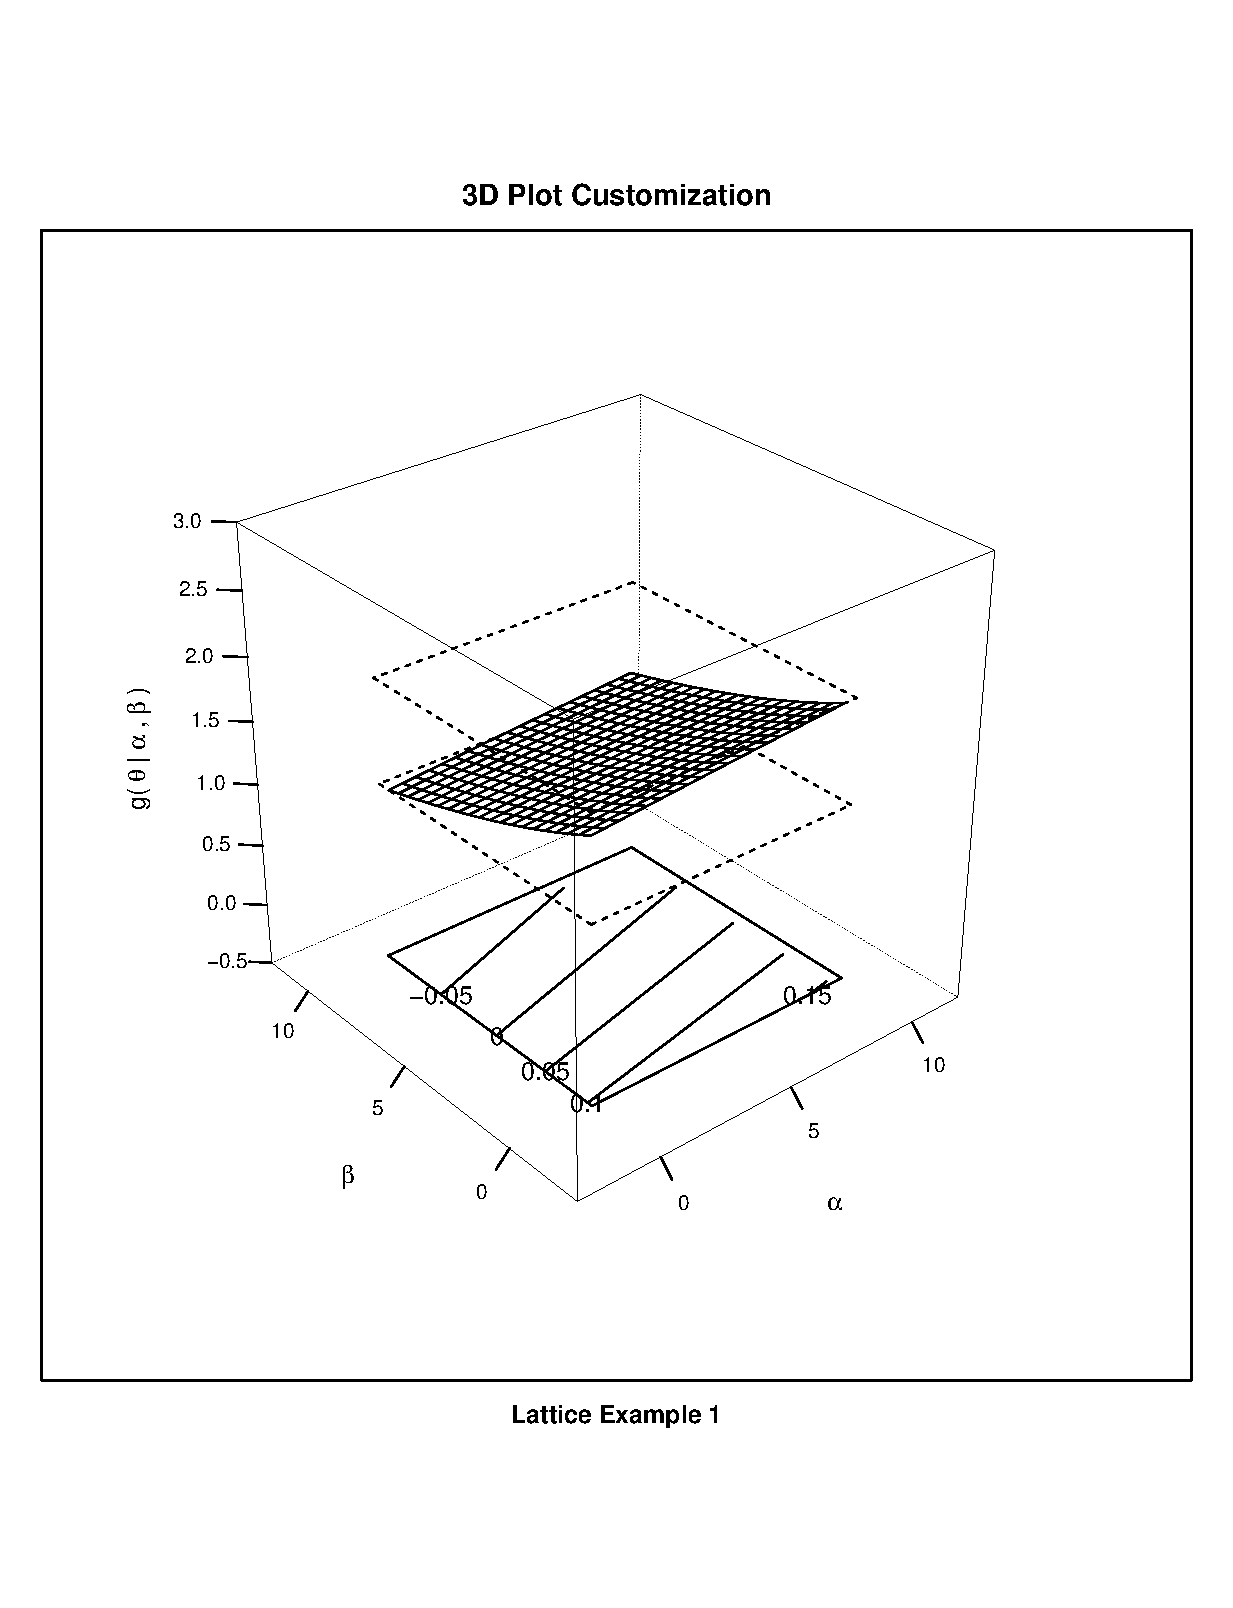
\includegraphics{./img/lattice-fig.eps}


\item \LaTeX 의 문서에 포함될 \texttt{.eps} 그래픽을 \texttt{R}에서 뽑았을 때는 아무런 문제가 없어 보였는데, 정작 \texttt{pdf}로 문서를 뽑아 보니까 이 그래픽이 들어간 페이지가 90도로 돌아가 있거나 혹은 그래픽이 90도로 회전되어 있을 경우에는 아래와 같이 하면 됩니다.

\begin{Schunk}
 \begin{Sinput}
  postscript(file=``filename.eps'', onefile=FALSE, horizontal=FALSE)
 \end{Sinput}
\end{Schunk}

이 문제에 대한 출처는 \texttt{postscript} 도움말입니다.

이문제를 다른 방법으로도 해결할 수 있습니다.  (대충 서너개 더 있음).

\item 새로운 그래픽 객체를 생성하는 방법을 설명해줘서 사용자가 추후에 독립적인 그래픽을 생성할 수 있게 도와주기 


	\item (접수: 2013-APR-23)  저는 다각형을 그리고 싶습니다. 
	
	\textsf{(답변)}  이것은 간단히 2차원-랜덤포인트 생성한 뒤에 \texttt{polygon()} 함수를 써서 보여주면 됨. 

\end{enumerate}

% ggplot2에서 stat_density2d에 오류가 있는것 같습니다. 모든 경우에 NA가 return된다는 보고













\subfile{./Parts/part2.tex}

% %%%%%%%%%%%%%%%%%%%%%%%%%%%%%%%%%%%%%%%%%%%%%%%%%%%%%%%%%%%%%%%%%%%%%%%%%%%%%%%%%%%
%
%
%
%%%%%%%%%%%%%%%%%%%%%%%%%%%%%%%%%%%%%%%%%%%%%%%%%%%%%%%%%%%%%%%%%%%%%%%%%%%%%%%%%%%

\chapter{수학/확률/행렬/수치해석과 관련하여}

\section{수학연산에 도움이 되는 함수들}

\paragraph{행렬값 구하기: }  아마도 행렬과 연관하여 자주 쓰이는 연산은 행렬값을 구하는 것일 것입니다. 
위에서 언급한 M 이라는 행렬값은 $1\times 4 - 3\times 2 = -2$ 일 것입니다. 
R은 이것의 계산을 det()이라는 함수를 이용합니다. 

\begin{Schunk}
\begin{Soutput}
> M <- matrix(c(1,2,3,4), ncol=2)
> val <- det(M)
> M
     [,1] [,2]
[1,]    1    3
[2,]    2    4
> val
[1] -2
> 1*4-3*2
[1] -2
\end{Soutput}
\end{Schunk}


\paragraph{역행렬 찾기:} 역행렬은 \texttt{solve()}라는 함수를 통해 얻을 수 있는데, 수학적인 의미가 $M M^{-1} = I$ 입니다.

\begin{Schunk}
\begin{Soutput}
> solve(M)
     [,1] [,2]
[1,]   -2  1.5
[2,]    1 -0.5
>
\end{Soutput}
\end{Schunk}


\paragraph{연립방정식의 해찾기:} 역행렬을 이용하는 예는 아마도 선형방정식의 해를 구하는 것입니다. 
아래와 같은 선형방정식을 살펴봅니다. 
\begin{eqnarray}
3x + 4y - 2z & = & 5 \\
-4x + 3y - z & = & 22 \\
x + y + z & = & 6
\end{eqnarray}

이는 수학적으로 아래와 같이 쓸 수 있습니다. 

\begin{equation}
	\begin{bmatrix}
		3 & 4 & -2 \\
		-4 & 3 & -1 \\
		1 & 1 & 1 
	\end{bmatrix}
\begin{bmatrix}
	x \\
	y \\
	z 
\end{bmatrix}
= 
\begin{bmatrix}
	5 \\
	-1 \\
	6 
\end{bmatrix}
\end{equation}

이렇게 선형방정식이 $AX=b$라는 형식으로 표현 할 수 있다면 \texttt{solve(M)}의 결과는 \texttt{x}의 해를 의미합니다.
이 선형방정식을 손으로 풀면 $x=1$, $y=2$, $z=3$ 이라는 값이 나오게 됩니다. 
이를 R로 하기위해서는 다음과 같이 할 수 있습니다. 

\begin{Schunk}
\begin{Soutput}
> A <- matrix(c(3,-4,1,4,3,1,-2,-1,1), ncol=3)
> b <- c(5,-1,6)
> solve(A,b)
[1] 1 2 3
> 
\end{Soutput}
\end{Schunk}

\paragraph{텐서 프로닥트}  tensor product (혹은 Kronecker product)란 아래와 같이 행렬의 연산을 수행합니다. 
이를 수행하기 위한 R 함수는 아래와 같습니다. 

\begin{Schunk}
\begin{Soutput}
> A1 <- matrix(c(1,2,3,4), ncol=2)
> A2 <- matrix(1:9, ncol=3)
> kronecker(A1, A2)
     [,1] [,2] [,3] [,4] [,5] [,6]
[1,]    1    4    7    3   12   21
[2,]    2    5    8    6   15   24
[3,]    3    6    9    9   18   27
[4,]    2    8   14    4   16   28
[5,]    4   10   16    8   20   32
[6,]    6   12   18   12   24   36
> 	
\end{Soutput}
\end{Schunk}

\paragraph{외적과 내적}  그런데, 크로넥커 프로닥트는 본래 벡터의 외적을 이용하여 계산합니다. 
외적의 연산에 대한 이해는 아래를 살펴보시길 바랍니다.
\begin{Schunk}
\begin{Soutput}
> x <- 1:9
> names(x) <- x
> x %o% x
  1  2  3  4  5  6  7  8  9
1 1  2  3  4  5  6  7  8  9
2 2  4  6  8 10 12 14 16 18
3 3  6  9 12 15 18 21 24 27
4 4  8 12 16 20 24 28 32 36
5 5 10 15 20 25 30 35 40 45
6 6 12 18 24 30 36 42 48 54
7 7 14 21 28 35 42 49 56 63
8 8 16 24 32 40 48 56 64 72
9 9 18 27 36 45 54 63 72 81
> 
\end{Soutput}
\end{Schunk}

이를 활용하여 구구단을 만드는 프로그램을 작성해봅니다. 

\begin{Schunk}
\begin{Soutput}
> x <- 1:9
> names(x) <- x
> y <- 2:9
> names(y) <- paste(y, "*", sep="")
> outer(y, x, "*")
   1  2  3  4  5  6  7  8  9
2* 2  4  6  8 10 12 14 16 18
3* 3  6  9 12 15 18 21 24 27
4* 4  8 12 16 20 24 28 32 36
5* 5 10 15 20 25 30 35 40 45
6* 6 12 18 24 30 36 42 48 54
7* 7 14 21 28 35 42 49 56 63
8* 8 16 24 32 40 48 56 64 72
9* 9 18 27 36 45 54 63 72 81
> 
\end{Soutput}
\end{Schunk}

\paragraph{고유값과 고유벡터:}  M 행렬의 고유값과 고유벡터는 아래와 같은 방법으로 구할 수 있습니다. 

\begin{Schunk}
\begin{Soutput}
> eM <- eigen(M)
> names(eM)
[1] "values"  "vectors"
> eM$values
[1]  5.3722813 -0.3722813
> eM$vectors
           [,1]       [,2]
[1,] -0.5657675 -0.9093767
[2,] -0.8245648  0.4159736
> 
\end{Soutput}
\end{Schunk}

\paragraph{특이값 분해}

행렬 A의 Singular value decomposition (특이값 분해)는 아래와 같은 수학적 의미를 가집니다. 

\begin{equation}
A = U D(Q) V^T
\end{equation}
%
여기에서 $ U^T U = V^T V = VV^T = I $ 이며 $Q$는 특이값 벡터입니다. 

\begin{Schunk}
\begin{Soutput}
> svdM <- svd(M)
> names(svdM)
[1] "d" "u" "v"
> svdM$d
[1] 5.4649857 0.3659662
> svdM$u
           [,1]       [,2]
[1,] -0.5760484 -0.8174156
[2,] -0.8174156  0.5760484
> svdM$v
           [,1]       [,2]
[1,] -0.4045536  0.9145143
[2,] -0.9145143 -0.4045536
> $
\end{Soutput}
\end{Schunk}


\paragraph{일반 수학함수들}

\paragraph{삼각함수들}
\begin{Schunk}
\begin{Soutput}
output
\end{Soutput}
\end{Schunk}
\paragraph{집합과 관련된 함수들}
\begin{Schunk}
\begin{Soutput}
output
\end{Soutput}
\end{Schunk}
\paragraph{기타 유용한 함수들}
% \item \texttt{which.max()}와 \texttt{which.min()}을 사용하는 방법 
\texttt{combn()} 함수를 이용하여 모든 조합을 찾기

\section{확률의 사용}

\subsection{밀도/누적 확률분포}
\begin{Schunk}
\begin{Soutput}
output
\end{Soutput}
\end{Schunk}

\paragraph{퍼센타일 값 찾기}
\begin{Schunk}
\begin{Soutput}
output
\end{Soutput}
\end{Schunk}

\subsection{표준 난수생성 함수}
\begin{Schunk}
\begin{Soutput}
output
\end{Soutput}
\end{Schunk}

\subsection{비표준 난수생성 알고리즘}
\begin{Schunk}
\begin{Soutput}
output
\end{Soutput}
\end{Schunk}
\paragraph{Multinomial random variables}
\begin{Schunk}
\begin{Soutput}
output
\end{Soutput}
\end{Schunk}

\paragraph{Correlated binary random variables}
\begin{Schunk}
\begin{Soutput}
output
\end{Soutput}
\end{Schunk}

\section{수치해석}
\begin{Schunk}
\begin{Soutput}
output
\end{Soutput}
\end{Schunk}

\subsection{미분}
\begin{Schunk}
\begin{Soutput}
output
\end{Soutput}
\end{Schunk}

\subsection{적분}
\begin{Schunk}
\begin{Soutput}
output
\end{Soutput}
\end{Schunk}
\paragraph{Laplace Approximation} 알고리즘을 구현하는 방법 -- 적분하는 방법에 많이 쓰임 (특히, 베이지안 컴퓨테이션) 
\begin{Schunk}
\begin{Soutput}
output
\end{Soutput}
\end{Schunk}

\subsection{최적화 문제}
\begin{Schunk}
\begin{Soutput}
output
\end{Soutput}
\end{Schunk}
\paragraph{Newton-Raphson} 알고리즘을 구현하는 방법 -- optimization 에 관련된 일종의 설명도 추가해주면 좋을 것 같음 
\begin{Schunk}
\begin{Soutput}
output
\end{Soutput}
\end{Schunk}



\section{시뮬레이션}
\subsection{Metropolis-Hastings} 알고리즘을 구현하는 프레임 워크 - 이것은 그냥 사용가능하게 바로 소스코드 붙여주기 (베이지안 컴퓨테이션에 많이 쓰임)
\begin{Schunk}
\begin{Soutput}
output
\end{Soutput}
\end{Schunk}

\subsection{Bootstrap} 
방법 -- 요건 아주 좋은 패키지가 있음 
\begin{Schunk}
\begin{Soutput}
output
\end{Soutput}
\end{Schunk}


%%%%%%%%%%%%%%%%%%%%%%%%%%%%%%%%%%%%%%%%%%%%%%%%%%%%%%%%%%%%%%%%%%%%%%%%%%%%%%%%%%%
%
%
%
%%%%%%%%%%%%%%%%%%%%%%%%%%%%%%%%%%%%%%%%%%%%%%%%%%%%%%%%%%%%%%%%%%%%%%%%%%%%%%%%%%%

\chapter{탐색적 데이터 분석}

여기에서 말하는 탐색적 분석이란 분석 초기에 단순히 데이터의 특징을 보는데 사용됩니다. 
또한, 이 과정은 데이터 클리닝과도 연관이 있습니다. 

\section{기술통계량 요약}
\begin{Schunk}
\begin{Soutput}
output
\end{Soutput}
\end{Schunk}

\paragraph{평균과 분산과 같은 기초요약 함수들}
\begin{Schunk}
\begin{Soutput}
output
\end{Soutput}
\end{Schunk}

\paragraph{그룹별 평균산출}
\begin{Schunk}
\begin{Soutput}
output
\end{Soutput}
\end{Schunk}

\paragraph{5분위수 구하기}
\begin{Schunk}
\begin{Soutput}
output
\end{Soutput}
\end{Schunk}

\paragraph{퀀타일}
\begin{Schunk}
\begin{Soutput}
output
\end{Soutput}
\end{Schunk}

\paragraph{표준화와 스케일링}
\begin{Schunk}
\begin{Soutput}
output
\end{Soutput}
\end{Schunk}

\paragraph{신뢰구간}
\begin{Schunk}
\begin{Soutput}
output
\end{Soutput}
\end{Schunk}

\section{분할표와 카이제곱 검정}
\begin{Schunk}
\begin{Soutput}
output
\end{Soutput}
\end{Schunk}

\section{z-검정}
\begin{Schunk}
\begin{Soutput}
output
\end{Soutput}
\end{Schunk}

\section{t-검정}
\begin{Schunk}
\begin{Soutput}
output
\end{Soutput}
\end{Schunk}

\section{}
\begin{Schunk}
\begin{Soutput}
output
\end{Soutput}
\end{Schunk}




\chapter{통계모형의 선택 및 적용}

각 섹션은 다음과 같은 방법으로 이루어져야 합니다. 
\begin{itemize}
\item 아래의 모형이 어느 경우에 사용되어야 하는가?
\item 모형을 사용하는데 있어서 요구되는 가정들은 무엇인가?
\item 모형의 계수에 대한 추정치는 어떻게 구하는가?
\item 모형의 진단
\item 추정치들에 대한 해석
\item 사용법들 
\item 모형에 대한 한계점
\end{itemize}

\section{분산분석 (Analysis of Variance-Covariance)}
\begin{Schunk}
\begin{Soutput}
output
\end{Soutput}
\end{Schunk}

\section{상관분석 (Correlation Analysis) }
\begin{Schunk}
\begin{Soutput}
output
\end{Soutput}
\end{Schunk}

\section{회귀분석 (Regression Analysis) }
\begin{Schunk}
\begin{Soutput}
output
\end{Soutput}
\end{Schunk}

\section{주성분분석 (Principle Component Analysis)}
\begin{Schunk}
\begin{Soutput}
output
\end{Soutput}
\end{Schunk}

\section{판별분석 (Discriminant Analysis) }
\begin{Schunk}
\begin{Soutput}
output
\end{Soutput}
\end{Schunk}

\section{군집분석 (Cluster Analysis) }
\begin{Schunk}
\begin{Soutput}
output
\end{Soutput}
\end{Schunk}

\section{시계열분석 (Time-Series Analysis) }
\begin{Schunk}
\begin{Soutput}
output
\end{Soutput}
\end{Schunk}

\section{일반선형모델 (GLM)}
\begin{Schunk}
\begin{Soutput}
output
\end{Soutput}
\end{Schunk}

\section{의사결정 나무(Decision Tree)}
\begin{Schunk}
\begin{Soutput}
output
\end{Soutput}
\end{Schunk}

\section{Longitudinal data analysis}
\begin{Schunk}
\begin{Soutput}
output
\end{Soutput}
\end{Schunk}

\section{생존분석 (Survivial analysis)}
\begin{Schunk}
\begin{Soutput}
output
\end{Soutput}
\end{Schunk}

\section{Mixture and latent class analysis}
\begin{Schunk}
\begin{Soutput}
output
\end{Soutput}
\end{Schunk}

\section{신경망 분석}
\begin{Schunk}
\begin{Soutput}
output
\end{Soutput}
\end{Schunk}

\section{기계학습 (Machine Learning)}
\begin{Schunk}
\begin{Soutput}
output
\end{Soutput}
\end{Schunk}

\section{메타 분석 (Meta Analysis)}
\begin{Schunk}
\begin{Soutput}
output
\end{Soutput}
\end{Schunk}


%%%%%%%%%%%%%%%%%%%%%%%%%%%%%%%%%%%%%%%%%%%%%%%%%%%%%%%%%%%%%%%%%%%%%%%%%%%%%%%%%%%
%
%
%
%%%%%%%%%%%%%%%%%%%%%%%%%%%%%%%%%%%%%%%%%%%%%%%%%%%%%%%%%%%%%%%%%%%%%%%%%%%%%%%%%%%

\section{패키지 관리}
\begin{enumerate}
\item 	이와 반대로 현재 연결된 라이브러리를 떼어낼 수도 있습니다. 

	\begin{Schunk}
	\begin{Soutput}
	> detach(package:pkg_name)	
	\end{Soutput}
	\end{Schunk}

	% 웹에 > detach(package:pkg_name) 과 5. 패키지를 설치 (분류: 사용자 환경)이 한 줄 띄어져야 함.

	\item 패키지를 설치 (분류: 사용자 환경)  
	
	\textsf{(답변)} 설치되는 패키지의 \textbf{설치위치}와 \textbf{의존성}에 대해서 반드시 알아야 합니다. 
	
	\begin{Schunk}
	\begin{Soutput}
	> install.packages("패키지명", dependencies=TRUE, )
	\end{Soutput}
	\end{Schunk}
% 을 쓰지 못하는 사례도 허다하다. package를 설치할 때 메뉴에서 [패키지 -> 패키지 설치하기]를 선택하고 난 뒤
% [mirror]를 선택한 뒤 패키지 리스트에서 하나씩 어디선가 본 패키지 이름을 어렵게 어렵게 찾아 더블클릭하는 절차를 따르는 것이다.

	\item 설치된 패키지의 목록을 확인하는 방법을 알고 싶습니다.
\end{enumerate}


\subfile{./Parts/part3.tex}


% \chapter{Sweave 이해하기}


\chapter{Knitr를 이용한 출력물}


\chapter{\LaTeX Essentials}


\subfile{./Parts/part4.tex}

% %  File tutorial-dev/Parts/part1-ch02.tex
%  Part of the iHELP project at http://ihelp.r-forge.r-project.org
%
%  Copyright (C) 2013- The iHELP Working Group 
%                                in the Korean R Translation Team
%
%  This program is free software; you can redistribute it and/or modify
%  it under the terms of the GNU General Public License as published by
%  the Free Software Foundation; either version 2 of the License, or
%  (at your option) any later version.
%
%  This program is distributed in the hope that it will be useful,
%  but WITHOUT ANY WARRANTY; without even the implied warranty of
%  MERCHANTABILITY or FITNESS FOR A PARTICULAR PURPOSE.  See the
%  GNU General Public License for more details.
%
%  A copy of the GNU General Public License is available at
%  http://www.r-project.org/Licenses/
%


%%%%%%%%%%%%%%%%%%%%%%%%%%%%%%%%%%%%%%%%%%%%%%%%%%%%%%%%%%%%%%%%%%%%%%%%
%
%
%
%
%%%%%%%%%%%%%%%%%%%%%%%%%%%%%%%%%%%%%%%%%%%%%%%%%%%%%%%%%%%%%%%%%%%%%%%%

\documentclass[../tutorial.tex]{subfiles}
\begin{document}


\part{통계모형의 이해와 적용}

\chapter{통계모형의 선택 및 적용}

각 섹션은 다음과 같은 방법으로 이루어져야 합니다. 
\begin{itemize}
\item 아래의 모형이 어느 경우에 사용되어야 하는가?
\item 모형을 사용하는데 있어서 요구되는 가정들은 무엇인가?
\item 모형의 계수에 대한 추정치는 어떻게 구하는가?
\item 모형의 진단
\item 추정치들에 대한 해석
\item 사용법들 
\item 모형에 대한 한계점
\end{itemize}

\section{분산분석 (Analysis of Variance-Covariance)}
\begin{Schunk}
\begin{Soutput}
output
\end{Soutput}
\end{Schunk}

\section{상관분석 (Correlation Analysis) }
\begin{Schunk}
\begin{Soutput}
output
\end{Soutput}
\end{Schunk}

\section{회귀분석 (Regression Analysis) }
\begin{Schunk}
\begin{Soutput}
output
\end{Soutput}
\end{Schunk}

\section{주성분분석 (Principle Component Analysis)}
\begin{Schunk}
\begin{Soutput}
output
\end{Soutput}
\end{Schunk}

\section{판별분석 (Discriminant Analysis) }
\begin{Schunk}
\begin{Soutput}
output
\end{Soutput}
\end{Schunk}

\section{군집분석 (Cluster Analysis) }
\begin{Schunk}
\begin{Soutput}
output
\end{Soutput}
\end{Schunk}

\section{시계열분석 (Time-Series Analysis) }
\begin{Schunk}
\begin{Soutput}
output
\end{Soutput}
\end{Schunk}

\section{일반선형모델 (GLM)}
\begin{Schunk}
\begin{Soutput}
output
\end{Soutput}
\end{Schunk}

\section{의사결정 나무(Decision Tree)}
\begin{Schunk}
\begin{Soutput}
output
\end{Soutput}
\end{Schunk}

\section{Longitudinal data analysis}
\begin{Schunk}
\begin{Soutput}
output
\end{Soutput}
\end{Schunk}

\section{생존분석 (Survivial analysis)}
\begin{Schunk}
\begin{Soutput}
output
\end{Soutput}
\end{Schunk}

\section{Mixture and latent class analysis}
\begin{Schunk}
\begin{Soutput}
output
\end{Soutput}
\end{Schunk}

\section{신경망 분석}
\begin{Schunk}
\begin{Soutput}
output
\end{Soutput}
\end{Schunk}

\section{기계학습 (Machine Learning)}
\begin{Schunk}
\begin{Soutput}
output
\end{Soutput}
\end{Schunk}

\section{메타 분석 (Meta Analysis)}
\begin{Schunk}
\begin{Soutput}
output
\end{Soutput}
\end{Schunk}


%%%%%%%%%%%%%%%%%%%%%%%%%%%%%%%%%%%%%%%%%%%%%%%%%%%%%%%%%%%%%%%%%%%%%%%%%%%%%%%%%%%
%
%
%
%%%%%%%%%%%%%%%%%%%%%%%%%%%%%%%%%%%%%%%%%%%%%%%%%%%%%%%%%%%%%%%%%%%%%%%%%%%%%%%%%%%

\section{패키지 관리}
\begin{enumerate}
\item 	이와 반대로 현재 연결된 라이브러리를 떼어낼 수도 있습니다. 

	\begin{Schunk}
	\begin{Soutput}
	> detach(package:pkg_name)	
	\end{Soutput}
	\end{Schunk}

	% 웹에 > detach(package:pkg_name) 과 5. 패키지를 설치 (분류: 사용자 환경)이 한 줄 띄어져야 함.

	\item 패키지를 설치 (분류: 사용자 환경)  
	
	\textsf{(답변)} 설치되는 패키지의 \textbf{설치위치}와 \textbf{의존성}에 대해서 반드시 알아야 합니다. 
	
	\begin{Schunk}
	\begin{Soutput}
	> install.packages("패키지명", dependencies=TRUE, )
	\end{Soutput}
	\end{Schunk}
% 을 쓰지 못하는 사례도 허다하다. package를 설치할 때 메뉴에서 [패키지 -> 패키지 설치하기]를 선택하고 난 뒤
% [mirror]를 선택한 뒤 패키지 리스트에서 하나씩 어디선가 본 패키지 이름을 어렵게 어렵게 찾아 더블클릭하는 절차를 따르는 것이다.

	\item 설치된 패키지의 목록을 확인하는 방법을 알고 싶습니다.
\end{enumerate}


\end{document}


\subfile{./Parts/part5.tex}

\nocite{GNUR}
\nocite{GNUR-FAQ}

\bibliographystyle{apalike}
\bibliography{tutorial}

\end{document}

% CRAN Repository Policy  -- http://cran.r-project.org/web/packages/policies.html 


% Useful documents
% An Introduction to the interactive debugging tools in R, Roger, D. Peng, UCLA, 
% R Guide: March 2011, L. Chihara 
% Statistical Analysis with R - a quick start - Oleg Nenadic, Walter Zucchini September 2004
% R Package writing tutorial - Harvard Statistics, Alan Lenarcic, August 28, 2007
% Graphical User Interface - http://www.stat.berkely.edu/classes/s244/gui/Gui1.html 
% GUI Development with tcl/tk -- http://wwww.sciviews.org/_rgui/tcltk/Mb.html 
% Interactive 3D plots with the rgl package http://casoilresource.lawr.ucdavis.edu/drupal/node/371 
% Exploring data with statistical graphices in R, Duncan Murdoch, Nov 23 2011, 
% An R-library for 3D visualization with OpenGL, oleg Nenadic, Daniel Adler, Walter Zucchini 
% Advanced Graphics with R, universitat de Barcelona, April 30, 2009. 
% STAT 846 Computational Techniques in Statistics Lecture Notes Longhai 
